\chapter{Guairá}\label{dept:Guaira}
\mapaparaguai{4}{Guairá}
\vfill\clearpage
\clearpage
\subsection*{Análise Temática por Distrito}
\addcontentsline{toc}{subsection}{Análise Temática por Distrito}

Os mapas a seguir mostram, para cada distrito de Guaira, o GSS final (pontuação geral), o risco social (criminalidade e instabilidade) e o potencial de autossuficiência (solo, água e energia). Cada valor é o calculado na metodologia GSS deste guia.

\begin{figure}[htbp]
\centering
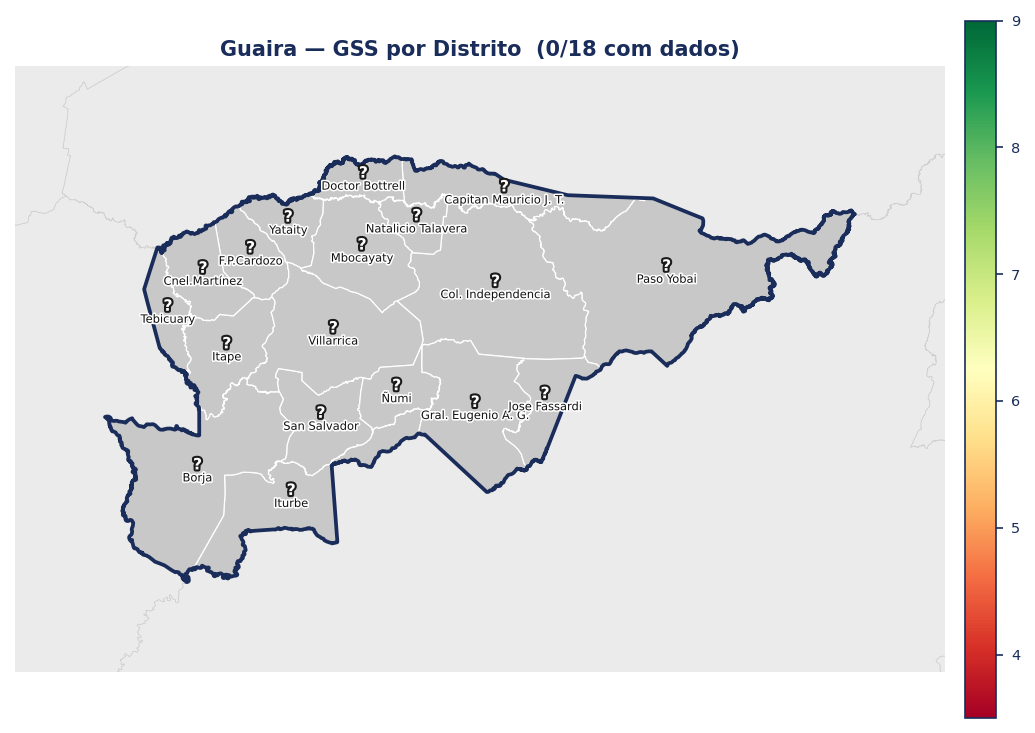
\includegraphics[width=\textwidth, height=0.55\textheight, keepaspectratio]{mapas/mapas_tematicos_dept_04_gss.png}
\caption{GSS (Global Safety Score) por distrito de Guaira. Verde = alta viabilidade · Vermelho = baixa viabilidade.}
\label{fig:gss-04}
\end{figure}

\vspace{0.5em}

\begin{figure}[htbp]
\centering
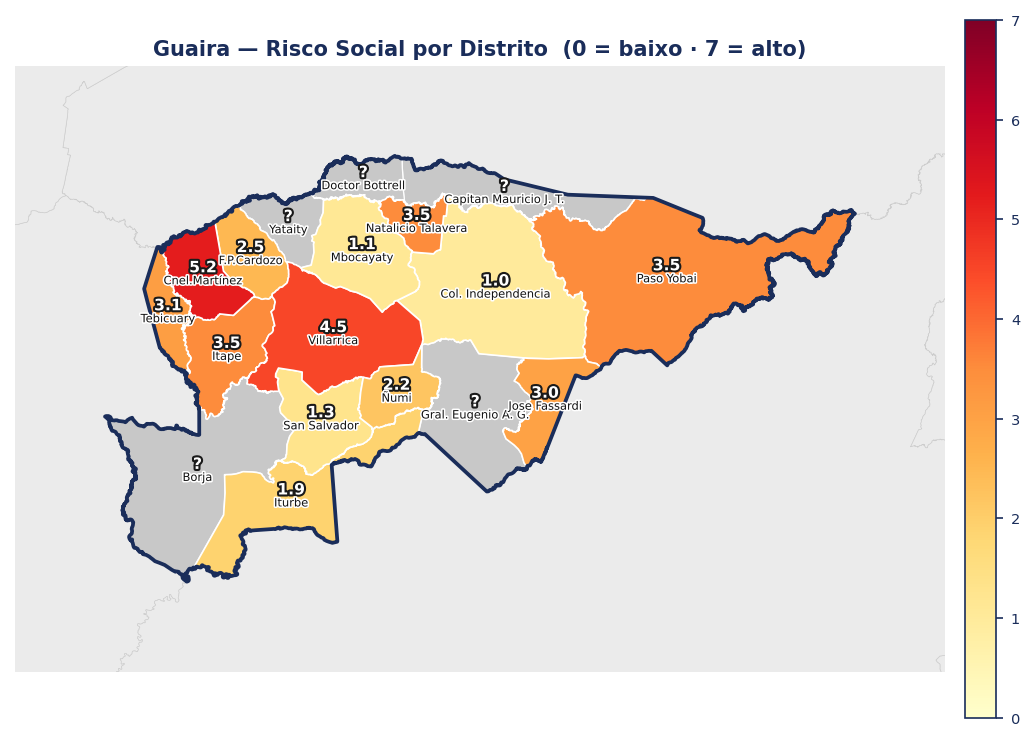
\includegraphics[width=\textwidth, height=0.55\textheight, keepaspectratio]{mapas/mapas_tematicos_dept_04_risco.png}
\caption{Risco social por distrito de Guaira. Amarelo = baixo risco · Vermelho = alto risco.}
\label{fig:risco-04}
\end{figure}

\clearpage

\begin{figure}[htbp]
\centering
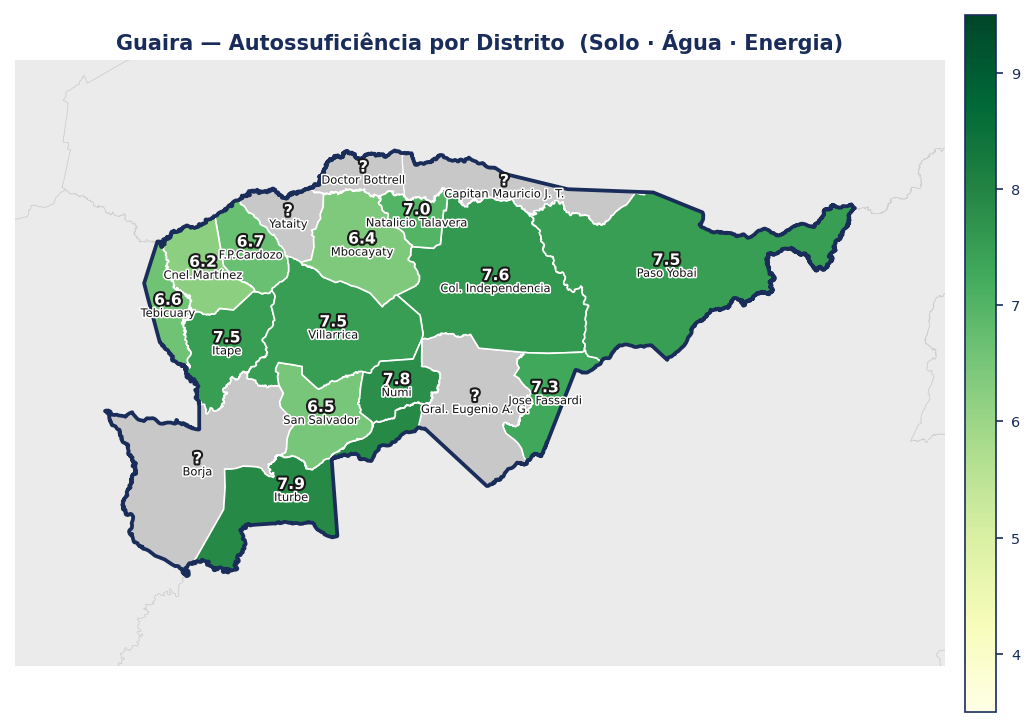
\includegraphics[width=\textwidth, height=0.55\textheight, keepaspectratio]{mapas/mapas_tematicos_dept_04_autosuf.png}
\caption{Autossuficiência por distrito de Guaira: solo, recursos hídricos e potencial energético. Branco = baixo · Verde escuro = alto.}
\label{fig:autosuf-04}
\end{figure}

\clearpage

\section{Guairá}

forte combinacao de turismo, servicos e agricultura.

\subsection{Ficha climática de Villarrica (capital
departamental)}

\textbf{Irradiância solar global --- (kWh/\allowbreak m²/\allowbreak dia):}


\begin{center}
\resizebox{\linewidth}{!}{%
{\renewcommand{\arraystretch}{1.2}%
\begin{tabular}{@{}c|c|c|c|c|c|c|c|c|c|c|c@{}}
\toprule
Jan & Fev & Mar & Abr & Mai & Jun & Jul & Ago & Set & Out & Nov & Dez \\
\midrule
6.74 & 6.20 & 5.50 & 4.48 & 3.35 & 2.88 & 3.21 & 3.96 & 4.59 & 5.43 &
6.43 & 6.81 \\
\bottomrule
\end{tabular}}%
}
\end{center}


Média anual: 4.96 kWh/\allowbreak m²/\allowbreak dia. Inclinação recomendada: 26° Norte (anual);
36° inverno; 16° verão.

\textbf{Precipitação --- (mm/\allowbreak mês):}


\begin{center}
\resizebox{\linewidth}{!}{%
{\renewcommand{\arraystretch}{1.2}%
\begin{tabular}{@{}c|c|c|c|c|c|c|c|c|c|c|c@{}}
\toprule
Jan & Fev & Mar & Abr & Mai & Jun & Jul & Ago & Set & Out & Nov & Dez \\
\midrule
131 & 136 & 131 & 152 & 172 & 90 & 75 & 52 & 92 & 187 & 190 & 166 \\
\bottomrule
\end{tabular}}%
}
\end{center}


Média anual: \textasciitilde1.573 mm/\allowbreak ano. Estação chuvosa Out-Mai; seca
Jun-Set.
\clearpage
\subsection*{Dados Departamentais}

\subsection*{Segurança Pública}

\begin{tabularx}{\linewidth}{lX}
\toprule
Indicador & Valor \\
\midrule
Taxa de homicídios (por 100k hab) & 1,74 (2022, fonte INE/Prosegur) \\
Crimes registrados (total/ano) & --- dados não desagregados publicamente \\
Número de comisarías & ~10 (estimativa departamental) \\
Índice segurança relativo & alto \\
\bottomrule
\end{tabularx}

Guairá apresenta uma das \textbf{menores taxas de homicídios do Paraguai}, com 1,74 por 100 mil habitantes em 2022, colocando-o entre os departamentos mais seguros do país. O Ministerio Público registra que Guairá responde por apenas \textbf{2\% das causas de homicídio doloso} nacional (2019--2024) --- proporção muito baixa e compatível com sua população de cerca de 3\% do total.

O departamento não possui fronteira internacional direta e está localizado na região centro-sul do Paraguai, distante das rotas principais de narcotráfico que afetam os departamentos fronteiriços com Brasil e Argentina. Villarrica, capital do departamento e terceira cidade mais importante do Paraguai, é conhecida por sua estabilidade social e tradição cultural.

A criminalidade é predominantemente patrimonial e de baixa intensidade. Não há registro significativo de atuação de crime organizado transnacional no departamento.

\subsection*{IDH e Desenvolvimento Humano}

\begin{tabularx}{\linewidth}{lX}
\toprule
Indicador & Valor \\
\midrule
IDH & 0,704 \\
Classificação IDH & alto \\
Ranking nacional (1=melhor) & 8/18 \\
Esperança de vida & 72,8 anos \\
Anos de escolaridade média & 8,2 anos \\
RNB per capita (USD PPA) & 8.700 \\
\bottomrule
\end{tabularx}

> Nota: IDH estimado com base no relatório PNUD 2020 e dados subnacionais. Guairá é um departamento de porte médio com economia diversificada (agricultura, indústria têxtil, turismo na Serra do Ybytyruzú). Estimativa baseada em perfil socioeconômico regional.

\begin{tabularx}{\linewidth}{lX}
\toprule
Indicador & Valor \\
\midrule
Taxa de pobreza total (\%) & 34,0\% \\
Taxa de pobreza extrema (\%) & 8,9\% \\
Índice de Gini & 0,455 \\
\bottomrule
\end{tabularx}

> Fonte: INE --- EPHC 2023. Pobreza multidimensional (IPM) de 25,48\% em 2023. Guairá apresenta alta pobreza apesar do IDH razoável, indicando desigualdade interna significativa.

\begin{tabularx}{\linewidth}{lX}
\toprule
Indicador & Valor \\
\midrule
Acesso a água potável (\%) & 76,5\% \\
Acesso a saneamento (\%) & 74,2\% \\
\bottomrule
\end{tabularx}

> Estimativa baseada em dados do Censo 2022. Villarrica, capital departamental, possui boa infraestrutura urbana, mas zonas rurais têm cobertura limitada.

Guairá é um departamento com IDH alto (0,704) e infraestrutura moderada. Villarrica, a capital, é uma cidade histórica e culturalmente vibrante, conhecida como "a Atenas do Paraguai" por sua tradição intelectual. O departamento tem presença de indústrias têxteis, agropecuária e o Parque Nacional Serra de San Rafael. Para brasileiros, destaca-se pela paisagem serrana (Serra do Ybytyruzú), clima agradável e custo de vida moderado. A taxa de pobreza de 34\% é alta e reflete desigualdades internas, mas a capital Villarrica oferece serviços adequados (hospitais regionais, universidades). Acesso a água (76,5\%) e saneamento (74,2\%) são medianos. Oportunidades em agronegócio, turismo ecológico e pequenas indústrias. Comunidade brasileira pequena mas presente.

\subsection*{Sistema Prisional}

{\small
{\small
\begin{tabularx}{\linewidth}{lXXXX}
\toprule
Nome & Município & Capacidade & População & Superlotação \\
\midrule
Penitenciaría Regional de Villarrica & Villarrica & 250 & ~480 & ~192\% \\
\bottomrule
\end{tabularx}
}
}

\begin{tabularx}{\linewidth}{lX}
\toprule
Indicador & Valor \\
\midrule
Total de estabelecimentos & 1 \\
Capacidade total (vagas) & ~250 \\
População carcerária total & ~480 \\
Taxa de superlotação & ~192\% \\
\% presos provisórios & ~66\% \\
\bottomrule
\end{tabularx}

A Penitenciaría Regional de Villarrica é o único estabelecimento penal formal do departamento de Guairá. Villarrica, capital departamental, é uma das cidades históricas do Paraguai e polo educacional e comercial do interior do país.

O presídio sofre de superlotação crônica, com detentos provenientes de todos os 17 municípios do departamento. O perfil de criminalidade local inclui crimes contra a propriedade, tráfico de entorpecentes em escala local e violência doméstica, sendo baixa a presença de crime organizado de grande porte.

O MNP registrou deficiências em assistência médica e jurídica no estabelecimento, com alta proporção de presos em prisão preventiva aguardando julgamento por longos períodos.

\textbf{Para imigrantes:} Guairá é um departamento com boa qualidade de vida relativa, forte tradição agrícola (soja, trigo, pecuária) e clima ameno. O ambiente prisional não representa risco direto para a população geral. A cidade de Villarrica tem infraestrutura urbana razoável e é considerada segura para instalação.

\subsection*{Recursos Hídricos Subterrâneos}

\begin{tabularx}{\linewidth}{lXXX}
\toprule
Aquífero & Cobertura no Dept. & Profundidade Média & Vazão Típica \\
\midrule
Guarani / Misiones (confinado) & ~60\% (porção leste) & 100--350 m & 20--80 m$^3$/h \\
Cristalino (fraturado, Pré-Cambriano) & ~40\% (porção oeste) & 30--100 m & 2--10 m$^3$/h \\
\bottomrule
\end{tabularx}

\begin{tabularx}{\linewidth}{lX}
\toprule
Parâmetro & Valor \\
\midrule
Profundidade média --- Cristalino (m) & 40--100 \\
Profundidade média --- Guarani (m) & 100--350 \\
Profundidade máxima recomendada (m) & 400 \\
Vazão típica (m$^3$/h) & 8--50 \\
Custo estimado perfuração (USD) & 3.000 -- 10.000 \\
Qualidade da água --- Cristalino & boa \\
Qualidade da água --- Guarani & boa a excelente \\
pH médio & 6,5--7,8 \\
Outorga necessária & sim \\
Órgão regulador & MADES --- DGPCRH \\
\bottomrule
\end{tabularx}

Guairá ocupa posição de transição entre o embasamento cristalino e as rochas sedimentares da Bacia do Paraná que hospedam o Aquífero Guarani. O extremo leste do departamento, próximo ao rio Paraná, tem boa cobertura do Guarani com profundidades acessíveis (100--200 m). A cidade de Villarrica (capital) se abastece parcialmente via poços artesianos e rede pública. A qualidade da água subterrânea é geralmente boa, com baixa mineralização. Guairá é reconhecido como área de recarga do Aquífero Guarani. O uso principal é abastecimento doméstico e irrigação agrícola.

Guairá é um departamento com terreno diversificado e produção agrícola expressiva. Para propriedades rurais no leste (Guarani acessível), poço de 100--200 m custa entre USD 3.500 e 8.000 e oferece excelente vazão para irrigação e uso doméstico. Na porção oeste/cristalina, poços de 40--80 m custam menos (USD 2.500--5.000), mas produtividade é mais variável. A rede pública em Villarrica é operada pelo SENASA. Para zonas rurais, poço próprio é a solução padrão.

\subsection*{Aptidão do Solo}

\begin{tabularx}{\linewidth}{lXX}
\toprule
Tipo de Solo & \% do Território & Características \\
\midrule
Ultissolos (Argissolos) & 45\% & Solos podzólicos vermelho-amarelados, textura areno-argilosa, fertilidade média-baixa \\
Oxissolos (Latossolos) & 25\% & Solos derivados de basalto no leste do departamento, maior fertilidade natural \\
Entissolos arenosos & 20\% & Solos arenosos de baixa retenção hídrica e fertilidade; suscetíveis à erosão \\
Aluviais / Inceptissolos & 10\% & Planícies fluviais do Rio Yhú e afluentes; fertilidade moderada \\
\bottomrule
\end{tabularx}

\begin{tabularx}{\linewidth}{lXX}
\toprule
Classe & \% Território & Uso Recomendado \\
\midrule
Lavoura intensiva & 20\% & Soja, milho, trigo (solos basálticos a leste) \\
Lavoura extensiva & 30\% & Mandioca, cana-de-açúcar, algodão, amendoim \\
Pastagem natural & 25\% & Pecuária extensiva \\
Floresta / reserva & 15\% & Matas ciliares, remanescentes de Mata Atlântica Interior \\
Sem aptidão agrícola & 10\% & Áreas urbanas, rochosas e degradadas \\
\bottomrule
\end{tabularx}

\begin{tabularx}{\linewidth}{lX}
\toprule
Parâmetro & Valor \\
\midrule
pH médio & 4,8 -- 5,8 \\
Fertilidade natural & baixa a média \\
Teor de matéria orgânica & baixo (>90\% dos solos cultivados deteriorados) \\
Necessidade de calcário & sim \\
\bottomrule
\end{tabularx}

Guairá tem potencial agrícola moderado, com as melhores áreas localizadas no leste do departamento (solos basálticos mais férteis). Comparativamente, os solos são inferiores aos Latossolos Roxos do Paraná, mas com manejo adequado (calagem, adubação, plantio direto) é possível obter produtividade razoável. O departamento é conhecido por suas cachoeiras (Saltos del Monday) e tem apelo turístico. Para grandes empreendimentos agrícolas mecanizados, Alto Paraná e Itapúa são mais indicados. A terra em Guairá é relativamente acessível para quem busca propriedades menores.

\subsection*{Terra Rural}

\begin{tabularx}{\linewidth}{lXXX}
\toprule
Tipo & Preço (USD/ha) & Faixa & Tendência \\
\midrule
Agrícola alta produtividade & 7.000 & 5.000 -- 10.000 & $\uparrow$ \\
Pastagem & 3.500 & 2.500 -- 5.000 & $\uparrow$ \\
Mata / reserva & 1.500 & 800 -- 2.500 & $\rightarrow$ \\
\bottomrule
\end{tabularx}

\begin{tabularx}{\linewidth}{lX}
\toprule
Parâmetro & Valor \\
\midrule
Valorização anual média (\%) & 7--9\% \\
Lote mínimo rural (ha) & 10 \\
Imposto territorial rural (\%) & 1\% sobre valor fiscal \\
Liquidez do mercado & média--alta \\
\bottomrule
\end{tabularx}

\begin{tabularx}{\linewidth}{lXXX}
\toprule
Indicador & Guairá (PY) & Paraná (BR) & São Paulo interior (BR) \\
\midrule
Terra agrícola (USD/ha) & 5.000--10.000 & 15.000--30.000 & 20.000--45.000 \\
Terra pastagem (USD/ha) & 2.500--5.000 & 6.000--12.000 & 8.000--18.000 \\
Custo relativo & ~35\% do PR & referência PR & referência SP \\
\bottomrule
\end{tabularx}

Guairá é vizinho do Paraná brasileiro e tem características geoclimáticas semelhantes. A diferença de preço de terra chega a 3--5x, sendo muito atrativo para produtores paranaenses que buscam expansão.

\subsection*{Mercado Imobiliário}

\textbf{Capital:} Villarrica

\begin{tabularx}{\linewidth}{lXX}
\toprule
Tipo & Preço (USD/m$^2$) & Aluguel (USD/mês) \\
\midrule
Apartamento 2 quartos & 600 -- 950 & 220 -- 420 \\
Casa 3 quartos & 500 -- 800 & 200 -- 380 \\
\bottomrule
\end{tabularx}

\begin{tabularx}{\linewidth}{lX}
\toprule
Parâmetro & Valor \\
\midrule
Valorização anual (\%) & 5--7\% \\
Disponibilidade de financiamento & boa (cooperativas ativas, BNF) \\
Bairros mais valorizados & Centro histórico, Barrio San Blas, Villa Florida \\
\bottomrule
\end{tabularx}

\textbf{Vale a pena comprar ou alugar?}
Villarrica é uma cidade histórica agradável (aprox. 70.000 hab.) com boa infraestrutura para cidade de interior paraguaio. É conhecida pela produção de artesanato, indústrias têxteis e vitivinicultura na Colônia Independencia (30 km). Para imigrantes com atividade na região, a compra é atrativa dado o baixo custo.

\textbf{Áreas recomendadas:}
O centro de Villarrica e as imediações da Ruta PY08 concentram a melhor oferta imobiliária do departamento, com boa proximidade a serviços, escolas e o comércio local. A Colônia Independencia (30 km) é opção interessante para quem busca ambiente rural com infraestrutura razoável.

\textbf{Armadilhas comuns:}
Parte dos imóveis urbanos mais antigos de Villarrica não possui conexão à rede de esgoto público --- verifique se o imóvel dispõe de fossa asséptica regular ou se há projeto de extensão da rede municipal para o local antes de fechar o negócio.

\subsection*{Cobertura Celular}

{\small
{\small
\begin{tabularx}{\linewidth}{lXXXXX}
\toprule
Operadora & 2G & 3G & 4G & 5G & Cobertura Pop. \\
\midrule
Tigo & 88\% & 78\% & 68\% & --- & 82\% \\
Personal/Claro & 80\% & 70\% & 60\% & --- & 75\% \\
VOX & 50\% & 35\% & 20\% & --- & 42\% \\
\bottomrule
\end{tabularx}
}
}

> \textbf{Nota:} Guairá tem cobertura concentrada em Villarrica (capital, ~120k hab.) e ao longo da Ruta 8 (Coronel Oviedo--Encarnación). Interior serrano e municípios menores têm 3G predominante.

\begin{tabularx}{\linewidth}{lX}
\toprule
Parâmetro & Valor \\
\midrule
Melhor operadora rural & Tigo \\
Velocidade 4G média (Mbps) & 18--35 \\
Áreas sem cobertura & Zonas serranas do leste, áreas de mata \\
Sinal em propriedade rural & moderado \\
\bottomrule
\end{tabularx}

\begin{tabularx}{\linewidth}{lXXX}
\toprule
Plano & Operadora & USD/mês & Dados \\
\midrule
Pré-pago básico (7 dias) & Tigo & ~2,50 & 3 GB \\
Pré-pago intermediário (30 dias) & Personal & ~5,00 & 8 GB \\
Pós-pago entrada & Tigo & ~12,00 & 15 GB + chamadas \\
Pós-pago intermediário & Personal/Claro & ~18,00 & 30 GB + chamadas \\
\bottomrule
\end{tabularx}

\subsection*{Internet}

\begin{tabularx}{\linewidth}{lX}
\toprule
Indicador & Valor \\
\midrule
\% população com internet & ~65\% \\
\% com banda larga fixa & ~22\% dos domicílios \\
Velocidade média download (Mbps) & 25--60 (urbano) / 5--15 (rural) \\
Velocidade média upload (Mbps) & 8--20 (urbano) \\
\bottomrule
\end{tabularx}

\begin{tabularx}{\linewidth}{lXX}
\toprule
Tecnologia & Disponibilidade & Velocidade Típica \\
\midrule
Fibra ótica (FTTH) & Villarrica e municípios principais & 50--300 Mbps \\
Cabo HFC & Villarrica & 30--150 Mbps \\
Rádio/Wireless & Amplo no departamento & 5--50 Mbps \\
ADSL (Copaco) & Interior com rede legada & 2--10 Mbps \\
Satélite (Starlink) & Todo o departamento & 50--200 Mbps \\
\bottomrule
\end{tabularx}

\begin{tabularx}{\linewidth}{lXXX}
\toprule
Provedor & Tecnologia & Área de cobertura & Preço ref. (USD/mês) \\
\midrule
Tigo & Fibra/HFC/Rádio & Villarrica + municípios & 18--50 \\
Claro/Personal & Fibra/Rádio & Villarrica & 15--45 \\
Copaco & ADSL/Rádio & Todo o departamento (rede legada) & 10--28 \\
Starlink & Satélite LEO & Todo o departamento & ~44 + equip. ~370 \\
\bottomrule
\end{tabularx}

A cobertura rural de Guairá é \textbf{moderada}. Villarrica e cidades ao longo da Ruta 8 têm boa conectividade. O interior serrano, especialmente em áreas com topografia acidentada, tem cobertura mais limitada:

\clearpage
\newpage
\secaoDiagnostico{Borja}{\mapaDistrito{0402}}{Borja é um município rural tranquilo no sudoeste do departamento de
Guairá, situado a aproximadamente 30~km de Villarrica pela Ruta~8.
Com cerca de 8.000 habitantes distribuídos em colinas suaves e
campos férteis, combina baixíssima densidade demográfica, forte
tradição de agricultura familiar e clima subtropical ameno. Para o
imigrante brasileiro que prioriza discrição, custo de vida reduzido
e conexão direta com a terra, Borja representa uma escolha sólida
e acessível no coração de Guairá.

\subsubsection{Recomendação Técnica}

Recomendado para perfis agropecuários e famílias que valorizam
sossego rural com razoável acesso à capital departamental. O GSS
de 6.8 reflete segurança institucional elevada, bom ambiente social
e produtividade agrícola consistente, com desconto pela ausência de
banco local e pelo abastecimento de serviços concentrado em
Villarrica. Referência atual de score: GSS 6.8.

}
\begin{table}[ht!]
\small \begin{tabular}{p{3.0cm}p{0.8cm}p{6.0cm}} \toprule
\textbf{Critério} & \textbf{Nota} & \textbf{Justificativa} \\ \midrule
A - Ameaças Estratégicas & 8.0 & Interior distante de fronteiras e eixos de conflito; sem alvos estratégicos relevantes \\
B - Risco Social & 7.0 & Ambiente rural pacífico; criminalidade limitada a abigeato esporádico \\
C - Riscos Naturais & 6.5 & Geologia estável em colinas; risco moderado de alagamentos em baixadas \\
D - Autossuficiência & 5.5 & Boa produção agrícola (soja, milho, pecuária), mas sem banco local e serviços técnicos limitados \\
E - Institucional & 6.5 & Municipalidade funcional; serviços básicos presentes; referência hospitalar em Villarrica \\
\midrule
 \textbf{GSS FINAL} & \textbf{6.8} & \textbf{Seguro (Município rural recomendado para perfis agropecuários que buscam tranquilidade e custo baixo).} \\ \bottomrule
 \end{tabular}
\end{table}
\subsubsection{Vulnerabilidades e
Mitigação}\label{vuln-Borja-vulnerabilidades-e-mitigacao}

\begin{itemize}
\tightlist
\item
  \textbf{Ausência de Banco Local:} Toda movimentação financeira exige
  deslocamento até Villarrica (\textasciitilde 30~km)
  (Mitigação: manter reserva em espécie e usar aplicativos bancários
  digitais via 4G Tigo).
\item
  \textbf{Serviços de Saúde Limitados:} O posto de saúde local cobre
  apenas atenção primária; emergências seguem para Villarrica
  (Mitigação: plano de saúde privado e kit de primeiros socorros
  completo em domicílio).
\item
  \textbf{Risco de Alagamento em Baixadas:} Áreas próximas a arroios
  tributários podem sofrer transbordamentos em períodos de El Niño
  intenso (Mitigação: construção em cotas acima de 160~m e
  mapeamento prévio dos cursos d'água).
\item
  \textbf{Dependência de Serviços em Villarrica:} Comércio especializado,
  ensino médio completo e serviços técnicos concentram-se na capital
  departamental (Mitigação: acesso facilitado pela Ruta~8 asfaltada).
\end{itemize}

\subsubsection{Dossiê de Campo}\label{dossie-Borja-dossie-de-campo}
\begin{description}[style=nextline,leftmargin=0.5cm,font=\bfseries]
\item[Coordenadas]  25°54'S 56°23'W (centro urbano estimado).
\item[Topografia]  Colinas suaves com vales férteis; altitude média \textasciitilde 180~m. Relevo ondulado sem impedimentos à mecanização agrícola. Risco sísmico desprezível.
\item[Alvos Estratégicos]  Nenhum de relevância estratégica elevada; silos de grãos de pequeno porte e frigoríficos locais representam infraestrutura econômica, não alvo militar.
\item[Fallout]  Ventos predominantes de Leste e Sudeste durante a maior parte do ano; Norte-Nordeste no verão. Baixíssimo risco de fallout direto pela distância de qualquer instalação industrial crítica.
\item[População]  \textasciitilde 8.000 habitantes (estimativa Censo 2022). Perfil predominantemente rural (\textgreater 80\%), com forte presença de agricultores familiares.
\item[Densidade]  \textasciitilde 12--16 hab/\allowbreak km² (baixíssima densidade, favorecendo privacidade e isolamento voluntário).
\item[Vias de Acesso]  Acesso principal pela Ruta~8 (Villarrica--Coronel Oviedo), com ramal asfaltado local. Estradas vicinais de terra exigem veículo 4x4 após chuvas intensas.
\item[Serviços]  Posto de saúde (USF); escola primária e ensino médio parcial; feria semanal; sem banco local (caixas eletrônicos em Villarrica). Farmácia local disponível.
\item[Custo de Vida]  Muito baixo; alimentos produzidos localmente; aluguel rural estimado em USD 100--200/\allowbreak mês; terra mais barata que a média departamental.
\item[Preço da Terra]  USD 2.000--5.000/\allowbreak ha (campos de pastagem e lavoura); USD 8.000--12.000/\allowbreak ha (terras mecanizadas em posição privilegiada).
\item[Hidrologia]  Abastecimento pelo Aquífero Guarani (poços artesianos com profundidade 100--250~m). Arroios tributários do Tebicuary-mí em zonas baixas com risco ocasional de alagamento.
\item[Clima]  Subtropical úmido (Cfa/Cwa); temperatura média anual \textasciitilde 22°C; precipitação \textasciitilde 1.580~mm/\allowbreak ano; verões quentes (até 36°C) e invernos amenos com eventuais frentes frias do Sul.
\item[Energia]  Rede da ANDE (Itaipu); cobertura elétrica em área urbana e ao longo das vias principais; zonas rurais distantes podem ter instabilidades. Solar fotovoltaico altamente viável (média 4,9~kWh/m²/dia).
\item[Água]  Excelente via Aquífero Guarani; poços artesianos produtivos com boa qualidade química. Arroios disponíveis para uso agrícola com filtragem.
\item[Qualidade do Solo]  Latossolos vermelhos (Terra Roja) e solos podzólicos nas encostas; pH levemente ácido (5,0--5,5); boa fertilidade natural para soja, milho, mandioca e pastagens.
\item[Recursos Locais]  Soja, milho, pecuária de corte e leiteira; suinocultura; mel; mandioca. Feria semanal com produtos frescos. Potencial para horta familiar e policultura de subsistência.
\item[Segurança]  Zona rural extremamente pacífica. Guairá registra uma das menores taxas de homicídios do Paraguai (\textasciitilde 1,74/\allowbreak 100k hab em 2022). Ocorrências limitam-se a abigeato esporádico.
\item[Leis e Restrições]  Município consolidado no interior do país; sem restrição de fronteira para estrangeiros. Titularidade plena disponível para brasileiros em terras privadas regularizadas.
\end{description}
\textbf{Fonte climática:} NASA POWER Climatology API (período 2001--2020)

\textbf{Fonte luminosa:} estimativa World Atlas of Light Pollution

\paragraph{Irradiação Solar
(kWh/\allowbreak m²/\allowbreak dia)}


\begin{center}
\resizebox{\linewidth}{!}{%
{\renewcommand{\arraystretch}{1.2}%
\begin{tabular}{@{}c|c|c|c|c|c|c|c|c|c|c|c|c@{}}
\toprule
Jan & Fev & Mar & Abr & Mai & Jun & Jul & Ago & Set & Out & Nov & Dez & Média \\
\midrule
6.74 & 6.20 & 5.50 & 4.48 & 3.35 & 2.88 & 3.21 & 3.96 & 4.59 & 5.43 &
6.43 & 6.81 & \textbf{4.96} \\
\bottomrule
\end{tabular}}%
}
\end{center}


\textbf{Inclinação solar recomendada:} 26° N (anual) · 36° N (inverno
jun-ago) · 16° N (verão nov-jan)

\paragraph{Precipitação (mm/\allowbreak mês)}


\begin{center}
\resizebox{\linewidth}{!}{%
{\renewcommand{\arraystretch}{1.2}%
\begin{tabular}{@{}c|c|c|c|c|c|c|c|c|c|c|c|c@{}}
\toprule
Jan & Fev & Mar & Abr & Mai & Jun & Jul & Ago & Set & Out & Nov & Dez & Total/\allowbreak ano \\
\midrule
135 & 130 & 133 & 155 & 168 & 92 & 77 & 60 & 92 & 188 & 189 & 161 &
\textbf{1580 mm} \\
\bottomrule
\end{tabular}}%
}
\end{center}


\paragraph{Poluição Luminosa}

\begin{longtable}[]{@{}ll@{}}
\toprule\noalign{}
Parâmetro & Valor \\
\midrule\noalign{}
\endhead
\bottomrule\noalign{}
\endlastfoot
Escala Bortle & 3--4 --- Céu rural escuro \\
Radiância artificial & \textasciitilde 2,0 nW/\allowbreak cm²/\allowbreak sr \\
\end{longtable}

\paragraph{Solo (SoilGrids 2.0, média ponderada 0--30 cm)}

\begin{longtable}[]{@{}ll@{}}
\toprule\noalign{}
Parâmetro & Valor \\
\midrule\noalign{}
\endhead
\bottomrule\noalign{}
\endlastfoot
pH (H$_2$O) & 5,10 \\
Carbono orgânico (SOC) & 16,2 g/\allowbreak kg \\
Argila & 24,5\% \\
Areia & 49,0\% \\
Silte (calc.) & 26,5\% \\
Densidade aparente & 1,36 g/\allowbreak cm³ \\
\textbf{Aptidão agrícola} & \textbf{Boa (soja, milho, pastagens)} \\
\end{longtable}

\subsubsection{Indicadores Sociais}

\textbf{Fontes:} PNUD 2020, INE\footnote{\fineINE} Censo 2022, INE\footnote{\fineINE} EPHC 2023, Ministerio
Público 2024\\
\textbf{Nota:} Valores marcados como \emph{(dept.)} referem-se ao
departamento de Guairá; valores \emph{(dist.)} são específicos deste
distrito. Dados marcados \emph{(est.)} são estimativas.

\begin{longtable}[]{@{}
  >{\raggedright\arraybackslash}p{(\linewidth - 4\tabcolsep) * \real{0.4231}}
  >{\raggedright\arraybackslash}p{(\linewidth - 4\tabcolsep) * \real{0.2692}}
  >{\raggedright\arraybackslash}p{(\linewidth - 4\tabcolsep) * \real{0.3077}}@{}}
\toprule\noalign{}
\begin{minipage}[b]{\linewidth}\raggedright
Indicador
\end{minipage} & \begin{minipage}[b]{\linewidth}\raggedright
Valor
\end{minipage} & \begin{minipage}[b]{\linewidth}\raggedright
Âmbito
\end{minipage} \\
\midrule\noalign{}
\endhead
\bottomrule\noalign{}
\endlastfoot
IDH (2020) & 0,704 & dept. \\
Ranking IDH nacional & 8/\allowbreak 18 & dept. \\
Esperança de vida & 72,8 anos & dept. \\
Escolaridade média & 7,4 anos & dist. (est.) \\
RNB per capita (USD PPA) & 8.700 & dept. \\
Pobreza monetária (\%) & 34,0\% & dept. \\
Pobreza extrema (\%) & 8,9\% & dept. \\
Índice de Gini & 0,455 & dept. \\
Acesso a água potável (\%) & 76,5\% & dept. \\
Acesso a saneamento (\%) & 74,2\% & dept. \\
Taxa de homicídios (est., /\allowbreak 100k hab) & 1,74 (2022, fonte INE\footnote{\fineINE}/\allowbreak Prosegur) & dept. \\
Índice de segurança & alto & dept. \\
População (Censo 2022) & \textasciitilde 8.000 habitantes & dist. (est.) \\
Idade mediana & N/\allowbreak D & dist. \\
Taxa de fecundidade & N/\allowbreak D & dist. \\
\end{longtable}

\subsubsection{Combustível}

\textbf{Referência:} PETROPAR /\allowbreak  postos locais (2024) \textbf{Tipo de
localidade:} Interior

\begin{longtable}[]{@{}lll@{}}
\toprule\noalign{}
Combustível & USD/\allowbreak litro & Gs/\allowbreak litro (aprox.) \\
\midrule\noalign{}
\endhead
\bottomrule\noalign{}
\endlastfoot
Gasolina 93 oct & 0,97 & 7.178 \\
Gasolina 97 oct (premium) & 1,07 & 7.918 \\
Diesel & 0,90 & 6.660 \\
\end{longtable}

\begin{quote}
Preços podem variar ±5\% conforme posto e sazonalidade. Sem posto
em Borja, recomenda-se abastecer em Villarrica ou ao longo da Ruta~8.
\end{quote}

\subsubsection{Cobertura Celular}

\textbf{Fonte:} CONATEL PY /\allowbreak  operadoras (2024)

\begin{longtable}[]{@{}ll@{}}
\toprule\noalign{}
Parâmetro & Valor \\
\midrule\noalign{}
\endhead
\bottomrule\noalign{}
\endlastfoot
Cobertura 4G população (dept.) & 87\% \\
Cobertura 4G área rural & 70\% \\
Melhor operadora & Tigo \\
Qualidade rural & boa (4G Tigo cobrindo a sede e principais vias) \\
\end{longtable}

\begin{quote}
Para zonas rurais afastadas da sede municipal, recomenda-se chip Tigo
como principal e Personal como backup. Starlink disponível como
alternativa de alta velocidade.
\end{quote}

\subsubsection{Internet}

\textbf{Fonte:} CONATEL /\allowbreak  Speedtest Ookla (2024)

\begin{longtable}[]{@{}ll@{}}
\toprule\noalign{}
Parâmetro & Valor \\
\midrule\noalign{}
\endhead
\bottomrule\noalign{}
\endlastfoot
Velocidade média download & 40--50 Mbps (área urbana) \\
Domicílios com internet (dept.) & 60\% \\
Tecnologia predominante & rádio / 4G fixo \\
Opção rural & Starlink disponível (\textasciitilde USD 44/\allowbreak mês) \\
\end{longtable}

\subsubsection{Mercado Imobiliário e Terra Rural}

\textbf{Fonte:} INDERT /\allowbreak  Clasificados.com.py (2024)

\begin{longtable}[]{@{}ll@{}}
\toprule\noalign{}
Tipo & Referência \\
\midrule\noalign{}
\endhead
\bottomrule\noalign{}
\endlastfoot
Terra agrícola (soja/milho) (USD/\allowbreak ha) & 3.500--5.500 \\
Terra de pastagem (USD/\allowbreak ha) & 2.000--3.500 \\
Imóvel urbano (USD/\allowbreak m²) & 300--500 \\
Aluguel casa rural (USD/\allowbreak mês) & 100--200 \\
\end{longtable}

\begin{quote}
Valores sensivelmente abaixo da média departamental por ser município
pequeno sem polo industrial. Boa relação custo-benefício para
estabelecimentos rurais de médio porte.
\end{quote}

\subsubsection{Saúde}

\textbf{Fonte:} MSPBS /\allowbreak  IPS Paraguay (2024--2026), consolidação
departamental e proxy local

\begin{longtable}[]{@{}ll@{}}
\toprule\noalign{}
Serviço & Disponibilidade \\
\midrule\noalign{}
\endhead
\bottomrule\noalign{}
\endlastfoot
USF /\allowbreak  Posto de Saúde & sim \\
Hospital Regional & não (referência em Villarrica) \\
IPS (seguro social) & não \\
Farmácia & sim (farmácia local) \\
Distância ao hospital de referência & \textasciitilde 30~km (Villarrica) \\
\end{longtable}

\textbf{Principais estabelecimentos:} USF local para atenção primária;
Hospital Regional de Villarrica como referência para média e alta
complexidade.

\textbf{Observação para imigrantes:} Atenção primária disponível
localmente; casos de maior complexidade requerem deslocamento a
Villarrica (\textasciitilde 30~min pela Ruta~8). Cobertura privada fortemente
recomendada para especialidades e emergências cirúrgicas.
\newpage
\secaoDiagnostico{Capitan Mauricio Jose Troche}{\mapaDistrito{0403}}{Capitán Mauricio José Troche é um município rural tranquilo no nordeste
do departamento de Guairá, próximo à Serra de San Joaquín. Com cerca de
9.000 habitantes distribuídos em colinas com mata ciliar, combina
economia agropecuária sólida (soja, milho, pecuária) com baixíssima
densidade demográfica e acesso ao Aquífero Guarani. Situado a
\textasciitilde 180~km de Assunção pela Ruta~8, o município homenageia
o herói da Guerra da Tríplice Aliança Capitán Mauricio José Troche.
Para o imigrante que prioriza discrição, custo de vida baixo e
conexão com a terra, Troche representa uma escolha sólida no interior
de Guairá.

\subsubsection{Recomendação Técnica}

Recomendado para perfis agropecuários e famílias que valorizam sossego
rural com acesso razoável à capital departamental. O GSS de 7.3 reflete
segurança institucional elevada, bom ambiente social e produtividade
agrícola consistente em região de colinas com boa disponibilidade
hídrica. Referência atual de score: GSS 7.3.

}
\begin{table}[ht!]
\small \begin{tabular}{p{3.0cm}p{0.8cm}p{6.0cm}} \toprule
\textbf{Critério} & \textbf{Nota} & \textbf{Justificativa} \\ \midrule
A - Ameaças Estratégicas & 8.0 & Interior distante de fronteiras e eixos de conflito; sem alvos estratégicos relevantes \\
B - Risco Social & 7.5 & Ambiente rural pacífico; criminalidade muito baixa; forte coesão comunitária agropecuária \\
C - Riscos Naturais & 7.0 & Colinas com geologia estável; risco moderado de alagamentos pontuais em baixadas \\
D - Autossuficiência & 6.5 & Boa produção agropecuária (soja, milho, pecuária), mas serviços especializados em Villarrica \\
E - Institucional & 7.0 & Municipalidade funcional; serviços básicos presentes; referência hospitalar em Villarrica \\
\midrule
 \textbf{GSS FINAL} & \textbf{7.3} & \textbf{Seguro (Município rural recomendado para perfis agropecuários que buscam tranquilidade e custo baixo).} \\ \bottomrule
 \end{tabular}
\end{table}
\subsubsection{Vulnerabilidades e Mitigação}\label{vuln-Capitan_Mauricio_Jose_Troche-vulnerabilidades-e-mitigacao}

\begin{itemize}
\tightlist
\item
  \textbf{Ausência de Banco Local:} Movimentação financeira exige
  deslocamento até Villarrica ou Coronel Oviedo
  (Mitigação: manter reserva em espécie e usar aplicativos bancários
  digitais via 4G Tigo).
\item
  \textbf{Serviços de Saúde Limitados:} O posto de saúde local cobre
  apenas atenção primária; emergências seguem para Villarrica
  (Mitigação: plano de saúde privado e kit de primeiros socorros
  completo em domicílio).
\item
  \textbf{Risco de Alagamento em Baixadas:} Áreas próximas a arroios
  tributários podem sofrer transbordamentos em períodos de El Niño
  intenso (Mitigação: construção em cotas elevadas nas colinas e
  mapeamento prévio dos cursos d'água).
\item
  \textbf{Cobertura Celular Moderada:} 4G disponível na sede, mas com
  cobertura irregular em zonas rurais afastadas
  (Mitigação: chip Tigo como principal e Starlink como backup em
  propriedades rurais remotas).
\end{itemize}

\subsubsection{Dossiê de Campo}\label{dossie-Capitan_Mauricio_Jose_Troche-dossie-de-campo}
\begin{description}[style=nextline,leftmargin=0.5cm,font=\bfseries]
\item[Coordenadas]  25°29'S 56°07'W (centro urbano estimado).
\item[Topografia]  Região de colinas com mata ciliar; altitude média \textasciitilde 200--250~m. Relevo ondulado próximo à Serra de San Joaquín. Risco sísmico desprezível.
\item[Alvos Estratégicos]  Nenhum de relevância estratégica elevada; silos de grãos de pequeno porte representam infraestrutura econômica local, não alvo militar.
\item[Fallout]  Ventos predominantes de Leste e Sudeste durante a maior parte do ano; Norte-Nordeste no verão. Baixíssimo risco de fallout direto pela distância de qualquer instalação industrial crítica.
\item[População]  \textasciitilde 9.000 habitantes (estimativa Censo 2022). Perfil predominantemente rural (\textgreater 80\%), com forte presença de agricultores e pecuaristas.
\item[Densidade]  \textasciitilde 15--20 hab/\allowbreak km² (baixa densidade, favorecendo privacidade e isolamento voluntário).
\item[Vias de Acesso]  Acesso pela Ruta~8 (Villarrica--Coronel Oviedo) com ramal local; \textasciitilde 180~km de Assunção. Estradas vicinais de terra exigem veículo 4x4 após chuvas intensas.
\item[Serviços]  Posto de saúde (USF); escola primária e ensino médio parcial; feria semanal; sem banco local (caixas eletrônicos em Villarrica ou Coronel Oviedo). Farmácia local disponível.
\item[Custo de Vida]  Muito baixo; alimentos produzidos localmente; aluguel rural estimado em USD 100--200/\allowbreak mês; terra abaixo da média departamental.
\item[Preço da Terra]  USD 2.500--5.500/\allowbreak ha (campos de pastagem e lavoura); USD 6.000--9.000/\allowbreak ha (terras mecanizadas em posição privilegiada).
\item[Hidrologia]  Abastecimento pelo Aquífero Guarani (poços artesianos com profundidade 100--250~m). Arroios tributários em zonas baixas com risco ocasional de alagamento.
\item[Clima]  Subtropical úmido (Cfa/Cwa); temperatura média anual \textasciitilde 22°C; precipitação \textasciitilde 1.580~mm/\allowbreak ano; verões quentes (até 36°C) e invernos amenos com eventuais frentes frias do Sul.
\item[Energia]  Rede da ANDE (Itaipu); cobertura elétrica na área urbana e ao longo das vias principais; zonas rurais distantes podem ter instabilidades. Solar fotovoltaico altamente viável (média \textasciitilde 4,9~kWh/m²/dia).
\item[Água]  Excelente via Aquífero Guarani; poços artesianos produtivos com boa qualidade química. Arroios disponíveis para uso agrícola com filtragem.
\item[Qualidade do Solo]  Latossolos vermelhos (Terra Roja) e solos podzólicos nas encostas; pH levemente ácido (5,0--5,5); boa fertilidade natural para soja, milho, mandioca e pastagens.
\item[Recursos Locais]  Soja, milho, pecuária de corte e leiteira; mandioca; mel. Feria semanal com produtos frescos. Potencial para horta familiar e policultura de subsistência.
\item[Segurança]  Zona rural extremamente pacífica. Guairá registra uma das menores taxas de homicídios do Paraguai (\textasciitilde 1,74/\allowbreak 100k hab em 2022). Ocorrências limitam-se a abigeato esporádico.
\item[Leis e Restrições]  Município consolidado no interior do país; sem restrição de fronteira para estrangeiros. Titularidade plena disponível para brasileiros em terras privadas regularizadas.
\end{description}
\textbf{Fonte climática:} NASA POWER Climatology API (período 2001--2020)

\textbf{Fonte luminosa:} estimativa World Atlas of Light Pollution

\paragraph{Irradiação Solar
(kWh/\allowbreak m²/\allowbreak dia)}


\begin{center}
\resizebox{\linewidth}{!}{%
{\renewcommand{\arraystretch}{1.2}%
\begin{tabular}{@{}c|c|c|c|c|c|c|c|c|c|c|c|c@{}}
\toprule
Jan & Fev & Mar & Abr & Mai & Jun & Jul & Ago & Set & Out & Nov & Dez & Média \\
\midrule
6.74 & 6.20 & 5.50 & 4.48 & 3.35 & 2.88 & 3.21 & 3.96 & 4.59 & 5.43 &
6.43 & 6.81 & \textbf{4.96} \\
\bottomrule
\end{tabular}}%
}
\end{center}


\textbf{Inclinação solar recomendada:} 26° N (anual) · 36° N (inverno
jun-ago) · 16° N (verão nov-jan)

\paragraph{Precipitação (mm/\allowbreak mês)}


\begin{center}
\resizebox{\linewidth}{!}{%
{\renewcommand{\arraystretch}{1.2}%
\begin{tabular}{@{}c|c|c|c|c|c|c|c|c|c|c|c|c@{}}
\toprule
Jan & Fev & Mar & Abr & Mai & Jun & Jul & Ago & Set & Out & Nov & Dez & Total/\allowbreak ano \\
\midrule
135 & 130 & 133 & 155 & 168 & 92 & 77 & 60 & 92 & 188 & 189 & 161 &
\textbf{1580 mm} \\
\bottomrule
\end{tabular}}%
}
\end{center}


\paragraph{Poluição Luminosa}

\begin{longtable}[]{@{}ll@{}}
\toprule\noalign{}
Parâmetro & Valor \\
\midrule\noalign{}
\endhead
\bottomrule\noalign{}
\endlastfoot
Escala Bortle & 3--4 --- Céu rural escuro \\
Radiância artificial & \textasciitilde 2,0 nW/\allowbreak cm²/\allowbreak sr \\
\end{longtable}

\paragraph{Solo (SoilGrids 2.0, média ponderada 0--30 cm)}

\begin{longtable}[]{@{}ll@{}}
\toprule\noalign{}
Parâmetro & Valor \\
\midrule\noalign{}
\endhead
\bottomrule\noalign{}
\endlastfoot
pH (H$_2$O) & 5,10 \\
Carbono orgânico (SOC) & 16,5 g/\allowbreak kg \\
Argila & 25,0\% \\
Areia & 49,5\% \\
Silte (calc.) & 25,5\% \\
Densidade aparente & 1,34 g/\allowbreak cm³ \\
\textbf{Aptidão agrícola} & \textbf{Boa (soja, milho, pastagens)} \\
\end{longtable}

\subsubsection{Indicadores Sociais}

\textbf{Fontes:} PNUD 2020, INE\footnote{\fineINE} Censo 2022, INE\footnote{\fineINE} EPHC 2023, Ministerio
Público 2024\\
\textbf{Nota:} Valores marcados como \emph{(dept.)} referem-se ao
departamento de Guairá; valores \emph{(dist.)} são específicos deste
distrito. Dados marcados \emph{(est.)} são estimativas.

\begin{longtable}[]{@{}
  >{\raggedright\arraybackslash}p{(\linewidth - 4\tabcolsep) * \real{0.4231}}
  >{\raggedright\arraybackslash}p{(\linewidth - 4\tabcolsep) * \real{0.2692}}
  >{\raggedright\arraybackslash}p{(\linewidth - 4\tabcolsep) * \real{0.3077}}@{}}
\toprule\noalign{}
\begin{minipage}[b]{\linewidth}\raggedright
Indicador
\end{minipage} & \begin{minipage}[b]{\linewidth}\raggedright
Valor
\end{minipage} & \begin{minipage}[b]{\linewidth}\raggedright
Âmbito
\end{minipage} \\
\midrule\noalign{}
\endhead
\bottomrule\noalign{}
\endlastfoot
IDH (2020) & 0,704 & dept. \\
Ranking IDH nacional & 8/\allowbreak 18 & dept. \\
Esperança de vida & 72,8 anos & dept. \\
Escolaridade média & 7,4 anos & dist. (est.) \\
RNB per capita (USD PPA) & 8.700 & dept. \\
Pobreza monetária (\%) & 34,0\% & dept. \\
Pobreza extrema (\%) & 8,9\% & dept. \\
Índice de Gini & 0,455 & dept. \\
Acesso a água potável (\%) & 76,5\% & dept. \\
Acesso a saneamento (\%) & 74,2\% & dept. \\
Taxa de homicídios (est., /\allowbreak 100k hab) & 1,74 (2022, fonte INE\footnote{\fineINE}/\allowbreak Prosegur) & dept. \\
Índice de segurança & alto & dept. \\
População (Censo 2022) & \textasciitilde 9.000 habitantes & dist. (est.) \\
Idade mediana & N/\allowbreak D & dist. \\
Taxa de fecundidade & N/\allowbreak D & dist. \\
\end{longtable}

\subsubsection{Combustível}

\textbf{Referência:} PETROPAR /\allowbreak  postos locais (2024) \textbf{Tipo de
localidade:} Interior

\begin{longtable}[]{@{}lll@{}}
\toprule\noalign{}
Combustível & USD/\allowbreak litro & Gs/\allowbreak litro (aprox.) \\
\midrule\noalign{}
\endhead
\bottomrule\noalign{}
\endlastfoot
Gasolina 93 oct & 0,97 & 7.178 \\
Gasolina 97 oct (premium) & 1,07 & 7.918 \\
Diesel & 0,90 & 6.660 \\
\end{longtable}

\begin{quote}
Preços podem variar ±5\% conforme posto e sazonalidade. Sem posto
local, recomenda-se abastecer em Villarrica ou ao longo da Ruta~8.
\end{quote}

\subsubsection{Cobertura Celular}

\textbf{Fonte:} CONATEL PY /\allowbreak  operadoras (2024)

\begin{longtable}[]{@{}ll@{}}
\toprule\noalign{}
Parâmetro & Valor \\
\midrule\noalign{}
\endhead
\bottomrule\noalign{}
\endlastfoot
Cobertura 4G população (dept.) & 87\% \\
Cobertura 4G área rural & 60--70\% \\
Melhor operadora & Tigo \\
Qualidade rural & moderada (4G Tigo cobrindo sede e principais vias) \\
\end{longtable}

\begin{quote}
Para zonas rurais afastadas da sede municipal, recomenda-se chip Tigo
como principal e Personal como backup. Starlink disponível como
alternativa de alta velocidade em propriedades remotas.
\end{quote}

\subsubsection{Internet}

\textbf{Fonte:} CONATEL /\allowbreak  Speedtest Ookla (2024)

\begin{longtable}[]{@{}ll@{}}
\toprule\noalign{}
Parâmetro & Valor \\
\midrule\noalign{}
\endhead
\bottomrule\noalign{}
\endlastfoot
Velocidade média download & 30--45 Mbps (área urbana) \\
Domicílios com internet (dept.) & 60\% \\
Tecnologia predominante & rádio / 4G fixo \\
Opção rural & Starlink disponível (\textasciitilde USD 44/\allowbreak mês) \\
\end{longtable}

\subsubsection{Mercado Imobiliário e Terra Rural}

\textbf{Fonte:} INDERT /\allowbreak  Clasificados.com.py (2024)

\begin{longtable}[]{@{}ll@{}}
\toprule\noalign{}
Tipo & Referência \\
\midrule\noalign{}
\endhead
\bottomrule\noalign{}
\endlastfoot
Terra agrícola (soja/milho) (USD/\allowbreak ha) & 3.000--5.500 \\
Terra de pastagem (USD/\allowbreak ha) & 2.000--3.500 \\
Imóvel urbano (USD/\allowbreak m²) & 300--500 \\
Aluguel casa rural (USD/\allowbreak mês) & 100--200 \\
\end{longtable}

\begin{quote}
Valores sensivelmente abaixo da média departamental por ser município
pequeno sem polo industrial. Boa relação custo-benefício para
estabelecimentos rurais de médio porte.
\end{quote}

\subsubsection{Saúde}

\textbf{Fonte:} MSPBS /\allowbreak  IPS Paraguay (2024--2026), consolidação
departamental e proxy local

\begin{longtable}[]{@{}ll@{}}
\toprule\noalign{}
Serviço & Disponibilidade \\
\midrule\noalign{}
\endhead
\bottomrule\noalign{}
\endlastfoot
USF /\allowbreak  Posto de Saúde & sim \\
Hospital Regional & não (referência em Villarrica) \\
IPS (seguro social) & não \\
Farmácia & sim (farmácia local) \\
Distância ao hospital de referência & \textasciitilde 40--50~km (Villarrica) \\
\end{longtable}

\textbf{Principais estabelecimentos:} USF local para atenção primária;
Hospital Regional de Villarrica como referência para média e alta
complexidade.

\textbf{Observação para imigrantes:} Atenção primária disponível
localmente; casos de maior complexidade requerem deslocamento a
Villarrica. Cobertura privada fortemente recomendada para especialidades
e emergências cirúrgicas.
\newpage
\secaoDiagnostico{Coronel Martinez}{\mapaDistrito{0404}}{Coronel Martínez é uma localidade marcada pela monocultura da
cana-de-açúcar e pela extrema vulnerabilidade hidrológica. Embora esteja
situada em um departamento seguro e tenha solos férteis, o risco de
isolamento físico durante as cheias do Rio Tebicuary-mí penaliza
severamente seu score GSS. É um local que exige alta preparação em
termos de logística de emergência e autonomia de suprimentos.

\subsubsection{Recomendação
Técnica}

Indicado apenas para quem possa investir em terrenos em cotas elevadas e
possua meios de transporte redundantes (inclusive aquáticos). Não
recomendado para residência principal de perfis que necessitem de acesso
diário a serviços urbanos sem interrupções. Referência atual de score:
GSS 5.2.

}
\begin{table}[ht!]
\small \begin{tabular}{p{3.0cm}p{0.8cm}p{6.0cm}} \toprule
\textbf{Critério} & \textbf{Nota} & \textbf{Justificativa} \\ \midrule
A - Ameaças Estratégicas & 5.8 & Proximidade com usina industrial estratégica; visibilidade logística secundária \\
B - Risco Social & 4.8 & Densidade moderada, mas penalizada pela vulnerabilidade extrema de acesso \\
C - Riscos Naturais & 3.5 & Geologia estável; nota baixa devido ao risco crítico de inundação e isolamento hídrico \\
D - Autossuficiência & 6.2 & Recursos agrícolas focados em cana; água abundante mas com risco de contaminação superficial \\
E - Institucional & 5.3 & Ambiente institucional funcional, mas dependente de recursos externos para gestão de desastres \\
\midrule
 \textbf{GSS FINAL} & \textbf{5.2} & \textbf{Sensivel (Localidade que exige mitigação hidrológica robusta e autonomia logística).} \\ \bottomrule
 \end{tabular}
\end{table}
\subsubsection{Vulnerabilidades e
Mitigação}\label{vuln-Coronel_Martinez-vulnerabilidades-e-mitigauxe7uxe3o}

\begin{itemize}
\tightlist
\item
  \textbf{Risco Hídrico Extremo:} Isolamento físico por cheias do Rio
  Tebicuary-mí (Mitigação: construção em cotas \textgreater150m, posse
  de embarcações leves e rádio-comunicação).
\item
  \textbf{Dependência Industrial:} Economia atrelada à usina AZPA
  (Mitigação: diversificação para agricultura de subsistência e pequenos
  animais).
\item
  \textbf{Logística Crítica:} Dependência de poucas pontes e rotas
  asfálticas que podem ser bloqueadas por inundações (Mitigação:
  mapeamento de rotas de fuga por terraplenagem em direção a
  Villarrica).
\end{itemize}

\subsubsection{Dossiê de Campo}\label{dossie-Coronel_Martinez-dossiuxea-de-campo}
\begin{description}[style=nextline,leftmargin=0.5cm,font=\bfseries]
\item[Coordenadas]  25°45'S 56°37'W.
\item[Topografia]  Relevo predominantemente plano com áreas de várzea e "esteros" (áreas úmidas). Altitude \textasciitilde 130m. Geologicamente estável.
\item[Alvos Estratégicos]  Proximidade com a Usina AZPA (Azucarera Paraguaya S.A.) em Tebicuary (1,9 km); Eixo de transporte de cana-de-açúcar; Estação ferroviária histórica.
\item[Fallout]  Ventos predominantes de Sudeste (SE) e Sul-Sudeste (SSE). Baixo risco de fallout direto.
\item[População]  4.505 habitantes (Censo 2022 Final). Perfil equilibrado entre zona urbana (51\%) e rural (49\%).
\item[Densidade]  \textasciitilde 26,6 hab/\allowbreak km² (Baixa densidade, mas com núcleos rurais vulneráveis ao isolamento físico).
\item[Vias de Acesso]  Acesso asfáltico conectando a Villarrica (22 km) e à Ruta PY08. Contudo, vias secundárias e acessos a companhias rurais são críticos e frequentemente interrompidos por cheias.
\item[Serviços]  Unidade de Saúde da Família (USF) local para atendimentos primários. Dependência total do Hospital Regional de Villarrica para alta complexidade.
\item[Custo de Vida]  Muito baixo; economia baseada quase exclusivamente na cana-de-açúcar.
\item[Preço da Terra]  US\$ 5.000-10.000/\allowbreak ha (terras mecanizáveis para cana); valores elevados pela proximidade com a indústria açucareira de Tebicuary.
\item[Hidrologia]  Risco Crítico de Inundação e Isolamento. O Rio Tebicuary-mí transborda com frequência. A localidade de Capellán Egidio Cardozo sofre isolamento periódico, exigindo transporte por canoas ou tratores em eventos de chuva extrema (>500mm acumulados).
\item[Clima]  Tropical Úmido. Verões com temperaturas extremas e alta pluviosidade (1.600 mm/\allowbreak ano).
\item[Energia]  Rede nacional (Itaipu); interrupções frequentes em áreas rurais durante tempestades.
\item[Água]  Poços artesianos e lençol freático superficial (vulnerável a contaminação em áreas de estero).
\item[Qualidade do Solo]  Alfisois e Ultisois (argilosos e ricos em ferro); alta fertilidade para cana-de-açúcar, mas drenagem deficiente em áreas baixas.
\item[Recursos Locais]  Grande produção de cana-de-açúcar e gado de subsistência. Potencial de autossuficiência limitado pela monocultura industrial da região.
\item[Segurança]  Zona rural pacata. Guairá é um dos departamentos mais seguros do Paraguai (\textasciitilde 6,0/\allowbreak 100k homicídios). Conflitos sociais ocasionais ligados a preços de cana-de-açúcar e logística industrial.
\item[Leis Local: Município consolidado. Livre de Restrição de Fronteira]  Localizado no interior, sem impedimentos para brasileiros em terras privadas tituladas.
\end{description}
\textbf{Fonte climática:} NASA POWER Climatology API (período 2001-2020)

\textbf{Fonte luminosa:} estimativa world atlas

\paragraph{Irradiação Solar
(kWh/\allowbreak m²/\allowbreak dia)}


\begin{center}
\resizebox{\linewidth}{!}{%
{\renewcommand{\arraystretch}{1.2}%
\begin{tabular}{@{}c|c|c|c|c|c|c|c|c|c|c|c|c@{}}
\toprule
Jan & Fev & Mar & Abr & Mai & Jun & Jul & Ago & Set & Out & Nov & Dez & Média \\
\midrule
6.74 & 6.20 & 5.50 & 4.48 & 3.35 & 2.88 & 3.21 & 3.96 & 4.59 & 5.43 &
6.43 & 6.81 & \textbf{4.96} \\
\bottomrule
\end{tabular}}%
}
\end{center}


\textbf{Inclinação solar recomendada:} 26° N (anual) · 36° N (inverno
jun-ago) · 16° N (verão nov-jan)

\paragraph{Precipitação (mm/\allowbreak mês)}


\begin{center}
\resizebox{\linewidth}{!}{%
{\renewcommand{\arraystretch}{1.2}%
\begin{tabular}{@{}c|c|c|c|c|c|c|c|c|c|c|c|c@{}}
\toprule
Jan & Fev & Mar & Abr & Mai & Jun & Jul & Ago & Set & Out & Nov & Dez & Total/\allowbreak ano \\
\midrule
132 & 126 & 133 & 157 & 157 & 86 & 73 & 55 & 87 & 181 & 187 & 168 &
\textbf{1544 mm} \\
\bottomrule
\end{tabular}}%
}
\end{center}


\paragraph{Poluição Luminosa}

\begin{longtable}[]{@{}ll@{}}
\toprule\noalign{}
Parâmetro & Valor \\
\midrule\noalign{}
\endhead
\bottomrule\noalign{}
\endlastfoot
Escala Bortle & 4 --- Céu rural-suburbano \\
Radiância artificial & 2.5 nW/\allowbreak cm²/\allowbreak sr \\
\end{longtable}
\paragraph{Solo (SoilGrids 2.0, média ponderada 0--30
cm)}

\begin{longtable}[]{@{}ll@{}}
\toprule\noalign{}
Parâmetro & Valor \\
\midrule\noalign{}
\endhead
\bottomrule\noalign{}
\endlastfoot
pH (H$_2$O) & 5.3 \\
Carbono orgânico (SOC) & 15.52 g/\allowbreak kg \\
Argila & 22.75 \% \\
Areia & 51.67 \% \\
Silte (calc.) & 25.6 \% \\
Densidade aparente & 1.36 g/\allowbreak cm³ \\
\textbf{Aptidão agrícola} & \textbf{Média} \\
\end{longtable}

\subsubsection{Indicadores Sociais}

\textbf{Fontes:} PNUD 2020, INE\footnote{\fineINE} Censo 2022, INE\footnote{\fineINE} EPHC 2023, Ministerio
Público 2024\\
\textbf{Nota:} Valores marcados como \emph{(dept.)} referem-se ao
departamento de Guairá; valores \emph{(dist.)} são específicos deste
distrito. Dados marcados \emph{(est.)} são estimativas.

\begin{longtable}[]{@{}
  >{\raggedright\arraybackslash}p{(\linewidth - 4\tabcolsep) * \real{0.4231}}
  >{\raggedright\arraybackslash}p{(\linewidth - 4\tabcolsep) * \real{0.2692}}
  >{\raggedright\arraybackslash}p{(\linewidth - 4\tabcolsep) * \real{0.3077}}@{}}
\toprule\noalign{}
\begin{minipage}[b]{\linewidth}\raggedright
Indicador
\end{minipage} & \begin{minipage}[b]{\linewidth}\raggedright
Valor
\end{minipage} & \begin{minipage}[b]{\linewidth}\raggedright
Âmbito
\end{minipage} \\
\midrule\noalign{}
\endhead
\bottomrule\noalign{}
\endlastfoot
IDH (2020) & 0,704 & dept. \\
Ranking IDH nacional & 8/\allowbreak 18 & dept. \\
Esperança de vida & 72,8 anos & dept. \\
Escolaridade média & 8.8 anos & dist. \\
RNB per capita (USD PPA) & 8.700 & dept. \\
Pobreza monetária (\%) & 34,0\% & dept. \\
Pobreza extrema (\%) & 8,9\% & dept. \\
Índice de Gini & 0,455 & dept. \\
Acesso a água potável (\%) & 76,5\% & dept. \\
Acesso a saneamento (\%) & 74,2\% & dept. \\
Taxa de homicídios (est., /\allowbreak 100k hab) & 1,74 (2022, fonte INE\footnote{\fineINE}/\allowbreak Prosegur) &
dept. \\
Índice de segurança & alto & dept. \\
População (Censo 2022) & 4.505 habitantes & dist. \\
Idade mediana & N/\allowbreak D & dist. \\
Taxa de fecundidade & N/\allowbreak D & dist. \\
\end{longtable}
\subsubsection{Combustível}

\textbf{Referência:} PETROPAR /\allowbreak  postos locais (2024) \textbf{Tipo de
localidade:} Interior

\begin{longtable}[]{@{}lll@{}}
\toprule\noalign{}
Combustível & USD/\allowbreak litro & Gs/\allowbreak litro (aprox.) \\
\midrule\noalign{}
\endhead
\bottomrule\noalign{}
\endlastfoot
Gasolina 93 oct & 0.97 & 7,178 \\
Gasolina 97 oct (premium) & 1.07 & 7,918 \\
Diesel & 0.90 & 6,660 \\
\end{longtable}

\begin{quote}
Preços podem variar ±5\% conforme posto e sazonalidade. Chaco e interior
remoto apresentam maior variação.
\end{quote}

\subsubsection{Cobertura Celular}

\textbf{Fonte:} CONATEL PY /\allowbreak  operadoras (2024)

\begin{longtable}[]{@{}ll@{}}
\toprule\noalign{}
Parâmetro & Valor \\
\midrule\noalign{}
\endhead
\bottomrule\noalign{}
\endlastfoot
Cobertura 4G população (dept.) & 87\% \\
Cobertura 4G área rural & 70\% \\
Melhor operadora & Tigo \\
Qualidade rural & boa \\
\end{longtable}

\begin{quote}
Para áreas rurais fora do núcleo urbano, recomenda-se chip Tigo como
principal e Personal como backup.
\end{quote}

\subsubsection{Internet}

\textbf{Fonte:} CONATEL /\allowbreak  Speedtest Ookla (2024)

\begin{longtable}[]{@{}ll@{}}
\toprule\noalign{}
Parâmetro & Valor \\
\midrule\noalign{}
\endhead
\bottomrule\noalign{}
\endlastfoot
Velocidade média download & 50 Mbps \\
Domicílios com internet (dept.) & 60\% \\
Tecnologia predominante & rádio \\
Opção rural & Starlink disponível (\textasciitilde USD 44/\allowbreak mês) \\
\end{longtable}

\subsubsection{Mercado Imobiliário e Terra
Rural}

\textbf{Fonte:} INDERT /\allowbreak  Clasificados.com.py (2024)

\begin{longtable}[]{@{}ll@{}}
\toprule\noalign{}
Tipo & Referência \\
\midrule\noalign{}
\endhead
\bottomrule\noalign{}
\endlastfoot
Terra agrícola alta prod. (USD/\allowbreak ha) & 7,000 \\
Imóvel urbano (USD/\allowbreak m²) & 800 \\
Aluguel 2 quartos (USD/\allowbreak mês) & 320 \\
\end{longtable}

\begin{quote}
Valores de referência departamental. Localidades menores podem ter
preços 20--40\% abaixo da capital departamental. \#\#\# Saúde
\end{quote}

\textbf{Fonte:} MSPBS /\allowbreak  IPS Paraguay (2024-2026), consolidação
departamental e proxy local

\begin{longtable}[]{@{}ll@{}}
\toprule\noalign{}
Serviço & Disponibilidade \\
\midrule\noalign{}
\endhead
\bottomrule\noalign{}
\endlastfoot
USF /\allowbreak  Posto de Saúde & sim \\
Hospital Regional & sim \\
IPS (seguro social) & não \\
Farmácia & sim \\
Distância ao hospital de referência & \textasciitilde22 km
(Villarrica) \\
\end{longtable}

\textbf{Principais estabelecimentos:} USF local; referencia hospitalar
em Villarrica

\textbf{Observação para imigrantes:} Atendimento primario local ou em
raio curto; casos de maior complexidade seguem para Villarrica.
Cobertura privada continua recomendada para especialidades e urgências
de maior complexidade.
\newpage
\secaoDiagnostico{Doctor Botrell}{\mapaDistrito{0416}}{Doctor Botrell é a localidade definitiva para quem busca discrição e
baixa densidade populacional no coração de Guairá. Sua maior vantagem é
a invisibilidade estratégica, sendo o distrito menos povoado do
departamento e situado fora dos grandes eixos rodoviários. Oferece um
ambiente social pacífico e solo fértil, exigindo em troca autonomia
logística e de saúde por parte do ocupante.

\subsubsection{Recomendação
Técnica}

Altamente indicado para estabelecimentos de autossuficiência de pequeno
porte ou residências rurais que funcionem como refúgios de baixa
visibilidade. Requer autonomia em termos de energia, comunicação e saúde
básica. O GSS de 6.0 reflete a segurança do isolamento em contraste com
a limitação institucional. Referência atual de score: GSS 6.0.

}
\begin{table}[ht!]
\small \begin{tabular}{p{3.0cm}p{0.8cm}p{6.0cm}} \toprule
\textbf{Critério} & \textbf{Nota} & \textbf{Justificativa} \\ \midrule
A - Ameaças Estratégicas & 6.5 & Localização remota e discreta; altíssima invisibilidade tática e ausência de alvos estratégicos \\
B - Risco Social & 7.5 & Baixíssima densidade demográfica; o distrito mais vazio de Guairá \\
C - Riscos Naturais & 6.5 & Geologia estável e riscos climáticos típicos manejáveis \\
D - Autossuficiência & 6.0 & Solo fértil e abundância hídrica básica, limitado pela infraestrutura logística de insumos \\
E - Institucional & 4.0 & Município pequeno com infraestrutura institucional e de saúde mínima \\
\midrule
 \textbf{GSS FINAL} & \textbf{6.0} & \textbf{Moderadamente Seguro (Ideal para quem busca o máximo de isolamento demográfico e discrição em uma região segura).} \\ \bottomrule
 \end{tabular}
\end{table}
\subsubsection{Vulnerabilidades e
Mitigação}\label{vuln-Doctor_Botrell-vulnerabilidades-e-mitigauxe7uxe3o}

\begin{itemize}
\tightlist
\item
  \textbf{Isolamento de Saúde:} Distância significativa de centros
  hospitalares (Mitigação: manutenção de estoque médico básico e kit
  trauma local).
\item
  \textbf{Dependência Logística:} Dependência de Villarrica para insumos
  técnicos e comerciais (Mitigação: estoque de suprimentos para 60 dias
  e posse de veículo 4x4 robusto).
\item
  \textbf{Instabilidade Energética Rural:} Quedas ocasionais em
  temporais (Mitigação: instalação de sistemas solares fotovoltaicos
  redundantes).
\end{itemize}

\subsubsection{Dossiê de Campo}\label{dossie-Doctor_Botrell-dossiuxea-de-campo}
\begin{description}[style=nextline,leftmargin=0.5cm,font=\bfseries]
\item[Coordenadas]  25°44'S 56°21'W.
\item[Topografia]  Relevo predominantemente plano a suavemente ondulado. Localizado no coração de Guairá. Altitude \textasciitilde 160m. Área de \textasciitilde 76 km². Geologicamente muito estável, risco sísmico desprezível.
\item[Alvos Estratégicos]  Áreas de produção agrícola extensiva (cana-de-açúcar). Ausência absoluta de alvos militares ou industriais primários, oferecendo altíssima invisibilidade tática e discrição estratégica superior.
\item[Fallout]  Ventos predominantes do Norte (quentes e úmidos) e Leste. Baixo risco de fallout direto.
\item[População]  1.321 habitantes (Censo 2022 Final). É o distrito menos povoado do departamento de Guairá. Perfil essencialmente rural e disperso.
\item[Densidade]  \textasciitilde 17,4 hab/\allowbreak km² (Densidade baixíssima, oferecendo excelente isolamento social e privacidade estratégica).
\item[Vias de Acesso]  Historicamente conhecido por ser o distrito mais isolado de Guairá. Acesso via ramais secundários que ligam a Villarrica e Itapé. Em dezembro de 2025, iniciaram-se as primeiras obras de pavimentação asfáltica no centro urbano, quebrando o isolamento histórico sem atrair grandes fluxos.
\item[Serviços]  Unidade de Saúde da Família (USF) local para atendimentos básicos. Dependência quase total do Hospital Regional de Villarrica (25-30 km) para saúde de alta complexidade e logística comercial avançada.
\item[Custo de Vida]  Muito baixo; economia baseada na agricultura de subsistência e pequena produção de cana.
\item[Preço da Terra]  US\$ 3.000-6.000/\allowbreak ha (áreas rurais agrícolas); valorização potencial devido às recentes melhorias nas vias de acesso.
\item[Hidrologia]  Baixo risco de inundações sistêmicas catastróficas. Presença de arroios locais que exigem atenção apenas em eventos de precipitação extrema (>1.500 mm anuais).
\item[Clima]  Subtropical Úmido. Verões quentes e invernos secos.
\item[Energia]  Rede nacional (Itaipu); sujeita a interrupções em áreas rurais devido ao isolamento da rede regional.
\item[Água]  Captação via poços artesianos e juntas de saneamento comunitário; lençol freático produtivo.
\item[Qualidade do Solo]  Solos Podzólicos e Latossolos; férteis e profundos, excelentes para cana-de-açúcar, mandioca e pastagens.
\item[Recursos Locais]  Produção de cana-de-açúcar, pecuária de pequeno porte e agricultura familiar. Elevadíssimo potencial para autossuficiência individual per capita devido à baixa carga demográfica.
\item[Segurança]  Zona rural extremamente pacífica e segura. Taxa de homicídios no departamento de Guairá entre as menores do país (\textasciitilde 3,6/\allowbreak 100k). Coesão social forte e baixíssima visibilidade para conflitos externos.
\item[Leis Local: Município consolidado. Livre de Restrição de Fronteira]  Fora da faixa de 50km da fronteira, sem impedimentos para brasileiros.
\end{description}
\textbf{Fonte climática:} NASA POWER Climatology API (período 2001-2020)

\textbf{Fonte luminosa:} estimativa world atlas

\paragraph{Irradiação Solar
(kWh/\allowbreak m²/\allowbreak dia)}


\begin{center}
\resizebox{\linewidth}{!}{%
{\renewcommand{\arraystretch}{1.2}%
\begin{tabular}{@{}c|c|c|c|c|c|c|c|c|c|c|c|c@{}}
\toprule
Jan & Fev & Mar & Abr & Mai & Jun & Jul & Ago & Set & Out & Nov & Dez & Média \\
\midrule
6.74 & 6.20 & 5.50 & 4.48 & 3.35 & 2.88 & 3.21 & 3.96 & 4.59 & 5.43 &
6.43 & 6.81 & \textbf{4.96} \\
\bottomrule
\end{tabular}}%
}
\end{center}


\textbf{Inclinação solar recomendada:} 26° N (anual) · 36° N (inverno
jun-ago) · 16° N (verão nov-jan)

\paragraph{Precipitação (mm/\allowbreak mês)}


\begin{center}
\resizebox{\linewidth}{!}{%
{\renewcommand{\arraystretch}{1.2}%
\begin{tabular}{@{}c|c|c|c|c|c|c|c|c|c|c|c|c@{}}
\toprule
Jan & Fev & Mar & Abr & Mai & Jun & Jul & Ago & Set & Out & Nov & Dez & Total/\allowbreak ano \\
\midrule
131 & 136 & 131 & 152 & 172 & 90 & 75 & 52 & 92 & 187 & 190 & 166 &
\textbf{1577 mm} \\
\bottomrule
\end{tabular}}%
}
\end{center}


\paragraph{Poluição Luminosa}

\begin{longtable}[]{@{}ll@{}}
\toprule\noalign{}
Parâmetro & Valor \\
\midrule\noalign{}
\endhead
\bottomrule\noalign{}
\endlastfoot
Escala Bortle & 4 --- Céu rural-suburbano \\
Radiância artificial & 2.5 nW/\allowbreak cm²/\allowbreak sr \\
\end{longtable}
\paragraph{Solo (SoilGrids 2.0, média ponderada 0--30
cm)}

\begin{longtable}[]{@{}ll@{}}
\toprule\noalign{}
Parâmetro & Valor \\
\midrule\noalign{}
\endhead
\bottomrule\noalign{}
\endlastfoot
pH (H$_2$O) & 5.2 \\
Carbono orgânico (SOC) & 19.03 g/\allowbreak kg \\
Argila & 27.43 \% \\
Areia & 48.38 \% \\
Silte (calc.) & 24.2 \% \\
Densidade aparente & 1.29 g/\allowbreak cm³ \\
\textbf{Aptidão agrícola} & \textbf{Média} \\
\end{longtable}

\subsubsection{Indicadores Sociais}

\textbf{Fontes:} PNUD 2020, INE\footnote{\fineINE} Censo 2022, INE\footnote{\fineINE} EPHC 2023, Ministerio
Público 2024\\
\textbf{Nota:} Valores marcados como \emph{(dept.)} referem-se ao
departamento de Guairá; valores \emph{(dist.)} são específicos deste
distrito. Dados marcados \emph{(est.)} são estimativas.

\begin{longtable}[]{@{}
  >{\raggedright\arraybackslash}p{(\linewidth - 4\tabcolsep) * \real{0.4231}}
  >{\raggedright\arraybackslash}p{(\linewidth - 4\tabcolsep) * \real{0.2692}}
  >{\raggedright\arraybackslash}p{(\linewidth - 4\tabcolsep) * \real{0.3077}}@{}}
\toprule\noalign{}
\begin{minipage}[b]{\linewidth}\raggedright
Indicador
\end{minipage} & \begin{minipage}[b]{\linewidth}\raggedright
Valor
\end{minipage} & \begin{minipage}[b]{\linewidth}\raggedright
Âmbito
\end{minipage} \\
\midrule\noalign{}
\endhead
\bottomrule\noalign{}
\endlastfoot
IDH (2020) & 0,704 & dept. \\
Ranking IDH nacional & 8/\allowbreak 18 & dept. \\
Esperança de vida & 72,8 anos & dept. \\
Escolaridade média & 8,2 anos & dept. \\
RNB per capita (USD PPA) & 8.700 & dept. \\
Pobreza monetária (\%) & 34,0\% & dept. \\
Pobreza extrema (\%) & 8,9\% & dept. \\
Índice de Gini & 0,455 & dept. \\
Acesso a água potável (\%) & 76,5\% & dept. \\
Acesso a saneamento (\%) & 74,2\% & dept. \\
Taxa de homicídios (est., /\allowbreak 100k hab) & 1,74 (2022, fonte INE\footnote{\fineINE}/\allowbreak Prosegur) &
dept. \\
Índice de segurança & alto & dept. \\
População (Censo 2022) & 1.321 habitantes & dist. \\
Idade mediana & N/\allowbreak D & dist. \\
Taxa de fecundidade & N/\allowbreak D & dist. \\
\end{longtable}
\subsubsection{Combustível}

\textbf{Referência:} PETROPAR /\allowbreak  postos locais (2024) \textbf{Tipo de
localidade:} Interior

\begin{longtable}[]{@{}lll@{}}
\toprule\noalign{}
Combustível & USD/\allowbreak litro & Gs/\allowbreak litro (aprox.) \\
\midrule\noalign{}
\endhead
\bottomrule\noalign{}
\endlastfoot
Gasolina 93 oct & 0.97 & 7,178 \\
Gasolina 97 oct (premium) & 1.07 & 7,918 \\
Diesel & 0.90 & 6,660 \\
\end{longtable}

\begin{quote}
Preços podem variar ±5\% conforme posto e sazonalidade. Chaco e interior
remoto apresentam maior variação.
\end{quote}

\subsubsection{Cobertura Celular}

\textbf{Fonte:} CONATEL PY /\allowbreak  operadoras (2024)

\begin{longtable}[]{@{}ll@{}}
\toprule\noalign{}
Parâmetro & Valor \\
\midrule\noalign{}
\endhead
\bottomrule\noalign{}
\endlastfoot
Cobertura 4G população (dept.) & 87\% \\
Cobertura 4G área rural & 70\% \\
Melhor operadora & Tigo \\
Qualidade rural & boa \\
\end{longtable}

\begin{quote}
Para áreas rurais fora do núcleo urbano, recomenda-se chip Tigo como
principal e Personal como backup.
\end{quote}

\subsubsection{Internet}

\textbf{Fonte:} CONATEL /\allowbreak  Speedtest Ookla (2024)

\begin{longtable}[]{@{}ll@{}}
\toprule\noalign{}
Parâmetro & Valor \\
\midrule\noalign{}
\endhead
\bottomrule\noalign{}
\endlastfoot
Velocidade média download & 50 Mbps \\
Domicílios com internet (dept.) & 60\% \\
Tecnologia predominante & rádio \\
Opção rural & Starlink disponível (\textasciitilde USD 44/\allowbreak mês) \\
\end{longtable}

\subsubsection{Mercado Imobiliário e Terra
Rural}

\textbf{Fonte:} INDERT /\allowbreak  Clasificados.com.py (2024)

\begin{longtable}[]{@{}ll@{}}
\toprule\noalign{}
Tipo & Referência \\
\midrule\noalign{}
\endhead
\bottomrule\noalign{}
\endlastfoot
Terra agrícola alta prod. (USD/\allowbreak ha) & 7,000 \\
Imóvel urbano (USD/\allowbreak m²) & 800 \\
Aluguel 2 quartos (USD/\allowbreak mês) & 320 \\
\end{longtable}

\begin{quote}
Valores de referência departamental. Localidades menores podem ter
preços 20--40\% abaixo da capital departamental. \#\#\# Saúde
\end{quote}

\textbf{Fonte:} MSPBS /\allowbreak  IPS Paraguay (2024-2026), consolidação
departamental e proxy local

\begin{longtable}[]{@{}ll@{}}
\toprule\noalign{}
Serviço & Disponibilidade \\
\midrule\noalign{}
\endhead
\bottomrule\noalign{}
\endlastfoot
USF /\allowbreak  Posto de Saúde & sim \\
Hospital Regional & sim \\
IPS (seguro social) & não \\
Farmácia & sim \\
Distância ao hospital de referência & \textasciitilde27 km
(Villarrica) \\
\end{longtable}

\textbf{Principais estabelecimentos:} USF local; referencia hospitalar
em Villarrica

\textbf{Observação para imigrantes:} Atendimento primario local ou em
raio curto; casos de maior complexidade seguem para Villarrica.
Cobertura privada continua recomendada para especialidades e urgências
de maior complexidade.
\newpage
\secaoDiagnostico{Felix Perez Cardozo}{\mapaDistrito{0405}}{Felix Perez Cardozo é um município rural tranquilo no nordeste do
departamento de Guairá, a aproximadamente 45~km de Villarrica por
rodovias secundárias. Com cerca de 8.000 habitantes espalhados em campos
e colinas suaves, combina economia agropecuária tradicional com
baixíssima densidade demográfica e custo de vida muito reduzido. Para o
imigrante que prioriza discrição e contato direto com o campo, Felix
Perez Cardozo oferece um ambiente genuinamente rural no coração de
Guairá.

\subsubsection{Recomendação Técnica}

Recomendado para perfis agropecuários e famílias que buscam sossego
rural com custo mínimo. O GSS de 6,9 reflete boa segurança estratégica
e ambiente social pacífico, com desconto pela ausência de serviços
avançados e dependência de Villarrica para saúde especializada e
comércio diversificado. Referência atual de score: GSS 6,9.

}
\begin{table}[ht!]
\small \begin{tabular}{p{3.0cm}p{0.8cm}p{6.0cm}} \toprule
\textbf{Critério} & \textbf{Nota} & \textbf{Justificativa} \\ \midrule
A - Ameaças Estratégicas & 7.5 & Interior distante de fronteiras e eixos de conflito; sem alvos estratégicos; baixíssima densidade \\
B - Risco Social & 7.5 & Ambiente rural extremamente pacífico; criminalidade limitada a abigeato esporádico \\
C - Riscos Naturais & 6.5 & Geologia estável em colinas; risco moderado de alagamentos em baixadas próximas a arroios \\
D - Autossuficiência & 6.5 & Pecuária e agricultura familiar produtiva; sem banco local; serviços concentrados em Villarrica \\
E - Institucional & 6.0 & Municipalidade funcional básica; USF local; referência hospitalar em Villarrica (\textasciitilde 45~km) \\
\midrule
 \textbf{GSS FINAL} & \textbf{6.9} & \textbf{Seguro (Município rural recomendado para perfis agropecuários que buscam discrição e custo mínimo).} \\ \bottomrule
 \end{tabular}
\end{table}
\subsubsection{Vulnerabilidades e Mitigação}\label{vuln-Felix_Perez_Cardozo-vulnerabilidades-e-mitigacao}

\begin{itemize}
\tightlist
\item
  \textbf{Ausência de Banco Local:} Toda movimentação financeira exige
  deslocamento até Villarrica (\textasciitilde 45~km por rodovias secundárias)
  (Mitigação: manter reserva em espécie e usar aplicativos bancários
  digitais via 4G Tigo).
\item
  \textbf{Serviços de Saúde Limitados:} O posto de saúde local cobre
  apenas atenção primária; emergências seguem para Villarrica
  (Mitigação: plano de saúde privado e kit de primeiros socorros
  completo em domicílio).
\item
  \textbf{Acesso por Rodovias Secundárias:} Estradas locais de terra
  podem tornar-se intransitáveis após chuvas intensas
  (Mitigação: veículo 4x4, mapear rotas alternativas e manter
  estoque doméstico para até 14 dias).
\item
  \textbf{Ausência de Serviços Avançados:} Comércio especializado,
  ensino médio completo e serviços técnicos concentram-se em Villarrica
  (Mitigação: compras periódicas na capital departamental;
  aproveitamento do comércio local para itens básicos).
\end{itemize}

\subsubsection{Dossiê de Campo}\label{dossie-Felix_Perez_Cardozo-dossie-de-campo}
\begin{description}[style=nextline,leftmargin=0.5cm,font=\bfseries]
\item[Coordenadas]  25°45'S 56°31'W (centro urbano estimado).
\item[Topografia]  Campos e colinas suaves; altitude média \textasciitilde 160--200~m. Relevo levemente ondulado favorável à mecanização. Risco sísmico desprezível.
\item[Alvos Estratégicos]  Nenhum de relevância estratégica elevada; infraestrutura econômica local (silos, galpões) sem interesse militar.
\item[Fallout]  Ventos predominantes de Leste e Sudeste; Norte-Nordeste no verão. Baixíssimo risco de fallout pela distância de qualquer instalação industrial crítica.
\item[População]  \textasciitilde 8.000 habitantes (estimativa Censo 2022). Perfil predominantemente rural (\textgreater 85\%), com agricultores familiares e pecuaristas.
\item[Densidade]  \textasciitilde 10--14 hab/\allowbreak km² (baixíssima densidade, favorecendo privacidade e isolamento voluntário).
\item[Vias de Acesso]  Rodovias secundárias a partir da Ruta~8; \textasciitilde 45~km de Villarrica. Estradas vicinais de terra exigem veículo 4x4 após chuvas intensas.
\item[Serviços]  Posto de saúde (USF); escola primária; feria semanal; sem banco local (caixas eletrônicos em Villarrica). Farmácia local disponível.
\item[Custo de Vida]  Muito baixo; alimentos produzidos localmente; aluguel rural estimado em USD 80--180/\allowbreak mês; terra entre as mais baratas de Guairá.
\item[Preço da Terra]  USD 1.500--4.000/\allowbreak ha (pastagem e lavoura); USD 5.000--8.000/\allowbreak ha (terras mecanizadas em posição privilegiada).
\item[Hidrologia]  Aquífero Guarani acessível por poços artesianos (100--250~m). Arroios tributários do Tebicuary-mí em zonas baixas com risco ocasional de alagamento.
\item[Clima]  Subtropical úmido (Cfa/Cwa); temperatura média anual \textasciitilde 22°C; precipitação \textasciitilde 1.577~mm/\allowbreak ano; verões quentes (até 36°C) e invernos amenos.
\item[Energia]  Rede da ANDE (Itaipu); cobertura elétrica na sede e ao longo das vias principais. Solar fotovoltaico altamente viável (média \textasciitilde 4,9~kWh/m²/dia).
\item[Água]  Excelente via Aquífero Guarani; poços artesianos produtivos. Arroios disponíveis para uso agrícola com filtragem.
\item[Qualidade do Solo]  Latossolos vermelhos (Terra Roja); pH levemente ácido (5,2--5,5); boa fertilidade natural para soja, milho, mandioca e pastagens.
\item[Recursos Locais]  Pecuária de corte e leiteira, soja, milho, mandioca, suinocultura e mel. Feria semanal com produtos frescos.
\item[Segurança]  Zona rural extremamente pacífica. Guairá registra uma das menores taxas de homicídios do Paraguai (\textasciitilde 1,74/\allowbreak 100k hab em 2022). Ocorrências limitam-se a abigeato esporádico.
\item[Leis e Restrições]  Município consolidado no interior do país; sem restrição de fronteira para estrangeiros. Titularidade plena disponível para brasileiros em terras privadas regularizadas.
\end{description}
\textbf{Fonte climática:} NASA POWER Climatology API (período 2001--2020)

\textbf{Fonte luminosa:} estimativa World Atlas of Light Pollution

\paragraph{Irradiação Solar
(kWh/\allowbreak m²/\allowbreak dia)}


\begin{center}
\resizebox{\linewidth}{!}{%
{\renewcommand{\arraystretch}{1.2}%
\begin{tabular}{@{}c|c|c|c|c|c|c|c|c|c|c|c|c@{}}
\toprule
Jan & Fev & Mar & Abr & Mai & Jun & Jul & Ago & Set & Out & Nov & Dez & Média \\
\midrule
6.74 & 6.20 & 5.50 & 4.48 & 3.35 & 2.88 & 3.21 & 3.96 & 4.59 & 5.43 &
6.43 & 6.81 & \textbf{4.96} \\
\bottomrule
\end{tabular}}%
}
\end{center}


\textbf{Inclinação solar recomendada:} 26° N (anual) · 36° N (inverno
jun-ago) · 16° N (verão nov-jan)

\paragraph{Precipitação (mm/\allowbreak mês)}


\begin{center}
\resizebox{\linewidth}{!}{%
{\renewcommand{\arraystretch}{1.2}%
\begin{tabular}{@{}c|c|c|c|c|c|c|c|c|c|c|c|c@{}}
\toprule
Jan & Fev & Mar & Abr & Mai & Jun & Jul & Ago & Set & Out & Nov & Dez & Total/\allowbreak ano \\
\midrule
131 & 136 & 131 & 152 & 172 & 90 & 75 & 52 & 92 & 187 & 190 & 166 &
\textbf{1577 mm} \\
\bottomrule
\end{tabular}}%
}
\end{center}


\paragraph{Poluição Luminosa}

\begin{longtable}[]{@{}ll@{}}
\toprule\noalign{}
Parâmetro & Valor \\
\midrule\noalign{}
\endhead
\bottomrule\noalign{}
\endlastfoot
Escala Bortle & 3--4 --- Céu rural escuro \\
Radiância artificial & \textasciitilde 2,0 nW/\allowbreak cm²/\allowbreak sr \\
\end{longtable}

\paragraph{Solo (SoilGrids 2.0, média ponderada 0--30 cm)}

\begin{longtable}[]{@{}ll@{}}
\toprule\noalign{}
Parâmetro & Valor \\
\midrule\noalign{}
\endhead
\bottomrule\noalign{}
\endlastfoot
pH (H$_2$O) & 5,38 \\
Carbono orgânico (SOC) & 17,8 g/\allowbreak kg \\
Argila & 27,9\% \\
Areia & 47,3\% \\
Silte (calc.) & 24,8\% \\
Densidade aparente & 1,31 g/\allowbreak cm³ \\
\textbf{Aptidão agrícola} & \textbf{Boa (pecuária, milho, mandioca)} \\
\end{longtable}

\subsubsection{Indicadores Sociais}

\textbf{Fontes:} PNUD 2020, INE\footnote{\fineINE} Censo 2022, INE\footnote{\fineINE} EPHC 2023, Ministerio
Público 2024\\
\textbf{Nota:} Valores marcados como \emph{(dept.)} referem-se ao
departamento de Guairá; valores \emph{(dist.)} são específicos deste
distrito. Dados marcados \emph{(est.)} são estimativas.

\begin{longtable}[]{@{}
  >{\raggedright\arraybackslash}p{(\linewidth - 4\tabcolsep) * \real{0.4231}}
  >{\raggedright\arraybackslash}p{(\linewidth - 4\tabcolsep) * \real{0.2692}}
  >{\raggedright\arraybackslash}p{(\linewidth - 4\tabcolsep) * \real{0.3077}}@{}}
\toprule\noalign{}
\begin{minipage}[b]{\linewidth}\raggedright
Indicador
\end{minipage} & \begin{minipage}[b]{\linewidth}\raggedright
Valor
\end{minipage} & \begin{minipage}[b]{\linewidth}\raggedright
Âmbito
\end{minipage} \\
\midrule\noalign{}
\endhead
\bottomrule\noalign{}
\endlastfoot
IDH (2020) & 0,704 & dept. \\
Ranking IDH nacional & 8/\allowbreak 18 & dept. \\
Esperança de vida & 72,8 anos & dept. \\
Escolaridade média & 7,2 anos & dist. (est.) \\
RNB per capita (USD PPA) & 8.700 & dept. \\
Pobreza monetária (\%) & 34,0\% & dept. \\
Pobreza extrema (\%) & 8,9\% & dept. \\
Índice de Gini & 0,455 & dept. \\
Acesso a água potável (\%) & 76,5\% & dept. \\
Acesso a saneamento (\%) & 74,2\% & dept. \\
Taxa de homicídios (est., /\allowbreak 100k hab) & 1,74 (2022, fonte INE\footnote{\fineINE}/\allowbreak Prosegur) & dept. \\
Índice de segurança & alto & dept. \\
População (Censo 2022) & \textasciitilde 8.000 habitantes & dist. (est.) \\
Idade mediana & N/\allowbreak D & dist. \\
Taxa de fecundidade & N/\allowbreak D & dist. \\
\end{longtable}

\subsubsection{Combustível}

\textbf{Referência:} PETROPAR /\allowbreak  postos locais (2024) \textbf{Tipo de
localidade:} Interior

\begin{longtable}[]{@{}lll@{}}
\toprule\noalign{}
Combustível & USD/\allowbreak litro & Gs/\allowbreak litro (aprox.) \\
\midrule\noalign{}
\endhead
\bottomrule\noalign{}
\endlastfoot
Gasolina 93 oct & 0,97 & 7.178 \\
Gasolina 97 oct (premium) & 1,07 & 7.918 \\
Diesel & 0,90 & 6.660 \\
\end{longtable}

\begin{quote}
Preços podem variar ±5\% conforme posto e sazonalidade. Sem posto
em Felix Perez Cardozo, recomenda-se abastecer em Villarrica ou
en route pela rodovia de acesso.
\end{quote}

\subsubsection{Cobertura Celular}

\textbf{Fonte:} CONATEL PY /\allowbreak  operadoras (2024)

\begin{longtable}[]{@{}ll@{}}
\toprule\noalign{}
Parâmetro & Valor \\
\midrule\noalign{}
\endhead
\bottomrule\noalign{}
\endlastfoot
Cobertura 4G população (dept.) & 87\% \\
Cobertura 4G área rural & 65\% \\
Melhor operadora & Tigo \\
Qualidade rural & moderada (4G na sede; irregular em zonas afastadas) \\
\end{longtable}

\begin{quote}
Para zonas rurais afastadas da sede municipal, recomenda-se chip Tigo
como principal e Starlink como backup em propriedades remotas.
\end{quote}

\subsubsection{Internet}

\textbf{Fonte:} CONATEL /\allowbreak  Speedtest Ookla (2024)

\begin{longtable}[]{@{}ll@{}}
\toprule\noalign{}
Parâmetro & Valor \\
\midrule\noalign{}
\endhead
\bottomrule\noalign{}
\endlastfoot
Velocidade média download & 20--35 Mbps (área urbana) \\
Domicílios com internet (dept.) & 60\% \\
Tecnologia predominante & rádio / 4G fixo \\
Opção rural & Starlink disponível (\textasciitilde USD 44/\allowbreak mês) \\
\end{longtable}

\subsubsection{Mercado Imobiliário e Terra Rural}

\textbf{Fonte:} INDERT /\allowbreak  Clasificados.com.py (2024)

\begin{longtable}[]{@{}ll@{}}
\toprule\noalign{}
Tipo & Referência \\
\midrule\noalign{}
\endhead
\bottomrule\noalign{}
\endlastfoot
Terra agrícola (soja/milho) (USD/\allowbreak ha) & 2.000--4.000 \\
Terra de pastagem (USD/\allowbreak ha) & 1.500--3.000 \\
Imóvel urbano (USD/\allowbreak m²) & 200--400 \\
Aluguel casa rural (USD/\allowbreak mês) & 80--180 \\
\end{longtable}

\begin{quote}
Valores entre os mais baixos de Guairá, refletindo o caráter rural
e a distância de polos urbanos. Excelente relação custo-benefício
para estabelecimentos agropecuários de subsistência ou pequeno porte.
\end{quote}

\subsubsection{Saúde}

\textbf{Fonte:} MSPBS /\allowbreak  IPS Paraguay (2024--2026), consolidação
departamental e proxy local

\begin{longtable}[]{@{}ll@{}}
\toprule\noalign{}
Serviço & Disponibilidade \\
\midrule\noalign{}
\endhead
\bottomrule\noalign{}
\endlastfoot
USF /\allowbreak  Posto de Saúde & sim \\
Hospital Regional & não (referência em Villarrica) \\
IPS (seguro social) & não \\
Farmácia & sim (farmácia local) \\
Distância ao hospital de referência & \textasciitilde 45~km (Villarrica) \\
\end{longtable}

\textbf{Principais estabelecimentos:} USF local para atenção primária;
Hospital Regional de Villarrica como referência para média e alta
complexidade.

\textbf{Observação para imigrantes:} Atenção primária disponível
localmente; casos de maior complexidade requerem deslocamento a
Villarrica (\textasciitilde 45--60~min por rodovias secundárias). Cobertura
privada fortemente recomendada para especialidades e emergências
cirúrgicas.
\newpage
\secaoDiagnostico{General Eugenio A Garay}{\mapaDistrito{0406}}{General Eugenio A. Garay é o portal para o ponto mais alto do Paraguai.
Oferece um santuário de proteção natural e hídrica incomparável através
da Cordilheira do Ybytyruzú. Sua força reside no isolamento geográfico
provido pela topografia e na abundância de águas puras de nascente. É o
local ideal para projetos de autossuficiência de longo prazo que
priorizam a segurança física e a invisibilidade estratégica.

\subsubsection{Recomendação
Técnica}

Altamente indicado para estabelecimentos de autossuficiência total
(off-grid) localizados nas encostas ou vales altos. Requer investimento
em energia própria e logística de saúde independente. O GSS de 6.5
reflete a segurança do isolamento natural em uma das regiões mais
pacíficas do país. Referência atual de score: GSS 6.5.

}
\begin{table}[ht!]
\small \begin{tabular}{p{3.0cm}p{0.8cm}p{6.0cm}} \toprule
\textbf{Critério} & \textbf{Nota} & \textbf{Justificativa} \\ \midrule
A - Ameaças Estratégicas & 6.5 & Proteção natural massiva pela Cordilheira do Ybytyruzú; excelente invisibilidade tática \\
B - Risco Social & 7.0 & Baixa densidade demográfica e alta estabilidade social rural; risco social urbano nulo \\
C - Riscos Naturais & 6.0 & Geologia muito estável; penalizado pelo risco moderado de enxurradas orográficas \\
D - Autossuficiência & 7.0 & Excelentes recursos hídricos de nascente e proteína animal; solo limitado pela topografia \\
E - Institucional & 5.0 & Município estável e seguro, mas com infraestrutura institucional e de saúde limitada \\
\midrule
 \textbf{GSS FINAL} & \textbf{6.3} & \textbf{Moderadamente Seguro (Ideal para quem busca isolamento natural massivo e autonomia hídrica).} \\ \bottomrule
 \end{tabular}
\end{table}
\subsubsection{Vulnerabilidades e
Mitigação}\label{vuln-General_Eugenio_A_Garay-vulnerabilidades-e-mitigauxe7uxe3o}

\begin{itemize}
\tightlist
\item
  \textbf{Isolamento de Saúde:} Distância de Villarrica em emergências
  (Mitigação: manutenção de estoque médico básico e kit trauma local).
\item
  \textbf{Instabilidade Energética:} Rede aérea vulnerável na serra
  (Mitigação: instalação de sistemas solares fotovoltaicos e geradores a
  biocombustível).
\item
  \textbf{Gargalo de Saída:} Poucas rotas de escape terrestres devido à
  cordilheira (Mitigação: mapeamento de trilhas e caminhos rurais
  secundários).
\end{itemize}

\subsubsection{Dossiê de Campo}\label{dossie-General_Eugenio_A_Garay-dossiuxea-de-campo}
\begin{description}[style=nextline,leftmargin=0.5cm,font=\bfseries]
\item[Coordenadas]  25°53'S 56°17'W.
\item[Topografia]  Relevo acidentado, localizado no sopé e encostas da Cordilheira do Ybytyruzú. Altitude variando de 180m a áreas mais elevadas. Geologicamente muito estável (rochas ígneas e sedimentares), risco sísmico desprezível.
\item[Alvos Estratégicos]  Acessos ao Cerro Tres Kandú (ponto mais alto do país, 842m), servindo como ponto de observação e refúgio natural massivo. Ausência de alvos industriais ou militares primários, oferecendo excelente invisibilidade estratégica.
\item[Fallout]  Ventos predominantes do Norte (NE) e Leste. A barreira natural da cordilheira pode oferecer proteção parcial contra ventos de superfície carregados de partículas em cenários específicos.
\item[População]  6.752 habitantes (Censo 2022 Final). Perfil demográfico rural e estável, com forte cultura de conservação ambiental e pecuária.
\item[Densidade]  \textasciitilde 24,2 hab/\allowbreak km² (Baixa densidade, oferecendo isolamento tático superior em áreas de mata e serrania).
\item[Vias de Acesso]  Acesso via ramais da Ruta PY08. Localização protegida pela barreira natural da cordilheira ao leste, limitando o acesso de grandes massas populacionais, mas também restringindo rotas de fuga terrestres para um único quadrante principal (Oeste).
\item[Serviços]  Unidade de Saúde da Família (USF) local. Dependência crítica do Hospital Regional de Villarrica (35-40 km) para serviços médicos de alta complexidade.
\item[Custo de Vida]  Baixo; economia baseada no ecoturismo e agropecuária de subsistência/\allowbreak pequena escala.
\item[Preço da Terra]  US\$ 1.000-2.500/\allowbreak ha (campos e áreas de mata); US\$ 5.000-10.000/\allowbreak ha (áreas com potencial turístico ou infraestrutura residencial).
\item[Hidrologia]  Diversos arroios e nascentes descem da cordilheira. Risco moderado de enxurradas rápidas em vales estreitos durante tempestades severas. Águas de excelente pureza na origem.
\item[Clima]  Subtropical subúmido com forte influência orográfica. Temperaturas ligeiramente inferiores à média nacional devido à altitude e cobertura vegetal.
\item[Energia]  Rede nacional (Itaipu); instabilidade frequente em áreas de serrania durante eventos climáticos (ventos/\allowbreak raios).
\item[Água]  Abundância hídrica excepcional via nascentes naturais e arroios perenes. Potencial para sistemas de gravidade (dispensando bombas elétricas).
\item[Qualidade do Solo]  Predomínio de Litosolos (rasos) nas encostas e solos férteis nos vales; excelente para fruticultura, erva-mate e pecuária de pequeno porte.
\item[Recursos Locais]  Gado de corte, mel de abelha, cana-de-açúcar e ecoturismo. Elevadíssimo potencial para autossuficiência hídrica e alimentar básica.
\item[Segurança]  Uma das zonas mais seguras do Paraguai. Taxa de homicídios no departamento de Guairá entre as menores do país (\textasciitilde 3,6/\allowbreak 100k). Comunidade rural coesa e avessa a agitações externas.
\item[Leis Local: Município consolidado. Livre de Restrição de Fronteira]  Localizado no interior, sem impedimentos legais para proprietários brasileiros.
\end{description}
\textbf{Fonte climática:} NASA POWER Climatology API (período 2001-2020)

\textbf{Fonte luminosa:} estimativa world atlas

\paragraph{Irradiação Solar
(kWh/\allowbreak m²/\allowbreak dia)}


\begin{center}
\resizebox{\linewidth}{!}{%
{\renewcommand{\arraystretch}{1.2}%
\begin{tabular}{@{}c|c|c|c|c|c|c|c|c|c|c|c|c@{}}
\toprule
Jan & Fev & Mar & Abr & Mai & Jun & Jul & Ago & Set & Out & Nov & Dez & Média \\
\midrule
6.74 & 6.20 & 5.50 & 4.48 & 3.35 & 2.88 & 3.21 & 3.96 & 4.59 & 5.43 &
6.43 & 6.81 & \textbf{4.96} \\
\bottomrule
\end{tabular}}%
}
\end{center}


\textbf{Inclinação solar recomendada:} 26° N (anual) · 36° N (inverno
jun-ago) · 16° N (verão nov-jan)

\paragraph{Precipitação (mm/\allowbreak mês)}


\begin{center}
\resizebox{\linewidth}{!}{%
{\renewcommand{\arraystretch}{1.2}%
\begin{tabular}{@{}c|c|c|c|c|c|c|c|c|c|c|c|c@{}}
\toprule
Jan & Fev & Mar & Abr & Mai & Jun & Jul & Ago & Set & Out & Nov & Dez & Total/\allowbreak ano \\
\midrule
135 & 129 & 133 & 159 & 166 & 94 & 78 & 61 & 93 & 189 & 188 & 164 &
\textbf{1590 mm} \\
\bottomrule
\end{tabular}}%
}
\end{center}


\paragraph{Poluição Luminosa}

\begin{longtable}[]{@{}ll@{}}
\toprule\noalign{}
Parâmetro & Valor \\
\midrule\noalign{}
\endhead
\bottomrule\noalign{}
\endlastfoot
Escala Bortle & 4 --- Céu rural-suburbano \\
Radiância artificial & 2.5 nW/\allowbreak cm²/\allowbreak sr \\
\end{longtable}
\paragraph{Solo (SoilGrids 2.0, média ponderada 0--30
cm)}

\begin{longtable}[]{@{}ll@{}}
\toprule\noalign{}
Parâmetro & Valor \\
\midrule\noalign{}
\endhead
\bottomrule\noalign{}
\endlastfoot
pH (H$_2$O) & 5.3 \\
Carbono orgânico (SOC) & 25.77 g/\allowbreak kg \\
Argila & 28.78 \% \\
Areia & 45.58 \% \\
Silte (calc.) & 25.6 \% \\
Densidade aparente & 1.21 g/\allowbreak cm³ \\
\textbf{Aptidão agrícola} & \textbf{Média} \\
\end{longtable}

\subsubsection{Indicadores Sociais}

\textbf{Fontes:} PNUD 2020, INE\footnote{\fineINE} Censo 2022, INE\footnote{\fineINE} EPHC 2023, Ministerio
Público 2024\\
\textbf{Nota:} Valores marcados como \emph{(dept.)} referem-se ao
departamento de Guairá; valores \emph{(dist.)} são específicos deste
distrito. Dados marcados \emph{(est.)} são estimativas.

\begin{longtable}[]{@{}
  >{\raggedright\arraybackslash}p{(\linewidth - 4\tabcolsep) * \real{0.4231}}
  >{\raggedright\arraybackslash}p{(\linewidth - 4\tabcolsep) * \real{0.2692}}
  >{\raggedright\arraybackslash}p{(\linewidth - 4\tabcolsep) * \real{0.3077}}@{}}
\toprule\noalign{}
\begin{minipage}[b]{\linewidth}\raggedright
Indicador
\end{minipage} & \begin{minipage}[b]{\linewidth}\raggedright
Valor
\end{minipage} & \begin{minipage}[b]{\linewidth}\raggedright
Âmbito
\end{minipage} \\
\midrule\noalign{}
\endhead
\bottomrule\noalign{}
\endlastfoot
IDH (2020) & 0,704 & dept. \\
Ranking IDH nacional & 8/\allowbreak 18 & dept. \\
Esperança de vida & 72,8 anos & dept. \\
Escolaridade média & 8,2 anos & dept. \\
RNB per capita (USD PPA) & 8.700 & dept. \\
Pobreza monetária (\%) & 34,0\% & dept. \\
Pobreza extrema (\%) & 8,9\% & dept. \\
Índice de Gini & 0,455 & dept. \\
Acesso a água potável (\%) & 76,5\% & dept. \\
Acesso a saneamento (\%) & 74,2\% & dept. \\
Taxa de homicídios (est., /\allowbreak 100k hab) & 1,74 (2022, fonte INE\footnote{\fineINE}/\allowbreak Prosegur) &
dept. \\
Índice de segurança & alto & dept. \\
População (Censo 2022) & 6.752 habitantes & dist. \\
Idade mediana & N/\allowbreak D & dist. \\
Taxa de fecundidade & N/\allowbreak D & dist. \\
\end{longtable}
\subsubsection{Combustível}

\textbf{Referência:} PETROPAR /\allowbreak  postos locais (2024) \textbf{Tipo de
localidade:} Interior

\begin{longtable}[]{@{}lll@{}}
\toprule\noalign{}
Combustível & USD/\allowbreak litro & Gs/\allowbreak litro (aprox.) \\
\midrule\noalign{}
\endhead
\bottomrule\noalign{}
\endlastfoot
Gasolina 93 oct & 0.97 & 7,178 \\
Gasolina 97 oct (premium) & 1.07 & 7,918 \\
Diesel & 0.90 & 6,660 \\
\end{longtable}

\begin{quote}
Preços podem variar ±5\% conforme posto e sazonalidade. Chaco e interior
remoto apresentam maior variação.
\end{quote}

\subsubsection{Cobertura Celular}

\textbf{Fonte:} CONATEL PY /\allowbreak  operadoras (2024)

\begin{longtable}[]{@{}ll@{}}
\toprule\noalign{}
Parâmetro & Valor \\
\midrule\noalign{}
\endhead
\bottomrule\noalign{}
\endlastfoot
Cobertura 4G população (dept.) & 87\% \\
Cobertura 4G área rural & 70\% \\
Melhor operadora & Tigo \\
Qualidade rural & boa \\
\end{longtable}

\begin{quote}
Para áreas rurais fora do núcleo urbano, recomenda-se chip Tigo como
principal e Personal como backup.
\end{quote}

\subsubsection{Internet}

\textbf{Fonte:} CONATEL /\allowbreak  Speedtest Ookla (2024)

\begin{longtable}[]{@{}ll@{}}
\toprule\noalign{}
Parâmetro & Valor \\
\midrule\noalign{}
\endhead
\bottomrule\noalign{}
\endlastfoot
Velocidade média download & 50 Mbps \\
Domicílios com internet (dept.) & 60\% \\
Tecnologia predominante & rádio \\
Opção rural & Starlink disponível (\textasciitilde USD 44/\allowbreak mês) \\
\end{longtable}

\subsubsection{Mercado Imobiliário e Terra
Rural}

\textbf{Fonte:} INDERT /\allowbreak  Clasificados.com.py (2024)

\begin{longtable}[]{@{}ll@{}}
\toprule\noalign{}
Tipo & Referência \\
\midrule\noalign{}
\endhead
\bottomrule\noalign{}
\endlastfoot
Terra agrícola alta prod. (USD/\allowbreak ha) & 7,000 \\
Imóvel urbano (USD/\allowbreak m²) & 800 \\
Aluguel 2 quartos (USD/\allowbreak mês) & 320 \\
\end{longtable}

\begin{quote}
Valores de referência departamental. Localidades menores podem ter
preços 20--40\% abaixo da capital departamental. \#\#\# Saúde
\end{quote}

\textbf{Fonte:} MSPBS /\allowbreak  IPS Paraguay (2024-2026), consolidação
departamental e proxy local

\begin{longtable}[]{@{}ll@{}}
\toprule\noalign{}
Serviço & Disponibilidade \\
\midrule\noalign{}
\endhead
\bottomrule\noalign{}
\endlastfoot
USF /\allowbreak  Posto de Saúde & sim \\
Hospital Regional & sim \\
IPS (seguro social) & não \\
Farmácia & sim \\
Distância ao hospital de referência & \textasciitilde42 km
(Villarrica) \\
\end{longtable}

\textbf{Principais estabelecimentos:} USF local; referencia hospitalar
em Villarrica

\textbf{Observação para imigrantes:} Atendimento primario local ou em
raio curto; casos de maior complexidade seguem para Villarrica.
Cobertura privada continua recomendada para especialidades e urgências
de maior complexidade.
\newpage
\secaoDiagnostico{Independencia}{\mapaDistrito{0407}}{Independencia é a única região vinícola do Paraguai e um dos destinos
enoturísticos mais singulares do país. Fundada em 1919 por imigrantes
europeus (principalmente alemães e italianos), a colônia preserva
arquitetura e tradições do Velho Mundo encravadas nas serras suaves de
Guairá, a \textasciitilde 300~m de altitude e 30~km de Villarrica. Com
\textasciitilde 12.000 habitantes, clima ameno, paisagem de serras e
bodegas produtoras de vinho reconhecidas nacionalmente (Bodega Toro Blanco,
Jakúeke), o município combina turismo enológico, pecuária leiteira e
agricultura em altitude. Para o imigrante que busca integração em
comunidade europeia consolidada, ambiente rural de qualidade e renda
complementar via turismo ou viticultura, Independencia é escolha singular
em Guairá.

\subsubsection{Recomendação Técnica}

Indicado para perfis que valorizam identidade comunitária europeia, ambiente
cultural diferenciado e potencial de renda em enoturismo e agropecuária de
altitude. O GSS de 6,8 reflete excelente segurança social e institucional,
temperada pela valorização fundiária acima da média departamental e pela
visibilidade turística que reduz o anonimato. Referência atual de score: GSS 6,8.

}
\begin{table}[ht!]
\small \begin{tabular}{p{3.0cm}p{0.8cm}p{6.0cm}} \toprule
\textbf{Critério} & \textbf{Nota} & \textbf{Justificativa} \\ \midrule
A - Ameaças Estratégicas & 6,5 & Interior afastado de fronteiras; visibilidade turística alta reduz anonimato \\
B - Risco Social & 6,5 & Comunidade europeia coesa; criminalidade quase nula; fluxo de visitantes sazonais \\
C - Riscos Naturais & 7,0 & Altitude e relevo serrano reduzem riscos de inundação; geologia estável \\
D - Autossuficiência & 7,0 & Produção local de vinho, leite, frutas e horticultura; comércio local razoável \\
E - Institucional & 7,0 & Municipalidade funcional; serviços básicos presentes; referência hospitalar a 30~km \\
\midrule
 \textbf{GSS FINAL} & \textbf{6,8} & \textbf{Seguro (Destino singular para perfis que valorizam comunidade europeia e enoturismo com boa segurança social).} \\ \bottomrule
 \end{tabular}
\end{table}
\subsubsection{Vulnerabilidades e
Mitigação}\label{vuln-Independencia-vulnerabilidades-e-mitigauxe7uxe3o}

\begin{itemize}
\tightlist
\item
  \textbf{Visibilidade Turística:} Fluxo constante de visitantes reduz
  o anonimato típico do interior paraguaio (Mitigação: estabelecer
  propriedade em zona rural afastada do núcleo enológico; manter perfil
  discreto fora das rotas turísticas).
\item
  \textbf{Terra Valorizada:} Preços de terra acima da média de Guairá
  devido à demanda turística e vitícola (Mitigação: pesquisar zonas
  rurais a 5--10~km do núcleo central, onde preços são 30--40\% menores).
\item
  \textbf{Saúde Especializada Ausente:} USF local para atenção primária;
  emergências e especialidades dependem de Villarrica (30~km)
  (Mitigação: plano de saúde privado; manter veículo com combustível para
  deslocamento rápido).
\item
  \textbf{Dependência do Turismo Sazonal:} Alta temporada concentrada
  no Festival do Vinho e feriados; entressafra com menor movimentação
  econômica (Mitigação: diversificar renda com pecuária leiteira ou
  horticultura de altitude).
\end{itemize}

\subsubsection{Dossiê de Campo}\label{dossie-Independencia-dossiuxea-de-campo}
\begin{description}[style=nextline,leftmargin=0.5cm,font=\bfseries]
\item[Coordenadas]  25°42'S 56°11'W (centro urbano estimado).
\item[Topografia]  Serras suaves com altitude média \textasciitilde 300~m; relevo ondulado favorável à viticultura e fruticultura. Geologia estável, risco sísmico desprezível.
\item[Alvos Estratégicos]  Nenhum de relevância estratégica; bodegas vinícolas e pousadas rurais são infraestrutura econômica de pequeno porte. Alta visibilidade turística é a principal consideração de discrição.
\item[Fallout]  Ventos predominantes de Leste e Sudeste. Altitude e relevo serrano favorecem dispersão natural. Baixo risco de fallout direto.
\item[População]  \textasciitilde 12.000 habitantes (estimativa Censo 2022). Comunidade majoritariamente de origem europeia (alemã e italiana); forte coesão identitária.
\item[Densidade]  \textasciitilde 20--30 hab/\allowbreak km² (moderada para padrão rural paraguaio; concentração no núcleo vitivinícola).
\item[Vias de Acesso]  Ruta PY08 com ramal pavimentado para Independencia (\textasciitilde 30~km de Villarrica). Estradas rurais entre bodegas em condições variáveis; veículo com boa tração recomendado para propriedades afastadas.
\item[Serviços]  Posto de saúde (USF); escolas primária e secundária; feria semanal; farmácia; postos de combustível; pousadas e restaurantes ligados ao turismo enológico. Sem hospital próprio.
\item[Custo de Vida]  Moderado; ligeiramente acima da média rural de Guairá pela influência do turismo. Produtos locais (vinho, frutas, laticínios) disponíveis a preços competitivos.
\item[Preço da Terra]  USD 4.000--8.000/\allowbreak ha (zonas rurais gerais); USD 8.000--15.000/\allowbreak ha (áreas próximas às bodegas e rotas turísticas com valorização enológica).
\item[Hidrologia]  Aquífero Guarani acessível (poços 80--200~m). Arroios de serra com boa qualidade para irrigação. Risco de inundação muito baixo pelo relevo elevado.
\item[Clima]  Subtropical de altitude (Cfa modificado); temperatura média anual \textasciitilde 20°C (2--3°C mais fresco que Villarrica); precipitação \textasciitilde 1.500--1.700~mm/\allowbreak ano; invernos com geadas ocasionais favoráveis à viticultura.
\item[Energia]  Rede da ANDE; cobertura elétrica na sede e ao longo das vias principais. Solar fotovoltaico viável com média de 4,8~kWh/m²/dia.
\item[Água]  Boa disponibilidade via Aquífero Guarani e nascentes de serra. Qualidade excelente para consumo e irrigação vinícola.
\item[Qualidade do Solo]  Solos argilo-arenosos de altitude com boa drenagem; pH levemente ácido (5,0--5,5); aptidão excelente para viticultura, fruticultura e horticultura.
\item[Recursos Locais]  Vinho (Bodega Toro Blanco, Jakúeke e produtores menores); leite e derivados; frutas de clima temperado; mel; turismo enológico. Mercado local de produtos artesanais e gastronômicos bem desenvolvido.
\item[Segurança]  Zona extremamente pacífica. Criminalidade limitada a ocorrências mínimas; forte coesão comunitária de origem europeia. Taxa departamental de homicídios \textasciitilde 1,74/\allowbreak 100k hab (2022).
\item[Leis e Restrições]  Município no interior do departamento; sem restrição de faixa de fronteira. Titularidade plena disponível para brasileiros em terras privadas regularizadas.
\end{description}
\textbf{Fonte climática:} NASA POWER Climatology API (período 2001-2020)

\textbf{Fonte luminosa:} estimativa world atlas

\paragraph{Irradiação Solar
(kWh/\allowbreak m²/\allowbreak dia)}


\begin{center}
\resizebox{\linewidth}{!}{%
{\renewcommand{\arraystretch}{1.2}%
\begin{tabular}{@{}c|c|c|c|c|c|c|c|c|c|c|c|c@{}}
\toprule
Jan & Fev & Mar & Abr & Mai & Jun & Jul & Ago & Set & Out & Nov & Dez & Média \\
\midrule
6.74 & 6.20 & 5.50 & 4.48 & 3.35 & 2.88 & 3.21 & 3.96 & 4.59 & 5.43 &
6.43 & 6.81 & \textbf{4.96} \\
\bottomrule
\end{tabular}}%
}
\end{center}


\textbf{Inclinação solar recomendada:} 26° N (anual) · 36° N (inverno
jun-ago) · 16° N (verão nov-jan)

\paragraph{Precipitação (mm/\allowbreak mês)}


\begin{center}
\resizebox{\linewidth}{!}{%
{\renewcommand{\arraystretch}{1.2}%
\begin{tabular}{@{}c|c|c|c|c|c|c|c|c|c|c|c|c@{}}
\toprule
Jan & Fev & Mar & Abr & Mai & Jun & Jul & Ago & Set & Out & Nov & Dez & Total/\allowbreak ano \\
\midrule
131 & 136 & 131 & 152 & 172 & 90 & 75 & 52 & 92 & 187 & 190 & 166 &
\textbf{1577 mm} \\
\bottomrule
\end{tabular}}%
}
\end{center}


\paragraph{Poluição Luminosa}

\begin{longtable}[]{@{}ll@{}}
\toprule\noalign{}
Parâmetro & Valor \\
\midrule\noalign{}
\endhead
\bottomrule\noalign{}
\endlastfoot
Escala Bortle & 4 --- Céu rural-suburbano \\
Radiância artificial & 2.5 nW/\allowbreak cm²/\allowbreak sr \\
\end{longtable}
\paragraph{Solo (SoilGrids 2.0, média ponderada 0--30
cm)}

\begin{longtable}[]{@{}ll@{}}
\toprule\noalign{}
Parâmetro & Valor \\
\midrule\noalign{}
\endhead
\bottomrule\noalign{}
\endlastfoot
pH (H$_2$O) & 5.3 \\
Carbono orgânico (SOC) & 19.29 g/\allowbreak kg \\
Argila & 26.26 \% \\
Areia & 48.73 \% \\
Silte (calc.) & 25.0 \% \\
Densidade aparente & 1.28 g/\allowbreak cm³ \\
\textbf{Aptidão agrícola} & \textbf{Média} \\
\end{longtable}

\subsubsection{Indicadores Sociais}

\textbf{Fontes:} PNUD 2020, INE\footnote{\fineINE} Censo 2022, INE\footnote{\fineINE} EPHC 2023, Ministerio
Público 2024\\
\textbf{Nota:} Valores marcados como \emph{(dept.)} referem-se ao
departamento de Guairá; valores \emph{(dist.)} são específicos deste
distrito. Dados marcados \emph{(est.)} são estimativas.

\begin{longtable}[]{@{}
  >{\raggedright\arraybackslash}p{(\linewidth - 4\tabcolsep) * \real{0.4231}}
  >{\raggedright\arraybackslash}p{(\linewidth - 4\tabcolsep) * \real{0.2692}}
  >{\raggedright\arraybackslash}p{(\linewidth - 4\tabcolsep) * \real{0.3077}}@{}}
\toprule\noalign{}
\begin{minipage}[b]{\linewidth}\raggedright
Indicador
\end{minipage} & \begin{minipage}[b]{\linewidth}\raggedright
Valor
\end{minipage} & \begin{minipage}[b]{\linewidth}\raggedright
Âmbito
\end{minipage} \\
\midrule\noalign{}
\endhead
\bottomrule\noalign{}
\endlastfoot
IDH (2020) & 0,704 & dept. \\
Ranking IDH nacional & 8/\allowbreak 18 & dept. \\
Esperança de vida & 72,8 anos & dept. \\
Escolaridade média & 8.0 anos & dist. \\
RNB per capita (USD PPA) & 8.700 & dept. \\
Pobreza monetária (\%) & 34,0\% & dept. \\
Pobreza extrema (\%) & 8,9\% & dept. \\
Índice de Gini & 0,455 & dept. \\
Acesso a água potável (\%) & 76,5\% & dept. \\
Acesso a saneamento (\%) & 74,2\% & dept. \\
Taxa de homicídios (est., /\allowbreak 100k hab) & 1,74 (2022, fonte INE\footnote{\fineINE}/\allowbreak Prosegur) &
dept. \\
Índice de segurança & alto & dept. \\
População (Censo 2022) & N/\allowbreak D & dist. \\
Idade mediana & N/\allowbreak D & dist. \\
Taxa de fecundidade & N/\allowbreak D & dist. \\
\end{longtable}
\subsubsection{Combustível}

\textbf{Referência:} PETROPAR /\allowbreak  postos locais (2024) \textbf{Tipo de
localidade:} Interior

\begin{longtable}[]{@{}lll@{}}
\toprule\noalign{}
Combustível & USD/\allowbreak litro & Gs/\allowbreak litro (aprox.) \\
\midrule\noalign{}
\endhead
\bottomrule\noalign{}
\endlastfoot
Gasolina 93 oct & 0.97 & 7,178 \\
Gasolina 97 oct (premium) & 1.07 & 7,918 \\
Diesel & 0.90 & 6,660 \\
\end{longtable}

\begin{quote}
Preços podem variar ±5\% conforme posto e sazonalidade. Chaco e interior
remoto apresentam maior variação.
\end{quote}

\subsubsection{Cobertura Celular}

\textbf{Fonte:} CONATEL PY /\allowbreak  operadoras (2024)

\begin{longtable}[]{@{}ll@{}}
\toprule\noalign{}
Parâmetro & Valor \\
\midrule\noalign{}
\endhead
\bottomrule\noalign{}
\endlastfoot
Cobertura 4G população (dept.) & 87\% \\
Cobertura 4G área rural & 70\% \\
Melhor operadora & Tigo \\
Qualidade rural & boa \\
\end{longtable}

\begin{quote}
Para áreas rurais fora do núcleo urbano, recomenda-se chip Tigo como
principal e Personal como backup.
\end{quote}

\subsubsection{Internet}

\textbf{Fonte:} CONATEL /\allowbreak  Speedtest Ookla (2024)

\begin{longtable}[]{@{}ll@{}}
\toprule\noalign{}
Parâmetro & Valor \\
\midrule\noalign{}
\endhead
\bottomrule\noalign{}
\endlastfoot
Velocidade média download & 50 Mbps \\
Domicílios com internet (dept.) & 60\% \\
Tecnologia predominante & rádio \\
Opção rural & Starlink disponível (\textasciitilde USD 44/\allowbreak mês) \\
\end{longtable}

\subsubsection{Mercado Imobiliário e Terra
Rural}

\textbf{Fonte:} INDERT /\allowbreak  Clasificados.com.py (2024)

\begin{longtable}[]{@{}ll@{}}
\toprule\noalign{}
Tipo & Referência \\
\midrule\noalign{}
\endhead
\bottomrule\noalign{}
\endlastfoot
Terra agrícola alta prod. (USD/\allowbreak ha) & 7,000 \\
Imóvel urbano (USD/\allowbreak m²) & 800 \\
Aluguel 2 quartos (USD/\allowbreak mês) & 320 \\
\end{longtable}

\begin{quote}
Valores de referência departamental. Localidades menores podem ter
preços 20--40\% abaixo da capital departamental. \#\#\# Saúde
\end{quote}

\textbf{Fonte:} MSPBS /\allowbreak  IPS Paraguay (2024-2026), consolidação
departamental e proxy local

\begin{longtable}[]{@{}ll@{}}
\toprule\noalign{}
Serviço & Disponibilidade \\
\midrule\noalign{}
\endhead
\bottomrule\noalign{}
\endlastfoot
USF /\allowbreak  Posto de Saúde & sim \\
Hospital Regional & não \\
IPS (seguro social) & não \\
Farmácia & sim \\
Distância ao hospital de referência & \textasciitilde35 km
(Villarrica) \\
\end{longtable}

\textbf{Principais estabelecimentos:} USF local; referencia hospitalar
em Villarrica

\textbf{Observação para imigrantes:} Atendimento primario local ou em
raio curto; casos de maior complexidade seguem para Villarrica.
Cobertura privada continua recomendada para especialidades e urgências
de maior complexidade.
\newpage
\secaoDiagnostico{Itape}{\mapaDistrito{0408}}{Itapé é um centro de estabilidade social e religiosa no interior de
Guairá. Oferece uma das melhores coesões comunitárias do país e
abundância de recursos hídricos e produtivos. Sua viabilidade como
refúgio é sustentada pela baixíssima criminalidade e pela riqueza de seu
solo, porém é geograficamente limitada pela vulnerabilidade às cheias do
Rio Tebicuary-mí. É o local ideal para quem busca integração comunitária
e qualidade de vida rural, desde que o terreno possua proteção
hidrológica natural ou artificial.

\subsubsection{Recomendação
Técnica}

Altamente indicado para residências rurais e estabelecimentos de
autossuficiência que priorizem a paz social. Requer escolha rigorosa de
terrenos em cotas de inundação seguras e autonomia em saúde. O GSS de
6.6 reflete a força da segurança social equilibrada pelo risco hídrico.
Referência atual de score: GSS 6.6.

}
\begin{table}[ht!]
\small \begin{tabular}{p{3.0cm}p{0.8cm}p{6.0cm}} \toprule
\textbf{Critério} & \textbf{Nota} & \textbf{Justificativa} \\ \midrule
A - Ameaças Estratégicas & 5.5 & Localização discreta e protegida de rotas principais, mas com visibilidade turística alta \\
B - Risco Social & 6.5 & População pequena e densidade controlada; risco social urbano desprezível \\
C - Riscos Naturais & 5.5 & Geologia estável; penalizado pelo risco crítico de inundação fluvial cíclica \\
D - Autossuficiência & 7.5 & Excelentes recursos hídricos, pesca e solo fértil para autossuficiência \\
E - Institucional & 8.5 & Altíssima segurança institucional e coesão social comunitária/\allowbreak religiosa \\
\midrule
 \textbf{GSS FINAL} & \textbf{6.6} & \textbf{Moderadamente Seguro (Ideal para quem busca paz social e recursos hídricos, com preparo para riscos de cheias).} \\ \bottomrule
 \end{tabular}
\end{table}
\subsubsection{Vulnerabilidades e
Mitigação}\label{vuln-Itape-vulnerabilidades-e-mitigauxe7uxe3o}

\begin{itemize}
\tightlist
\item
  \textbf{Risco Hídrico Severo:} Inundações recorrentes do Rio
  Tebicuary-mí (Mitigação: construção em cotas de segurança elevadas
  \textgreater150m e monitoramento constante de avisos do SEN\footnote{\fineSEN}).
\item
  \textbf{Fluxos Populacionais Sazonais:} Concentração massiva de
  peregrinos em datas religiosas (Mitigação: planejar estoques e
  segurança para períodos de pico turístico).
\item
  \textbf{Dependência de Serviços Externos:} Saúde especializada em
  Villarrica (Mitigação: manutenção de recursos médicos básicos e
  treinamento local).
\end{itemize}

\subsubsection{Dossiê de Campo}\label{dossie-Itape-dossiuxea-de-campo}
\begin{description}[style=nextline,leftmargin=0.5cm,font=\bfseries]
\item[Coordenadas]  25°51'S 56°37'W.
\item[Topografia]  Relevo predominantemente plano, localizado às margens do Rio Tebicuary-mí. Altitude \textasciitilde 130m. Geologicamente muito estável, risco sísmico desprezível.
\item[Alvos Estratégicos]  Santuário Natural da Virgen del Paso (Polo de turismo religioso nacional que atrai grandes fluxos anuais); Travessias fluviais no Rio Tebicuary-mí. Ausência de alvos militares primários, oferecendo boa invisibilidade fora do calendário religioso.
\item[Fallout]  Ventos predominantes do Leste (E) e Sudeste (SE). Baixo risco de fallout direto.
\item[População]  6.070 habitantes (Censo 2022 Final). Perfil demográfico estável com forte coesão comunitária e religiosa.
\item[Densidade]  \textasciitilde 37,5 hab/\allowbreak km² (Baixa densidade, oferecendo isolamento relativo com bom suporte social local).
\item[Vias de Acesso]  Acesso via ramais pavimentados que conectam com a Ruta PY08. Localização estratégica fora do eixo principal de trânsito comercial pesado, mas vulnerável a grandes concentrações de pessoas durante peregrinações.
\item[Serviços]  Unidade de Saúde da Família (USF) local. Dependência do Hospital Regional de Villarrica (17 km) para atendimentos de alta complexidade. Infraestrutura urbana focada no suporte ao turismo religioso.
\item[Custo de Vida]  Baixo; economia baseada na prestação de serviços, turismo e agricultura de pequena escala.
\item[Preço da Terra]  US\$ 4.000-8.000/\allowbreak ha (áreas rurais); lotes próximos ao santuário e rio possuem valorização turística elevada.
\item[Hidrologia]  Risco Crítico de Inundação. A proximidade direta com o Rio Tebicuary-mí torna o distrito altamente vulnerável a cheias severas. Histórico de inundações que isolam bairros e afetam o núcleo urbano baixo.
\item[Clima]  Subtropical Úmido. Precipitação anual de 1.500-1.700 mm. Verões quentes e úmidos.
\item[Energia]  Rede nacional (Itaipu); manutenção facilitada pela proximidade com Villarrica.
\item[Água]  Abundante via Rio Tebicuary-mí e poços artesianos; lençol freático produtivo.
\item[Qualidade do Solo]  Solo franco-argiloso e sedimentar (Alfisoles); muito fértil, excelente para cana-de-açúcar, mandioca e horticultura.
\item[Recursos Locais]  Produção de cana-de-açúcar, pesca artesanal e pecuária de subsistência. Elevado potencial para autossuficiência alimentar e hídrica básica em nível familiar.
\item[Segurança]  Zona extremamente pacífica. Taxa de homicídios no departamento de Guairá entre as menores do Paraguai (\textasciitilde 3,6/\allowbreak 100k). Coesão social muito alta baseada em tradições culturais e na influência do santuário nacional.
\item[Leis Local: Município histórico conhecido como a "Capital da Fé". Livre de Restrição de Fronteira]  Fora da faixa de 50km da fronteira, permitindo plena titularidade para brasileiros.
\end{description}
\textbf{Fonte climática:} NASA POWER Climatology API (período 2001-2020)

\textbf{Fonte luminosa:} estimativa world atlas

\paragraph{Irradiação Solar
(kWh/\allowbreak m²/\allowbreak dia)}


\begin{center}
\resizebox{\linewidth}{!}{%
{\renewcommand{\arraystretch}{1.2}%
\begin{tabular}{@{}c|c|c|c|c|c|c|c|c|c|c|c|c@{}}
\toprule
Jan & Fev & Mar & Abr & Mai & Jun & Jul & Ago & Set & Out & Nov & Dez & Média \\
\midrule
6.74 & 6.20 & 5.50 & 4.48 & 3.35 & 2.88 & 3.21 & 3.96 & 4.59 & 5.43 &
6.43 & 6.81 & \textbf{4.96} \\
\bottomrule
\end{tabular}}%
}
\end{center}


\textbf{Inclinação solar recomendada:} 26° N (anual) · 36° N (inverno
jun-ago) · 16° N (verão nov-jan)

\paragraph{Precipitação (mm/\allowbreak mês)}


\begin{center}
\resizebox{\linewidth}{!}{%
{\renewcommand{\arraystretch}{1.2}%
\begin{tabular}{@{}c|c|c|c|c|c|c|c|c|c|c|c|c@{}}
\toprule
Jan & Fev & Mar & Abr & Mai & Jun & Jul & Ago & Set & Out & Nov & Dez & Total/\allowbreak ano \\
\midrule
132 & 126 & 133 & 157 & 157 & 86 & 73 & 55 & 87 & 181 & 187 & 168 &
\textbf{1544 mm} \\
\bottomrule
\end{tabular}}%
}
\end{center}


\paragraph{Poluição Luminosa}

\begin{longtable}[]{@{}ll@{}}
\toprule\noalign{}
Parâmetro & Valor \\
\midrule\noalign{}
\endhead
\bottomrule\noalign{}
\endlastfoot
Escala Bortle & 4 --- Céu rural-suburbano \\
Radiância artificial & 2.5 nW/\allowbreak cm²/\allowbreak sr \\
\end{longtable}
\paragraph{Solo (SoilGrids 2.0, média ponderada 0--30
cm)}

\begin{longtable}[]{@{}ll@{}}
\toprule\noalign{}
Parâmetro & Valor \\
\midrule\noalign{}
\endhead
\bottomrule\noalign{}
\endlastfoot
pH (H$_2$O) & 5.3 \\
Carbono orgânico (SOC) & 15.42 g/\allowbreak kg \\
Argila & 22.61 \% \\
Areia & 55.93 \% \\
Silte (calc.) & 21.5 \% \\
Densidade aparente & 1.35 g/\allowbreak cm³ \\
\textbf{Aptidão agrícola} & \textbf{Média} \\
\end{longtable}

\subsubsection{Indicadores Sociais}

\textbf{Fontes:} PNUD 2020, INE\footnote{\fineINE} Censo 2022, INE\footnote{\fineINE} EPHC 2023, Ministerio
Público 2024\\
\textbf{Nota:} Valores marcados como \emph{(dept.)} referem-se ao
departamento de Guairá; valores \emph{(dist.)} são específicos deste
distrito. Dados marcados \emph{(est.)} são estimativas.

\begin{longtable}[]{@{}
  >{\raggedright\arraybackslash}p{(\linewidth - 4\tabcolsep) * \real{0.4231}}
  >{\raggedright\arraybackslash}p{(\linewidth - 4\tabcolsep) * \real{0.2692}}
  >{\raggedright\arraybackslash}p{(\linewidth - 4\tabcolsep) * \real{0.3077}}@{}}
\toprule\noalign{}
\begin{minipage}[b]{\linewidth}\raggedright
Indicador
\end{minipage} & \begin{minipage}[b]{\linewidth}\raggedright
Valor
\end{minipage} & \begin{minipage}[b]{\linewidth}\raggedright
Âmbito
\end{minipage} \\
\midrule\noalign{}
\endhead
\bottomrule\noalign{}
\endlastfoot
IDH (2020) & 0,704 & dept. \\
Ranking IDH nacional & 8/\allowbreak 18 & dept. \\
Esperança de vida & 72,8 anos & dept. \\
Escolaridade média & 8.2 anos & dist. \\
RNB per capita (USD PPA) & 8.700 & dept. \\
Pobreza monetária (\%) & 34,0\% & dept. \\
Pobreza extrema (\%) & 8,9\% & dept. \\
Índice de Gini & 0,455 & dept. \\
Acesso a água potável (\%) & 76,5\% & dept. \\
Acesso a saneamento (\%) & 74,2\% & dept. \\
Taxa de homicídios (est., /\allowbreak 100k hab) & 1,74 (2022, fonte INE\footnote{\fineINE}/\allowbreak Prosegur) &
dept. \\
Índice de segurança & alto & dept. \\
População (Censo 2022) & 6.070 habitantes & dist. \\
Idade mediana & N/\allowbreak D & dist. \\
Taxa de fecundidade & N/\allowbreak D & dist. \\
\end{longtable}
\subsubsection{Combustível}

\textbf{Referência:} PETROPAR /\allowbreak  postos locais (2024) \textbf{Tipo de
localidade:} Interior

\begin{longtable}[]{@{}lll@{}}
\toprule\noalign{}
Combustível & USD/\allowbreak litro & Gs/\allowbreak litro (aprox.) \\
\midrule\noalign{}
\endhead
\bottomrule\noalign{}
\endlastfoot
Gasolina 93 oct & 0.97 & 7,178 \\
Gasolina 97 oct (premium) & 1.07 & 7,918 \\
Diesel & 0.90 & 6,660 \\
\end{longtable}

\begin{quote}
Preços podem variar ±5\% conforme posto e sazonalidade. Chaco e interior
remoto apresentam maior variação.
\end{quote}

\subsubsection{Cobertura Celular}

\textbf{Fonte:} CONATEL PY /\allowbreak  operadoras (2024)

\begin{longtable}[]{@{}ll@{}}
\toprule\noalign{}
Parâmetro & Valor \\
\midrule\noalign{}
\endhead
\bottomrule\noalign{}
\endlastfoot
Cobertura 4G população (dept.) & 87\% \\
Cobertura 4G área rural & 70\% \\
Melhor operadora & Tigo \\
Qualidade rural & boa \\
\end{longtable}

\begin{quote}
Para áreas rurais fora do núcleo urbano, recomenda-se chip Tigo como
principal e Personal como backup.
\end{quote}

\subsubsection{Internet}

\textbf{Fonte:} CONATEL /\allowbreak  Speedtest Ookla (2024)

\begin{longtable}[]{@{}ll@{}}
\toprule\noalign{}
Parâmetro & Valor \\
\midrule\noalign{}
\endhead
\bottomrule\noalign{}
\endlastfoot
Velocidade média download & 50 Mbps \\
Domicílios com internet (dept.) & 60\% \\
Tecnologia predominante & rádio \\
Opção rural & Starlink disponível (\textasciitilde USD 44/\allowbreak mês) \\
\end{longtable}

\subsubsection{Mercado Imobiliário e Terra
Rural}

\textbf{Fonte:} INDERT /\allowbreak  Clasificados.com.py (2024)

\begin{longtable}[]{@{}ll@{}}
\toprule\noalign{}
Tipo & Referência \\
\midrule\noalign{}
\endhead
\bottomrule\noalign{}
\endlastfoot
Terra agrícola alta prod. (USD/\allowbreak ha) & 7,000 \\
Imóvel urbano (USD/\allowbreak m²) & 800 \\
Aluguel 2 quartos (USD/\allowbreak mês) & 320 \\
\end{longtable}

\begin{quote}
Valores de referência departamental. Localidades menores podem ter
preços 20--40\% abaixo da capital departamental. \#\#\# Saúde
\end{quote}

\textbf{Fonte:} MSPBS /\allowbreak  IPS Paraguay (2024-2026), consolidação
departamental e proxy local

\begin{longtable}[]{@{}ll@{}}
\toprule\noalign{}
Serviço & Disponibilidade \\
\midrule\noalign{}
\endhead
\bottomrule\noalign{}
\endlastfoot
USF /\allowbreak  Posto de Saúde & sim \\
Hospital Regional & sim \\
IPS (seguro social) & não \\
Farmácia & sim \\
Distância ao hospital de referência & \textasciitilde23 km
(Villarrica) \\
\end{longtable}

\textbf{Principais estabelecimentos:} USF local; referencia hospitalar
em Villarrica

\textbf{Observação para imigrantes:} Atendimento primario local ou em
raio curto; casos de maior complexidade seguem para Villarrica.
Cobertura privada continua recomendada para especialidades e urgências
de maior complexidade.
\newpage
\secaoDiagnostico{Iturbe}{\mapaDistrito{0409}}{Iturbe é um município rural tranquilo no sul do departamento de Guairá,
na fronteira com Caazapá, a \textasciitilde 60~km de Villarrica pela Ruta
PY08 e ramais secundários. Com cerca de 7.000 habitantes distribuídos em
campos abertos e matas ciliares, a economia repousa sobre pecuária extensiva,
mandioca e agricultura familiar de subsistência. O isolamento moderado e
a ausência de grandes eixos de tráfego conferem ao município um perfil
discreto atrativo para quem busca anonimato rural sem abrir mão de acesso
viável à capital departamental. A terra barata é o principal atrativo
econômico imediato.

\subsubsection{Recomendação Técnica}

Recomendado para perfis pecuaristas ou de subsistência que priorizam
isolamento moderado, terra acessível e baixíssima criminalidade. O GSS
de 7,0 reflete a combinação de alta segurança estratégica e social com
serviços limitados que exigem autonomia domiciliar e planejamento logístico
para Villarrica. Referência atual de score: GSS 7,0.

}
\begin{table}[ht!]
\small \begin{tabular}{p{3.0cm}p{0.8cm}p{6.0cm}} \toprule
\textbf{Critério} & \textbf{Nota} & \textbf{Justificativa} \\ \midrule
A - Ameaças Estratégicas & 8,0 & Interior profundo sem alvos estratégicos; excelente anonimato fora de rotas principais \\
B - Risco Social & 7,5 & Comunidade rural pacífica; criminalidade limitada a abigeato esporádico \\
C - Riscos Naturais & 6,5 & Relevo plano a ondulado; risco moderado de alagamentos em baixadas próximas a arroios \\
D - Autossuficiência & 6,5 & Pecuária e roça familiar atendem necessidades básicas; serviços especializados apenas em Villarrica \\
E - Institucional & 6,0 & Municipalidade de pequeno porte; serviços básicos presentes; sem banco local \\
\midrule
 \textbf{GSS FINAL} & \textbf{7,0} & \textbf{Seguro (Município rural discreto com terra barata; indicado para perfis de baixo perfil e autossuficiência pecuarista).} \\ \bottomrule
 \end{tabular}
\end{table}
\subsubsection{Vulnerabilidades e
Mitigação}\label{vuln-Iturbe-vulnerabilidades-e-mitigauxe7uxe3o}

\begin{itemize}
\tightlist
\item
  \textbf{Conectividade Viária Limitada:} Ramais secundários sem
  pavimentação podem ficar intransitáveis após chuvas intensas
  (Mitigação: veículo 4x4 obrigatório; mapear rota alternativa pela
  Ruta PY08; manter estoque de combustível para 7--10 dias).
\item
  \textbf{Ausência de Banco e Serviços Especializados:} Toda
  movimentação financeira e compras especializadas exigem deslocamento
  a Villarrica (\textasciitilde 60~km) (Mitigação: reserva em espécie;
  aplicativos bancários digitais via 4G Tigo como recurso primário).
\item
  \textbf{Saúde Limitada ao Básico:} USF local para atenção primária;
  emergências e especialidades dependem de Villarrica (Mitigação: plano
  de saúde privado; kit de primeiros socorros avançado; rota de
  emergência planejada e testada).
\item
  \textbf{Isolamento Logístico na Entressafra:} Inverno seco pode
  dificultar escoamento de produção pecuária (Mitigação: parceria com
  frigoríficos de Villarrica; programar abates na estação seca).
\end{itemize}

\subsubsection{Dossiê de Campo}\label{dossie-Iturbe-dossiuxea-de-campo}
\begin{description}[style=nextline,leftmargin=0.5cm,font=\bfseries]
\item[Coordenadas]  26°04'S 56°29'W (centro urbano estimado).
\item[Topografia]  Relevo plano a suavemente ondulado; altitude média \textasciitilde 150--200~m. Campos abertos com matas ciliares nos arroios. Risco sísmico desprezível.
\item[Alvos Estratégicos]  Nenhum de relevância estratégica. Ausência de infraestrutura industrial ou militar. Posição fronteiriça com Caazapá é zona rural pacífica sem tensões.
\item[Fallout]  Ventos predominantes de Leste e Sudeste. Distância de qualquer instalação crítica garante baixíssimo risco de fallout.
\item[População]  \textasciitilde 7.000 habitantes (estimativa Censo 2022). Perfil predominantemente rural; agricultores familiares e pecuaristas.
\item[Densidade]  \textasciitilde 8--12 hab/\allowbreak km² (baixíssima; favorece privacidade e estabelecimentos rurais amplos).
\item[Vias de Acesso]  Acesso pela Ruta PY08 com ramal de terra até a sede municipal. Estradas vicinais intransitáveis após chuvas intensas sem veículo 4x4.
\item[Serviços]  Posto de saúde (USF); escolas primárias; feria semanal; farmácia básica. Sem banco, sem hospital local. Referência total de serviços em Villarrica (\textasciitilde 60~km).
\item[Custo de Vida]  Muito baixo; alimentos produzidos localmente. Aluguel rural estimado em USD 80--150/\allowbreak mês. Um dos menores custos de vida de Guairá.
\item[Preço da Terra]  USD 1.000--2.500/\allowbreak ha (pastagens e lavouras); entre os mais baratos do departamento, com ampla disponibilidade de áreas.
\item[Hidrologia]  Aquífero Guarani acessível (poços 100--250~m). Arroios tributários do Rio Capiibary na zona sul; risco moderado de alagamento em cotas baixas próximas aos cursos d'água.
\item[Clima]  Subtropical úmido (Cfa); temperatura média anual \textasciitilde 22°C; precipitação \textasciitilde 1.500~mm/\allowbreak ano; verões quentes (até 38°C) e invernos amenos com frentes frias ocasionais.
\item[Energia]  Rede da ANDE com cobertura na sede; zonas rurais distantes podem ter instabilidades. Solar fotovoltaico recomendado como backup (média \textasciitilde 4,9~kWh/m²/dia).
\item[Água]  Boa via Aquífero Guarani; poços artesianos produtivos. Arroios locais disponíveis para uso agrícola com filtragem simples.
\item[Qualidade do Solo]  Latossolos vermelhos e solos arenosos; pH levemente ácido (5,0--5,5); aptidão boa para pastagens, mandioca, milho e soja extensiva.
\item[Recursos Locais]  Pecuária de corte (principal atividade); mandioca; milho; mel; subsistência familiar. Feria semanal com produtos frescos da região.
\item[Segurança]  Zona rural extremamente pacífica. Guairá registra taxa de homicídios de \textasciitilde 1,74/\allowbreak 100k hab (2022); ocorrências locais limitam-se a abigeato esporádico.
\item[Leis e Restrições]  Município do interior; sem restrição de faixa de fronteira. Titularidade plena disponível para brasileiros em terras privadas regularizadas.
\end{description}
\textbf{Fonte climática:} NASA POWER Climatology API (período 2001-2020)

\textbf{Fonte luminosa:} estimativa world atlas

\paragraph{Irradiação Solar
(kWh/\allowbreak m²/\allowbreak dia)}


\begin{center}
\resizebox{\linewidth}{!}{%
{\renewcommand{\arraystretch}{1.2}%
\begin{tabular}{@{}c|c|c|c|c|c|c|c|c|c|c|c|c@{}}
\toprule
Jan & Fev & Mar & Abr & Mai & Jun & Jul & Ago & Set & Out & Nov & Dez & Média \\
\midrule
6.71 & 6.20 & 5.39 & 4.34 & 3.26 & 2.77 & 3.10 & 3.79 & 4.42 & 5.34 &
6.39 & 6.76 & \textbf{4.87} \\
\bottomrule
\end{tabular}}%
}
\end{center}


\textbf{Inclinação solar recomendada:} 26° N (anual) · 36° N (inverno
jun-ago) · 16° N (verão nov-jan)

\paragraph{Precipitação (mm/\allowbreak mês)}


\begin{center}
\resizebox{\linewidth}{!}{%
{\renewcommand{\arraystretch}{1.2}%
\begin{tabular}{@{}c|c|c|c|c|c|c|c|c|c|c|c|c@{}}
\toprule
Jan & Fev & Mar & Abr & Mai & Jun & Jul & Ago & Set & Out & Nov & Dez & Total/\allowbreak ano \\
\midrule
135 & 129 & 133 & 159 & 166 & 94 & 78 & 61 & 93 & 189 & 188 & 164 &
\textbf{1590 mm} \\
\bottomrule
\end{tabular}}%
}
\end{center}


\paragraph{Poluição Luminosa}

\begin{longtable}[]{@{}ll@{}}
\toprule\noalign{}
Parâmetro & Valor \\
\midrule\noalign{}
\endhead
\bottomrule\noalign{}
\endlastfoot
Escala Bortle & 4 --- Céu rural-suburbano \\
Radiância artificial & 2.5 nW/\allowbreak cm²/\allowbreak sr \\
\end{longtable}
\paragraph{Solo (SoilGrids 2.0, média ponderada 0--30
cm)}

\begin{longtable}[]{@{}ll@{}}
\toprule\noalign{}
Parâmetro & Valor \\
\midrule\noalign{}
\endhead
\bottomrule\noalign{}
\endlastfoot
pH (H$_2$O) & 5.4 \\
Carbono orgânico (SOC) & 16.53 g/\allowbreak kg \\
Argila & 23.92 \% \\
Areia & 48.55 \% \\
Silte (calc.) & 27.5 \% \\
Densidade aparente & 1.37 g/\allowbreak cm³ \\
\textbf{Aptidão agrícola} & \textbf{Média} \\
\end{longtable}

\subsubsection{Indicadores Sociais}

\textbf{Fontes:} PNUD 2020, INE\footnote{\fineINE} Censo 2022, INE\footnote{\fineINE} EPHC 2023, Ministerio
Público 2024\\
\textbf{Nota:} Valores marcados como \emph{(dept.)} referem-se ao
departamento de Guairá; valores \emph{(dist.)} são específicos deste
distrito. Dados marcados \emph{(est.)} são estimativas.

\begin{longtable}[]{@{}
  >{\raggedright\arraybackslash}p{(\linewidth - 4\tabcolsep) * \real{0.4231}}
  >{\raggedright\arraybackslash}p{(\linewidth - 4\tabcolsep) * \real{0.2692}}
  >{\raggedright\arraybackslash}p{(\linewidth - 4\tabcolsep) * \real{0.3077}}@{}}
\toprule\noalign{}
\begin{minipage}[b]{\linewidth}\raggedright
Indicador
\end{minipage} & \begin{minipage}[b]{\linewidth}\raggedright
Valor
\end{minipage} & \begin{minipage}[b]{\linewidth}\raggedright
Âmbito
\end{minipage} \\
\midrule\noalign{}
\endhead
\bottomrule\noalign{}
\endlastfoot
IDH (2020) & 0,704 & dept. \\
Ranking IDH nacional & 8/\allowbreak 18 & dept. \\
Esperança de vida & 72,8 anos & dept. \\
Escolaridade média & 8.6 anos & dist. \\
RNB per capita (USD PPA) & 8.700 & dept. \\
Pobreza monetária (\%) & 34,0\% & dept. \\
Pobreza extrema (\%) & 8,9\% & dept. \\
Índice de Gini & 0,455 & dept. \\
Acesso a água potável (\%) & 76,5\% & dept. \\
Acesso a saneamento (\%) & 74,2\% & dept. \\
Taxa de homicídios (est., /\allowbreak 100k hab) & 1,74 (2022, fonte INE\footnote{\fineINE}/\allowbreak Prosegur) &
dept. \\
Índice de segurança & alto & dept. \\
População (Censo 2022) & N/\allowbreak D & dist. \\
Idade mediana & N/\allowbreak D & dist. \\
Taxa de fecundidade & N/\allowbreak D & dist. \\
\end{longtable}
\subsubsection{Combustível}

\textbf{Referência:} PETROPAR /\allowbreak  postos locais (2024) \textbf{Tipo de
localidade:} Interior

\begin{longtable}[]{@{}lll@{}}
\toprule\noalign{}
Combustível & USD/\allowbreak litro & Gs/\allowbreak litro (aprox.) \\
\midrule\noalign{}
\endhead
\bottomrule\noalign{}
\endlastfoot
Gasolina 93 oct & 0.97 & 7,178 \\
Gasolina 97 oct (premium) & 1.07 & 7,918 \\
Diesel & 0.90 & 6,660 \\
\end{longtable}

\begin{quote}
Preços podem variar ±5\% conforme posto e sazonalidade. Chaco e interior
remoto apresentam maior variação.
\end{quote}

\subsubsection{Cobertura Celular}

\textbf{Fonte:} CONATEL PY /\allowbreak  operadoras (2024)

\begin{longtable}[]{@{}ll@{}}
\toprule\noalign{}
Parâmetro & Valor \\
\midrule\noalign{}
\endhead
\bottomrule\noalign{}
\endlastfoot
Cobertura 4G população (dept.) & 87\% \\
Cobertura 4G área rural & 70\% \\
Melhor operadora & Tigo \\
Qualidade rural & boa \\
\end{longtable}

\begin{quote}
Para áreas rurais fora do núcleo urbano, recomenda-se chip Tigo como
principal e Personal como backup.
\end{quote}

\subsubsection{Internet}

\textbf{Fonte:} CONATEL /\allowbreak  Speedtest Ookla (2024)

\begin{longtable}[]{@{}ll@{}}
\toprule\noalign{}
Parâmetro & Valor \\
\midrule\noalign{}
\endhead
\bottomrule\noalign{}
\endlastfoot
Velocidade média download & 50 Mbps \\
Domicílios com internet (dept.) & 60\% \\
Tecnologia predominante & rádio \\
Opção rural & Starlink disponível (\textasciitilde USD 44/\allowbreak mês) \\
\end{longtable}

\subsubsection{Mercado Imobiliário e Terra
Rural}

\textbf{Fonte:} INDERT /\allowbreak  Clasificados.com.py (2024)

\begin{longtable}[]{@{}ll@{}}
\toprule\noalign{}
Tipo & Referência \\
\midrule\noalign{}
\endhead
\bottomrule\noalign{}
\endlastfoot
Terra agrícola alta prod. (USD/\allowbreak ha) & 7,000 \\
Imóvel urbano (USD/\allowbreak m²) & 800 \\
Aluguel 2 quartos (USD/\allowbreak mês) & 320 \\
\end{longtable}

\begin{quote}
Valores de referência departamental. Localidades menores podem ter
preços 20--40\% abaixo da capital departamental. \#\#\# Saúde
\end{quote}

\textbf{Fonte:} MSPBS /\allowbreak  IPS Paraguay (2024-2026), consolidação
departamental e proxy local

\begin{longtable}[]{@{}ll@{}}
\toprule\noalign{}
Serviço & Disponibilidade \\
\midrule\noalign{}
\endhead
\bottomrule\noalign{}
\endlastfoot
USF /\allowbreak  Posto de Saúde & sim \\
Hospital Regional & não \\
IPS (seguro social) & não \\
Farmácia & sim \\
Distância ao hospital de referência & \textasciitilde39 km
(Villarrica) \\
\end{longtable}

\textbf{Principais estabelecimentos:} USF local; referencia hospitalar
em Villarrica

\textbf{Observação para imigrantes:} Atendimento primario local ou em
raio curto; casos de maior complexidade seguem para Villarrica.
Cobertura privada continua recomendada para especialidades e urgências
de maior complexidade.
\newpage
\secaoDiagnostico{Jose Fassardi}{\mapaDistrito{0410}}{Jose Fassardi é um município agrícola do departamento de Guairá, situado na região centro-sul do Paraguai. Com economia baseada em cultivo de soja, milho e pecuária extensiva, o distrito mantém perfil rural consolidado com baixa densidade populacional e infraestrutura básica adequada para comunidades de pequeno porte.
\subsubsection{Recomendação Técnica}
GSS 7.0 — apto para residência rural permanente com foco agrícola
}
\begin{table}[ht!]
\small \begin{tabular}{p{3.0cm}p{0.8cm}p{6.0cm}} \toprule
A - Ameaças Estratégicas & 7.0 & Sem valor estratégico-militar, afastado de fronteiras e rotas críticas \\
B - Risco Social & 7.0 & Comunidade rural estável, baixos índices de violência urbana \\
C - Riscos Naturais & 7.0 & Clima subtropical úmido; sem riscos geológicos significativos \\
D - Autossuficiência & 7.5 & Solos férteis tipo laterita vermelha, aptidão agrícola elevada para culturas anuais \\
E - Ambiente Institucional & 6.5 & Estrutura municipal funcional com serviços básicos regulares \\
\midrule
\textbf{GSS FINAL} & \textbf{7.0} & Perfil adequado para agricultores e famílias buscando tranquilidade e produção própria \\ \bottomrule
\end{tabular}
\end{table}
\subsubsection{Vulnerabilidades e Mitigação}\label{vuln-jose-fassardi-0410}
\begin{itemize}\tightlist
\item \textbf{Isolamento de serviços especializados:} Saúde e educação de nível superior exigem deslocamento a Villarrica (45 km)
\item \textbf{Infraestrutura viária:} Estradas secundárias com manutenção irregular, dificultando acesso em período chuvoso
\item \textbf{Mercado local limitado:} Dependência de centros maiores para comércio especializado e serviços bancários
\end{itemize}
\subsubsection{Dossiê de Campo}\label{dossie-jose-fassardi-0410}
\begin{description}[style=nextline,leftmargin=0.5cm,font=\bfseries]
\item[Coordenadas] 24°18'S, 56°20'O
\item[Topografia] Relevo suave a ondulado, altitude entre 150-220 m, sem restrições para construção
\item[População estimada] ~8.500 hab.
\item[Densidade] Baixa (~12 hab/km²)
\item[Vias de acesso] Rota departamental com conexão a PY02 (via Villarrica); pavimentação parcial
\item[Serviços essenciais] UBS, escola básica, energia elétrica, abastecimento de água por poço artesiano e rede municipal
\item[Custo de vida] Abaixo da média nacional; alimentos produzidos localmente com preços acessíveis
\item[Terra agrícola] Abundante; lotes rurais disponíveis a USD 500-1.500/ha; vocação para soja e pecuária
\item[Hidrografia] Bacia do Rio Tebicuary; afluentes locais com caudal sazonal
\item[Clima] Subtropical úmido Cfa; 22°C médio anual; precipitação 1.600 mm/ano bem distribuída
\item[Solo] Latossolos vermelhos argilosos; alta fertilidade natural; pH 5.5-6.5
\item[Recursos locais] Madeira nativa em reservas, produção de mel e pequena agroindústria artesanal
\item[Segurança percebida] Tranquila; conflitos locais típicos de comunidades rurais; polícia municipal presente
\item[Leis e burocracia] Burocracia municipal simplificada; SENAVE e SEAM têm representação departamental em Villarrica
\end{description}
\textbf{Fonte climática:} NASA POWER Climatology API (período 2001-2020)

\textbf{Fonte luminosa:} estimativa world atlas

\paragraph{Irradiação Solar
(kWh/\allowbreak m²/\allowbreak dia)}


\begin{center}
\resizebox{\linewidth}{!}{%
{\renewcommand{\arraystretch}{1.2}%
\begin{tabular}{@{}c|c|c|c|c|c|c|c|c|c|c|c|c@{}}
\toprule
Jan & Fev & Mar & Abr & Mai & Jun & Jul & Ago & Set & Out & Nov & Dez & Média \\
\midrule
6.74 & 6.20 & 5.50 & 4.48 & 3.35 & 2.88 & 3.21 & 3.96 & 4.59 & 5.43 &
6.43 & 6.81 & \textbf{4.96} \\
\bottomrule
\end{tabular}}%
}
\end{center}


\textbf{Inclinação solar recomendada:} 26° N (anual) · 36° N (inverno
jun-ago) · 16° N (verão nov-jan)

\paragraph{Precipitação (mm/\allowbreak mês)}


\begin{center}
\resizebox{\linewidth}{!}{%
{\renewcommand{\arraystretch}{1.2}%
\begin{tabular}{@{}c|c|c|c|c|c|c|c|c|c|c|c|c@{}}
\toprule
Jan & Fev & Mar & Abr & Mai & Jun & Jul & Ago & Set & Out & Nov & Dez & Total/\allowbreak ano \\
\midrule
135 & 129 & 133 & 159 & 166 & 94 & 78 & 61 & 93 & 189 & 188 & 164 &
\textbf{1590 mm} \\
\bottomrule
\end{tabular}}%
}
\end{center}


\paragraph{Poluição Luminosa}

\begin{longtable}[]{@{}ll@{}}
\toprule\noalign{}
Parâmetro & Valor \\
\midrule\noalign{}
\endhead
\bottomrule\noalign{}
\endlastfoot
Escala Bortle & 4 --- Céu rural-suburbano \\
Radiância artificial & 2.5 nW/\allowbreak cm²/\allowbreak sr \\
\end{longtable}
\paragraph{Solo (SoilGrids 2.0, média ponderada 0--30
cm)}

\begin{longtable}[]{@{}ll@{}}
\toprule\noalign{}
Parâmetro & Valor \\
\midrule\noalign{}
\endhead
\bottomrule\noalign{}
\endlastfoot
pH (H$_2$O) & 5.3 \\
Carbono orgânico (SOC) & 18.91 g/\allowbreak kg \\
Argila & 28.48 \% \\
Areia & 40.48 \% \\
Silte (calc.) & 31.0 \% \\
Densidade aparente & 1.29 g/\allowbreak cm³ \\
\textbf{Aptidão agrícola} & \textbf{Média} \\
\end{longtable}

\subsubsection{Indicadores Sociais}

\textbf{Fontes:} PNUD 2020, INE\footnote{\fineINE} Censo 2022, INE\footnote{\fineINE} EPHC 2023, Ministerio
Público 2024\\
\textbf{Nota:} Valores marcados como \emph{(dept.)} referem-se ao
departamento de Guairá; valores \emph{(dist.)} são específicos deste
distrito. Dados marcados \emph{(est.)} são estimativas.

\begin{longtable}[]{@{}
  >{\raggedright\arraybackslash}p{(\linewidth - 4\tabcolsep) * \real{0.4231}}
  >{\raggedright\arraybackslash}p{(\linewidth - 4\tabcolsep) * \real{0.2692}}
  >{\raggedright\arraybackslash}p{(\linewidth - 4\tabcolsep) * \real{0.3077}}@{}}
\toprule\noalign{}
\begin{minipage}[b]{\linewidth}\raggedright
Indicador
\end{minipage} & \begin{minipage}[b]{\linewidth}\raggedright
Valor
\end{minipage} & \begin{minipage}[b]{\linewidth}\raggedright
Âmbito
\end{minipage} \\
\midrule\noalign{}
\endhead
\bottomrule\noalign{}
\endlastfoot
IDH (2020) & 0,704 & dept. \\
Ranking IDH nacional & 8/\allowbreak 18 & dept. \\
Esperança de vida & 72,8 anos & dept. \\
Escolaridade média & 7.4 anos & dist. \\
RNB per capita (USD PPA) & 8.700 & dept. \\
Pobreza monetária (\%) & 34,0\% & dept. \\
Pobreza extrema (\%) & 8,9\% & dept. \\
Índice de Gini & 0,455 & dept. \\
Acesso a água potável (\%) & 76,5\% & dept. \\
Acesso a saneamento (\%) & 74,2\% & dept. \\
Taxa de homicídios (est., /\allowbreak 100k hab) & 1,74 (2022, fonte INE\footnote{\fineINE}/\allowbreak Prosegur) &
dept. \\
Índice de segurança & alto & dept. \\
População (Censo 2022) & N/\allowbreak D & dist. \\
Idade mediana & N/\allowbreak D & dist. \\
Taxa de fecundidade & N/\allowbreak D & dist. \\
\end{longtable}
\subsubsection{Combustível}

\textbf{Referência:} PETROPAR /\allowbreak  postos locais (2024) \textbf{Tipo de
localidade:} Interior

\begin{longtable}[]{@{}lll@{}}
\toprule\noalign{}
Combustível & USD/\allowbreak litro & Gs/\allowbreak litro (aprox.) \\
\midrule\noalign{}
\endhead
\bottomrule\noalign{}
\endlastfoot
Gasolina 93 oct & 0.97 & 7,178 \\
Gasolina 97 oct (premium) & 1.07 & 7,918 \\
Diesel & 0.90 & 6,660 \\
\end{longtable}

\begin{quote}
Preços podem variar ±5\% conforme posto e sazonalidade. Chaco e interior
remoto apresentam maior variação.
\end{quote}

\subsubsection{Cobertura Celular}

\textbf{Fonte:} CONATEL PY /\allowbreak  operadoras (2024)

\begin{longtable}[]{@{}ll@{}}
\toprule\noalign{}
Parâmetro & Valor \\
\midrule\noalign{}
\endhead
\bottomrule\noalign{}
\endlastfoot
Cobertura 4G população (dept.) & 87\% \\
Cobertura 4G área rural & 70\% \\
Melhor operadora & Tigo \\
Qualidade rural & boa \\
\end{longtable}

\begin{quote}
Para áreas rurais fora do núcleo urbano, recomenda-se chip Tigo como
principal e Personal como backup.
\end{quote}

\subsubsection{Internet}

\textbf{Fonte:} CONATEL /\allowbreak  Speedtest Ookla (2024)

\begin{longtable}[]{@{}ll@{}}
\toprule\noalign{}
Parâmetro & Valor \\
\midrule\noalign{}
\endhead
\bottomrule\noalign{}
\endlastfoot
Velocidade média download & 50 Mbps \\
Domicílios com internet (dept.) & 60\% \\
Tecnologia predominante & rádio \\
Opção rural & Starlink disponível (\textasciitilde USD 44/\allowbreak mês) \\
\end{longtable}

\subsubsection{Mercado Imobiliário e Terra
Rural}

\textbf{Fonte:} INDERT /\allowbreak  Clasificados.com.py (2024)

\begin{longtable}[]{@{}ll@{}}
\toprule\noalign{}
Tipo & Referência \\
\midrule\noalign{}
\endhead
\bottomrule\noalign{}
\endlastfoot
Terra agrícola alta prod. (USD/\allowbreak ha) & 7,000 \\
Imóvel urbano (USD/\allowbreak m²) & 800 \\
Aluguel 2 quartos (USD/\allowbreak mês) & 320 \\
\end{longtable}

\begin{quote}
Valores de referência departamental. Localidades menores podem ter
preços 20--40\% abaixo da capital departamental. \#\#\# Saúde
\end{quote}

\textbf{Fonte:} MSPBS /\allowbreak  IPS Paraguay (2024-2026), consolidação
departamental e proxy local

\begin{longtable}[]{@{}ll@{}}
\toprule\noalign{}
Serviço & Disponibilidade \\
\midrule\noalign{}
\endhead
\bottomrule\noalign{}
\endlastfoot
USF /\allowbreak  Posto de Saúde & sim \\
Hospital Regional & não \\
IPS (seguro social) & não \\
Farmácia & sim \\
Distância ao hospital de referência & \textasciitilde49 km
(Villarrica) \\
\end{longtable}

\textbf{Principais estabelecimentos:} USF local; referencia hospitalar
em Villarrica

\textbf{Observação para imigrantes:} Atendimento primario local ou em
raio curto; casos de maior complexidade seguem para Villarrica.
Cobertura privada continua recomendada para especialidades e urgências
de maior complexidade.
\newpage
\secaoDiagnostico{Mbocayaty del Guaira}{\mapaDistrito{0411}}{Mbocayaty del Guaira é um pequeno município rural no sul do departamento de Guairá. A economia local gira em torno da agricultura familiar, pecuária leiteira e culturas de subsistência. O nome guarani evoca as palmeiras nativas abundantes na região, reforçando o caráter ecologicamente preservado do território.
\subsubsection{Recomendação Técnica}
GSS 6.8 — viável para moradia rural tranquila com autossuficiência alimentar
}
\begin{table}[ht!]
\small \begin{tabular}{p{3.0cm}p{0.8cm}p{6.0cm}} \toprule
A - Ameaças Estratégicas & 7.0 & Distrito interior sem relevância estratégico-militar; baixo risco de conflito \\
B - Risco Social & 7.0 & Pequena comunidade rural com relações sociais de alto capital social \\
C - Riscos Naturais & 6.5 & Clima subtropical; eventual risco de granizo em períodos frios; sem inundações severas \\
D - Autossuficiência & 7.0 & Agricultura familiar produtiva com potencial para diversificação agroecológica \\
E - Ambiente Institucional & 6.5 & Prefeitura municipal operacional com capacidade de atendimento básico \\
\midrule
\textbf{GSS FINAL} & \textbf{6.8} & Ideal para quem prioriza qualidade de vida rural com custo baixo e comunidade coesa \\ \bottomrule
\end{tabular}
\end{table}
\subsubsection{Vulnerabilidades e Mitigação}\label{vuln-mbocayaty-del-guaira-0411}
\begin{itemize}\tightlist
\item \textbf{Serviços de saúde:} UBS local com capacidade limitada; emergências exigem translado a Villarrica ou Guairá
\item \textbf{Conectividade digital:} Internet banda larga ainda em expansão; cobertura 4G intermitente em zonas rurais
\item \textbf{Geração de renda:} Poucos empregos formais; renda depende principalmente da produção agrícola familiar
\end{itemize}
\subsubsection{Dossiê de Campo}\label{dossie-mbocayaty-del-guaira-0411}
\begin{description}[style=nextline,leftmargin=0.5cm,font=\bfseries]
\item[Coordenadas] 24°26'S, 56°26'O
\item[Topografia] Relevo levemente ondulado; altitude 160-200 m; solo estável para edificações
\item[População estimada] ~5.200 hab.
\item[Densidade] Muito baixa (~8 hab/km²)
\item[Vias de acesso] Estrada departamental de terra/cascalho conectando a Villarrica e Félix Pérez Cardozo; tráfego leve
\item[Serviços essenciais] UBS, escola básica pública, energia ANDE, telefonia via antenas rurais
\item[Custo de vida] Muito baixo; custo de vida entre os mais acessíveis do departamento
\item[Terra agrícola] Lotes rurais a USD 400-900/ha; excelente para agricultura familiar e horticultura
\item[Hidrografia] Pequenos cursos d'água afluentes do Rio Tebicuarymi; poços artesianos comuns
\item[Clima] Subtropical úmido Cfa; médias anuais 21-23°C; precipitação 1.550 mm/ano
\item[Solo] Latossolos vermelhos de boa aptidão agrícola; adequados para fruticultura e milho
\item[Recursos locais] Produção de palmito, mel silvestre e madeira; potencial ecoturístico incipiente
\item[Segurança percebida] Muito tranquila; comunidade conhecida pela hospitalidade; quase ausência de criminalidade registrada
\item[Leis e burocracia] Gestão municipal simples; documentação fundiária via INDERT para assentamentos rurais
\end{description}
\textbf{Fonte climática:} NASA POWER Climatology API (período 2001-2020)

\textbf{Fonte luminosa:} estimativa world atlas

\paragraph{Irradiação Solar
(kWh/\allowbreak m²/\allowbreak dia)}


\begin{center}
\resizebox{\linewidth}{!}{%
{\renewcommand{\arraystretch}{1.2}%
\begin{tabular}{@{}c|c|c|c|c|c|c|c|c|c|c|c|c@{}}
\toprule
Jan & Fev & Mar & Abr & Mai & Jun & Jul & Ago & Set & Out & Nov & Dez & Média \\
\midrule
6.74 & 6.20 & 5.50 & 4.48 & 3.35 & 2.88 & 3.21 & 3.96 & 4.59 & 5.43 &
6.43 & 6.81 & \textbf{4.96} \\
\bottomrule
\end{tabular}}%
}
\end{center}


\textbf{Inclinação solar recomendada:} 26° N (anual) · 36° N (inverno
jun-ago) · 16° N (verão nov-jan)

\paragraph{Precipitação (mm/\allowbreak mês)}


\begin{center}
\resizebox{\linewidth}{!}{%
{\renewcommand{\arraystretch}{1.2}%
\begin{tabular}{@{}c|c|c|c|c|c|c|c|c|c|c|c|c@{}}
\toprule
Jan & Fev & Mar & Abr & Mai & Jun & Jul & Ago & Set & Out & Nov & Dez & Total/\allowbreak ano \\
\midrule
131 & 136 & 131 & 152 & 172 & 90 & 75 & 52 & 92 & 187 & 190 & 166 &
\textbf{1577 mm} \\
\bottomrule
\end{tabular}}%
}
\end{center}


\paragraph{Poluição Luminosa}

\begin{longtable}[]{@{}ll@{}}
\toprule\noalign{}
Parâmetro & Valor \\
\midrule\noalign{}
\endhead
\bottomrule\noalign{}
\endlastfoot
Escala Bortle & 4 --- Céu rural-suburbano \\
Radiância artificial & 2.5 nW/\allowbreak cm²/\allowbreak sr \\
\end{longtable}
\paragraph{Solo (SoilGrids 2.0, média ponderada 0--30
cm)}

\begin{longtable}[]{@{}ll@{}}
\toprule\noalign{}
Parâmetro & Valor \\
\midrule\noalign{}
\endhead
\bottomrule\noalign{}
\endlastfoot
pH (H$_2$O) & 5.23 \\
Carbono orgânico (SOC) & 17.05 g/\allowbreak kg \\
Argila & 26.92 \% \\
Areia & 50.27 \% \\
Silte (calc.) & 22.8 \% \\
Densidade aparente & 1.33 g/\allowbreak cm³ \\
\textbf{Aptidão agrícola} & \textbf{Média} \\
\end{longtable}

\subsubsection{Indicadores Sociais}

\textbf{Fontes:} PNUD 2020, INE\footnote{\fineINE} Censo 2022, INE\footnote{\fineINE} EPHC 2023, Ministerio
Público 2024\\
\textbf{Nota:} Valores marcados como \emph{(dept.)} referem-se ao
departamento de Guairá; valores \emph{(dist.)} são específicos deste
distrito. Dados marcados \emph{(est.)} são estimativas.

\begin{longtable}[]{@{}
  >{\raggedright\arraybackslash}p{(\linewidth - 4\tabcolsep) * \real{0.4231}}
  >{\raggedright\arraybackslash}p{(\linewidth - 4\tabcolsep) * \real{0.2692}}
  >{\raggedright\arraybackslash}p{(\linewidth - 4\tabcolsep) * \real{0.3077}}@{}}
\toprule\noalign{}
\begin{minipage}[b]{\linewidth}\raggedright
Indicador
\end{minipage} & \begin{minipage}[b]{\linewidth}\raggedright
Valor
\end{minipage} & \begin{minipage}[b]{\linewidth}\raggedright
Âmbito
\end{minipage} \\
\midrule\noalign{}
\endhead
\bottomrule\noalign{}
\endlastfoot
IDH (2020) & 0,704 & dept. \\
Ranking IDH nacional & 8/\allowbreak 18 & dept. \\
Esperança de vida & 72,8 anos & dept. \\
Escolaridade média & 8,2 anos & dept. \\
RNB per capita (USD PPA) & 8.700 & dept. \\
Pobreza monetária (\%) & 34,0\% & dept. \\
Pobreza extrema (\%) & 8,9\% & dept. \\
Índice de Gini & 0,455 & dept. \\
Acesso a água potável (\%) & 76,5\% & dept. \\
Acesso a saneamento (\%) & 74,2\% & dept. \\
Taxa de homicídios (est., /\allowbreak 100k hab) & 1,74 (2022, fonte INE\footnote{\fineINE}/\allowbreak Prosegur) &
dept. \\
Índice de segurança & alto & dept. \\
População (Censo 2022) & 3.316 hab. & dist. \\
Idade mediana & 36.0 anos & dist. \\
Taxa de fecundidade & N/\allowbreak D & dist. \\
\end{longtable}
\subsubsection{Combustível}

\textbf{Referência:} PETROPAR /\allowbreak  postos locais (2024) \textbf{Tipo de
localidade:} Interior

\begin{longtable}[]{@{}lll@{}}
\toprule\noalign{}
Combustível & USD/\allowbreak litro & Gs/\allowbreak litro (aprox.) \\
\midrule\noalign{}
\endhead
\bottomrule\noalign{}
\endlastfoot
Gasolina 93 oct & 0.97 & 7,178 \\
Gasolina 97 oct (premium) & 1.07 & 7,918 \\
Diesel & 0.90 & 6,660 \\
\end{longtable}

\begin{quote}
Preços podem variar ±5\% conforme posto e sazonalidade. Chaco e interior
remoto apresentam maior variação.
\end{quote}

\subsubsection{Cobertura Celular}

\textbf{Fonte:} CONATEL PY /\allowbreak  operadoras (2024)

\begin{longtable}[]{@{}ll@{}}
\toprule\noalign{}
Parâmetro & Valor \\
\midrule\noalign{}
\endhead
\bottomrule\noalign{}
\endlastfoot
Cobertura 4G população (dept.) & 87\% \\
Cobertura 4G área rural & 70\% \\
Melhor operadora & Tigo \\
Qualidade rural & boa \\
\end{longtable}

\begin{quote}
Para áreas rurais fora do núcleo urbano, recomenda-se chip Tigo como
principal e Personal como backup.
\end{quote}

\subsubsection{Internet}

\textbf{Fonte:} CONATEL /\allowbreak  Speedtest Ookla (2024)

\begin{longtable}[]{@{}ll@{}}
\toprule\noalign{}
Parâmetro & Valor \\
\midrule\noalign{}
\endhead
\bottomrule\noalign{}
\endlastfoot
Velocidade média download & 50 Mbps \\
Domicílios com internet (dept.) & 60\% \\
Tecnologia predominante & rádio \\
Opção rural & Starlink disponível (\textasciitilde USD 44/\allowbreak mês) \\
\end{longtable}

\subsubsection{Mercado Imobiliário e Terra
Rural}

\textbf{Fonte:} INDERT /\allowbreak  Clasificados.com.py (2024)

\begin{longtable}[]{@{}ll@{}}
\toprule\noalign{}
Tipo & Referência \\
\midrule\noalign{}
\endhead
\bottomrule\noalign{}
\endlastfoot
Terra agrícola alta prod. (USD/\allowbreak ha) & 7,000 \\
Imóvel urbano (USD/\allowbreak m²) & 800 \\
Aluguel 2 quartos (USD/\allowbreak mês) & 320 \\
\end{longtable}

\begin{quote}
Valores de referência departamental. Localidades menores podem ter
preços 20--40\% abaixo da capital departamental. \#\#\# Saúde
\end{quote}

\textbf{Fonte:} MSPBS /\allowbreak  IPS Paraguay (2024-2026), consolidação
departamental e proxy local

\begin{longtable}[]{@{}ll@{}}
\toprule\noalign{}
Serviço & Disponibilidade \\
\midrule\noalign{}
\endhead
\bottomrule\noalign{}
\endlastfoot
USF /\allowbreak  Posto de Saúde & sim \\
Hospital Regional & não \\
IPS (seguro social) & não \\
Farmácia & sim \\
Distância ao hospital de referência & \textasciitilde10 km
(Villarrica) \\
\end{longtable}

\textbf{Principais estabelecimentos:} USF local; referencia hospitalar
em Villarrica

\textbf{Observação para imigrantes:} Atendimento primario local ou em
raio curto; casos de maior complexidade seguem para Villarrica.
Cobertura privada continua recomendada para especialidades e urgências
de maior complexidade.
\newpage
\secaoDiagnostico{Natalicio Talavera}{\mapaDistrito{0412}}{Natalicio Talavera é um distrito estratégico pela sua conectividade e
pela qualidade excepcional de seus solos de ``terra vermelha''. Oferece
um ambiente social extremamente seguro e uma base produtiva
agroindustrial sólida. Sua viabilidade como refúgio é sustentada pela
facilidade de escoamento e pela abundância de recursos, exigindo
autonomia em serviços de saúde especializada que estão concentrados na
vizinha Villarrica.

\subsubsection{Recomendação
Técnica}

Recomendado para perfis que busquem moradia rural produtiva com fácil
acesso rodoviário. O GSS de 6.3 reflete a força dos recursos naturais e
a segurança institucional da localidade. Referência atual de score: GSS
6.3.

}
\begin{table}[ht!]
\small \begin{tabular}{p{3.0cm}p{0.8cm}p{6.0cm}} \toprule
\textbf{Critério} & \textbf{Nota} & \textbf{Justificativa} \\ \midrule
A - Ameaças Estratégicas & 5.5 & Posicionamento estratégico na PY08 e proximidade com hub industrial de Troche \\
B - Risco Social & 6.5 & População pequena e densidade controlada; baixo risco de agitação urbana \\
C - Riscos Naturais & 7.0 & Geologia muito estável e riscos climáticos típicos manejáveis \\
D - Autossuficiência & 7.0 & Excelentes recursos: solo de elite, produção de cana, vinho e água abundante \\
E - Institucional & 5.5 & Ambiente institucional seguro, mas com infraestrutura pública local limitada \\
\midrule
 \textbf{GSS FINAL} & \textbf{6.3} & \textbf{Moderadamente Seguro (Ideal para quem busca integração agroindustrial com segurança social).} \\ \bottomrule
 \end{tabular}
\end{table}
\subsubsection{Vulnerabilidades e
Mitigação}\label{vuln-Natalicio_Talavera-vulnerabilidades-e-mitigauxe7uxe3o}

\begin{itemize}
\tightlist
\item
  \textbf{Exposição Rodoviária:} Localização direta na PY08 atrai fluxos
  de trânsito (Mitigação: residência rural afastada 2-3 km do asfalto).
\item
  \textbf{Dependência de Serviços Externos:} Saúde de alta complexidade
  em Villarrica (Mitigação: manutenção de estoque médico básico e kit
  trauma local).
\item
  \textbf{Manejo de Monocultura:} Economia muito focada na cana
  (Mitigação: diversificação para policultivo de subsistência e energia
  solar).
\end{itemize}

\subsubsection{Dossiê de Campo}\label{dossie-Natalicio_Talavera-dossiuxea-de-campo}
\begin{description}[style=nextline,leftmargin=0.5cm,font=\bfseries]
\item[Coordenadas]  25°38'S 56°19'W.
\item[Topografia]  Relevo predominantemente plano a suavemente ondulado. Localizado no centro-norte de Guairá. Altitude \textasciitilde 150m. Área de \textasciitilde 72 km². Geologicamente muito estável, risco sísmico desprezível.
\item[Alvos Estratégicos]  Áreas de produção intensiva de cana-de-açúcar; Polo de vitivinicultura regional (produção de vinho); Ponto de passagem e serviços na Ruta PY08. Proximidade estratégica com a usina de Troche (\textasciitilde 15 km).
\item[Fallout]  Ventos predominantes do Leste (E) e Nordeste (NE). Baixo risco de fallout direto.
\item[População]  3.843 habitantes (Censo 2022 Final). Perfil demográfico jovem-adulto equilibrado.
\item[Densidade]  \textasciitilde 53,4 hab/\allowbreak km² (Baixa densidade, com núcleo urbano pequeno e áreas rurais produtivas dispersas).
\item[Vias de Acesso]  Localização privilegiada sobre a Ruta PY08 (Totalmente asfaltada). Conectividade de alta qualidade para Villarrica (24 km) e Coronel Oviedo. Risco de saturação rodoviária secundário por ser rota de escoamento industrial.
\item[Serviços]  Unidade de Saúde da Família (USF) local. Dependência do Hospital Regional de Villarrica para atendimentos de alta complexidade.
\item[Custo de Vida]  Baixo; economia baseada na agroindústria e pequena agricultura.
\item[Preço da Terra]  US\$ 5.000-9.000/\allowbreak ha (áreas mecanizadas de "terra roja"); lotes urbanos/\allowbreak industriais com valorização moderada.
\item[Hidrologia]  Baixo risco de inundações sistêmicas. Presença de arroios locais que favorecem a irrigação natural. Danos pontuais em estradas de terra durante tempestades sazonais.
\item[Clima]  Subtropical Úmido. Verões quentes e chuvosos (média 1.500 mm anuais).
\item[Energia]  Rede nacional (Itaipu); boa estabilidade devido ao posicionamento em eixo rodoviário principal.
\item[Água]  Abundante via poços artesianos e lençol freático de fácil acesso.
\item[Qualidade do Solo]  Latossolo Vermelho; profundo e muito fértil, excelente para cana-de-açúcar, videiras e mandioca.
\item[Recursos Locais]  Grande produção de cana-de-açúcar, uvas (vinho), mel e gado de pequeno porte. Elevado potencial para autossuficiência alimentar básica em nível de propriedade.
\item[Segurança]  Zona extremamente pacífica e estável. Taxa de homicídios no departamento entre as menores do país (\textasciitilde 3,6/\allowbreak 100k). Baixa incidência de crimes violentos.
\item[Leis Local: Município consolidado. Livre de Restrição de Fronteira]  Localizado no interior, permitindo plena titularidade para investidores brasileiros.
\end{description}
\textbf{Fonte climática:} NASA POWER Climatology API (período 2001-2020)

\textbf{Fonte luminosa:} estimativa world atlas

\paragraph{Irradiação Solar
(kWh/\allowbreak m²/\allowbreak dia)}


\begin{center}
\resizebox{\linewidth}{!}{%
{\renewcommand{\arraystretch}{1.2}%
\begin{tabular}{@{}c|c|c|c|c|c|c|c|c|c|c|c|c@{}}
\toprule
Jan & Fev & Mar & Abr & Mai & Jun & Jul & Ago & Set & Out & Nov & Dez & Média \\
\midrule
6.74 & 6.20 & 5.50 & 4.48 & 3.35 & 2.88 & 3.21 & 3.96 & 4.59 & 5.43 &
6.43 & 6.81 & \textbf{4.96} \\
\bottomrule
\end{tabular}}%
}
\end{center}


\textbf{Inclinação solar recomendada:} 26° N (anual) · 36° N (inverno
jun-ago) · 16° N (verão nov-jan)

\paragraph{Precipitação (mm/\allowbreak mês)}


\begin{center}
\resizebox{\linewidth}{!}{%
{\renewcommand{\arraystretch}{1.2}%
\begin{tabular}{@{}c|c|c|c|c|c|c|c|c|c|c|c|c@{}}
\toprule
Jan & Fev & Mar & Abr & Mai & Jun & Jul & Ago & Set & Out & Nov & Dez & Total/\allowbreak ano \\
\midrule
131 & 136 & 131 & 152 & 172 & 90 & 75 & 52 & 92 & 187 & 190 & 166 &
\textbf{1577 mm} \\
\bottomrule
\end{tabular}}%
}
\end{center}


\paragraph{Poluição Luminosa}

\begin{longtable}[]{@{}ll@{}}
\toprule\noalign{}
Parâmetro & Valor \\
\midrule\noalign{}
\endhead
\bottomrule\noalign{}
\endlastfoot
Escala Bortle & 4 --- Céu rural-suburbano \\
Radiância artificial & 2.5 nW/\allowbreak cm²/\allowbreak sr \\
\end{longtable}
\paragraph{Solo (SoilGrids 2.0, média ponderada 0--30
cm)}

\begin{longtable}[]{@{}ll@{}}
\toprule\noalign{}
Parâmetro & Valor \\
\midrule\noalign{}
\endhead
\bottomrule\noalign{}
\endlastfoot
pH (H$_2$O) & 5.2 \\
Carbono orgânico (SOC) & 17.62 g/\allowbreak kg \\
Argila & 27.57 \% \\
Areia & 47.25 \% \\
Silte (calc.) & 25.2 \% \\
Densidade aparente & 1.31 g/\allowbreak cm³ \\
\textbf{Aptidão agrícola} & \textbf{Média} \\
\end{longtable}

\begin{itemize}
\tightlist
\item
  \textbf{Homicidios/\allowbreak 100k:} \textasciitilde3,6 (Regional/\allowbreak Guairá).
\end{itemize}
\subsubsection{Indicadores Sociais}

\textbf{Fontes:} PNUD 2020, INE\footnote{\fineINE} Censo 2022, INE\footnote{\fineINE} EPHC 2023, Ministerio
Público 2024\\
\textbf{Nota:} Valores marcados como \emph{(dept.)} referem-se ao
departamento de Guairá; valores \emph{(dist.)} são específicos deste
distrito. Dados marcados \emph{(est.)} são estimativas.

\begin{longtable}[]{@{}
  >{\raggedright\arraybackslash}p{(\linewidth - 4\tabcolsep) * \real{0.4231}}
  >{\raggedright\arraybackslash}p{(\linewidth - 4\tabcolsep) * \real{0.2692}}
  >{\raggedright\arraybackslash}p{(\linewidth - 4\tabcolsep) * \real{0.3077}}@{}}
\toprule\noalign{}
\begin{minipage}[b]{\linewidth}\raggedright
Indicador
\end{minipage} & \begin{minipage}[b]{\linewidth}\raggedright
Valor
\end{minipage} & \begin{minipage}[b]{\linewidth}\raggedright
Âmbito
\end{minipage} \\
\midrule\noalign{}
\endhead
\bottomrule\noalign{}
\endlastfoot
IDH (2020) & 0,704 & dept. \\
Ranking IDH nacional & 8/\allowbreak 18 & dept. \\
Esperança de vida & 72,8 anos & dept. \\
Escolaridade média & 9.1 anos & dist. \\
RNB per capita (USD PPA) & 8.700 & dept. \\
Pobreza monetária (\%) & 34,0\% & dept. \\
Pobreza extrema (\%) & 8,9\% & dept. \\
Índice de Gini & 0,455 & dept. \\
Acesso a água potável (\%) & 76,5\% & dept. \\
Acesso a saneamento (\%) & 74,2\% & dept. \\
Taxa de homicídios (est., /\allowbreak 100k hab) & 1,74 (2022, fonte INE\footnote{\fineINE}/\allowbreak Prosegur) &
dept. \\
Índice de segurança & alto & dept. \\
População (Censo 2022) & 3.843 habitantes & dist. \\
Idade mediana & N/\allowbreak D & dist. \\
Taxa de fecundidade & N/\allowbreak D & dist. \\
\end{longtable}
\subsubsection{Combustível}

\textbf{Referência:} PETROPAR /\allowbreak  postos locais (2024) \textbf{Tipo de
localidade:} Interior

\begin{longtable}[]{@{}lll@{}}
\toprule\noalign{}
Combustível & USD/\allowbreak litro & Gs/\allowbreak litro (aprox.) \\
\midrule\noalign{}
\endhead
\bottomrule\noalign{}
\endlastfoot
Gasolina 93 oct & 0.97 & 7,178 \\
Gasolina 97 oct (premium) & 1.07 & 7,918 \\
Diesel & 0.90 & 6,660 \\
\end{longtable}

\begin{quote}
Preços podem variar ±5\% conforme posto e sazonalidade. Chaco e interior
remoto apresentam maior variação.
\end{quote}

\subsubsection{Cobertura Celular}

\textbf{Fonte:} CONATEL PY /\allowbreak  operadoras (2024)

\begin{longtable}[]{@{}ll@{}}
\toprule\noalign{}
Parâmetro & Valor \\
\midrule\noalign{}
\endhead
\bottomrule\noalign{}
\endlastfoot
Cobertura 4G população (dept.) & 87\% \\
Cobertura 4G área rural & 70\% \\
Melhor operadora & Tigo \\
Qualidade rural & boa \\
\end{longtable}

\begin{quote}
Para áreas rurais fora do núcleo urbano, recomenda-se chip Tigo como
principal e Personal como backup.
\end{quote}

\subsubsection{Internet}

\textbf{Fonte:} CONATEL /\allowbreak  Speedtest Ookla (2024)

\begin{longtable}[]{@{}ll@{}}
\toprule\noalign{}
Parâmetro & Valor \\
\midrule\noalign{}
\endhead
\bottomrule\noalign{}
\endlastfoot
Velocidade média download & 50 Mbps \\
Domicílios com internet (dept.) & 60\% \\
Tecnologia predominante & rádio \\
Opção rural & Starlink disponível (\textasciitilde USD 44/\allowbreak mês) \\
\end{longtable}

\subsubsection{Mercado Imobiliário e Terra
Rural}

\textbf{Fonte:} INDERT /\allowbreak  Clasificados.com.py (2024)

\begin{longtable}[]{@{}ll@{}}
\toprule\noalign{}
Tipo & Referência \\
\midrule\noalign{}
\endhead
\bottomrule\noalign{}
\endlastfoot
Terra agrícola alta prod. (USD/\allowbreak ha) & 7,000 \\
Imóvel urbano (USD/\allowbreak m²) & 800 \\
Aluguel 2 quartos (USD/\allowbreak mês) & 320 \\
\end{longtable}

\begin{quote}
Valores de referência departamental. Localidades menores podem ter
preços 20--40\% abaixo da capital departamental. \#\#\# Saúde
\end{quote}

\textbf{Fonte:} MSPBS /\allowbreak  IPS Paraguay (2024-2026), consolidação
departamental e proxy local

\begin{longtable}[]{@{}ll@{}}
\toprule\noalign{}
Serviço & Disponibilidade \\
\midrule\noalign{}
\endhead
\bottomrule\noalign{}
\endlastfoot
USF /\allowbreak  Posto de Saúde & sim \\
Hospital Regional & sim \\
IPS (seguro social) & não \\
Farmácia & sim \\
Distância ao hospital de referência & \textasciitilde25 km
(Villarrica) \\
\end{longtable}

\textbf{Principais estabelecimentos:} USF local; referencia hospitalar
em Villarrica

\textbf{Observação para imigrantes:} Atendimento primario local ou em
raio curto; casos de maior complexidade seguem para Villarrica.
Cobertura privada continua recomendada para especialidades e urgências
de maior complexidade.
\newpage
\secaoDiagnostico{Numi}{\mapaDistrito{0413}}{Ñumí é um refúgio estratégico no centro-sul de Guairá. Oferece a
combinação ideal de baixa densidade populacional, segurança social de
elite e abundância de recursos hídricos e produtivos facilitados pela
proximidade com a Cordilheira do Ybytyruzú. Sua força reside na
invisibilidade tática e na excelente conectividade asfáltica, tornando-a
uma das melhores opções do departamento para estabelecimentos de
autossuficiência de longo prazo.

\subsubsection{Recomendação
Técnica}

Altamente indicado para residências rurais permanentes ou bases de
autossuficiência familiar. O GSS de 7.6 reflete a excepcional segurança
física e institucional da localidade. Referência atual de score: GSS
7.6.

}
\begin{table}[ht!]
\small \begin{tabular}{p{3.0cm}p{0.8cm}p{6.0cm}} \toprule
\textbf{Critério} & \textbf{Nota} & \textbf{Justificativa} \\ \midrule
A - Ameaças Estratégicas & 8.1 & Posicionamento estratégico discreto mas bem conectado; fora de eixos de conflito \\
B - Risco Social & 7.8 & Baixíssima densidade demográfica e alta estabilidade social; isolamento tático superior \\
C - Riscos Naturais & 6.2 & Geologia muito estável e riscos climáticos manejáveis \\
D - Autossuficiência & 7.8 & Excelentes recursos: solo fértil, água de cordilheira e proteína animal \\
E - Institucional & 7.7 & Forte estabilidade institucional regional e baixa criminalidade histórica \\
\midrule
 \textbf{GSS FINAL} & \textbf{7.6} & \textbf{Seguro (Localidade altamente recomendada para quem busca isolamento rural com segurança superior e recursos naturais abundantes).} \\ \bottomrule
 \end{tabular}
\end{table}
\subsubsection{Vulnerabilidades e
Mitigação}\label{vuln-Numi-vulnerabilidades-e-mitigauxe7uxe3o}

\begin{itemize}
\tightlist
\item
  \textbf{Isolamento de Saúde:} Necessidade de deslocamento para
  Villarrica em emergências (Mitigação: manutenção de estoque médico
  básico e treinamento de socorrista local).
\item
  \textbf{Exposição Rodoviária:} Localização na PY08 atrai fluxos de
  trânsito (Mitigação: residência rural afastada 2-3 km do asfalto
  principal).
\item
  \textbf{Dependência Elétrica Rural:} Instabilidades em tempestades
  serranas (Mitigação: instalação de sistemas solares fotovoltaicos
  redundantes).
\end{itemize}

\subsubsection{Dossiê de Campo}\label{dossie-Numi-dossiuxea-de-campo}
\begin{description}[style=nextline,leftmargin=0.5cm,font=\bfseries]
\item[Coordenadas]  25°56'S 56°19'W.
\item[Topografia]  Relevo predominantemente plano a ondulado, localizado no sopé da Cordilheira do Ybytyruzú. Altitude \textasciitilde 180m. Área de \textasciitilde 124 km². Geologicamente muito estável, risco sísmico desprezível.
\item[Alvos Estratégicos]  Ponto de passagem e serviços na Ruta PY08 (Eixo Norte-Sul); Proximidade estratégica com o Cerro Tres Kandú e reservas naturais da cordilheira. Ausência de alvos militares ou industriais primários, oferecendo excelente invisibilidade.
\item[Fallout]  Ventos predominantes do Leste (E) e Nordeste (NE). Baixo risco de fallout direto.
\item[População]  2.864 habitantes (Censo 2022 Final). Um dos distritos menos povoados de Guairá. Perfil essencialmente rural e disperso.
\item[Densidade]  \textasciitilde 23,1 hab/\allowbreak km² (Baixa densidade, oferecendo excelente isolamento tático e privacidade estratégica).
\item[Vias de Acesso]  Localização privilegiada sobre a Ruta PY08 (Totalmente asfaltada). Em 2024, o centro urbano recebeu melhorias asfálticas em mais de 30 ruas. Conectividade de alta qualidade para Villarrica (25 km) e para o Sul (Caazapá).
\item[Serviços]  Unidade de Saúde da Família (USF) local. Dependência do Hospital Regional de Villarrica para atendimentos de alta complexidade.
\item[Custo de Vida]  Muito baixo; economia baseada na agricultura de subsistência e pequena pecuária.
\item[Preço da Terra]  US\$ 2.500-5.000/\allowbreak ha (áreas rurais); US\$ 8.000-12.000/\allowbreak ha (áreas próximas à rota ou com potencial turístico).
\item[Hidrologia]  Baixo risco de inundações sistêmicas catastróficas. Presença de arroios que descem da cordilheira, favorecendo a irrigação natural e o turismo local.
\item[Clima]  Subtropical subúmido. Microclima influenciado pela proximidade com as elevações do Ybytyruzú. Precipitação média 1.600 mm/\allowbreak ano.
\item[Energia]  Rede nacional (Itaipu); boa estabilidade devido ao posicionamento em eixo rodoviário nacional principal.
\item[Água]  Abundante via arroios perenes e poços artesianos de alta qualidade (influência da bacia do Tebicuary-mí).
\item[Qualidade do Solo]  Latossolo Vermelho e solos de transição; férteis e profundos, excelentes para cana-de-açúcar, mandioca e pastagens.
\item[Recursos Locais]  Produção de cana-de-açúcar, gado de corte e agricultura familiar. Elevadíssimo potencial para autossuficiência alimentar e hídrica básica em nível de propriedade.
\item[Segurança]  Zona extremamente pacífica e segura. Taxa de homicídios no departamento entre as menores do país (\textasciitilde 3,6/\allowbreak 100k). Coesão social forte e baixa visibilidade externa.
\item[Leis Local: Município consolidado. Livre de Restrição de Fronteira]  Localizado no interior, permitindo plena titularidade para brasileiros.
\end{description}
\textbf{Fonte climática:} NASA POWER Climatology API (período 2001-2020)

\textbf{Fonte luminosa:} estimativa world atlas

\paragraph{Irradiação Solar
(kWh/\allowbreak m²/\allowbreak dia)}


\begin{center}
\resizebox{\linewidth}{!}{%
{\renewcommand{\arraystretch}{1.2}%
\begin{tabular}{@{}c|c|c|c|c|c|c|c|c|c|c|c|c@{}}
\toprule
Jan & Fev & Mar & Abr & Mai & Jun & Jul & Ago & Set & Out & Nov & Dez & Média \\
\midrule
6.74 & 6.20 & 5.50 & 4.48 & 3.35 & 2.88 & 3.21 & 3.96 & 4.59 & 5.43 &
6.43 & 6.81 & \textbf{4.96} \\
\bottomrule
\end{tabular}}%
}
\end{center}


\textbf{Inclinação solar recomendada:} 26° N (anual) · 36° N (inverno
jun-ago) · 16° N (verão nov-jan)

\paragraph{Precipitação (mm/\allowbreak mês)}


\begin{center}
\resizebox{\linewidth}{!}{%
{\renewcommand{\arraystretch}{1.2}%
\begin{tabular}{@{}c|c|c|c|c|c|c|c|c|c|c|c|c@{}}
\toprule
Jan & Fev & Mar & Abr & Mai & Jun & Jul & Ago & Set & Out & Nov & Dez & Total/\allowbreak ano \\
\midrule
131 & 136 & 131 & 152 & 172 & 90 & 75 & 52 & 92 & 187 & 190 & 166 &
\textbf{1577 mm} \\
\bottomrule
\end{tabular}}%
}
\end{center}


\paragraph{Poluição Luminosa}

\begin{longtable}[]{@{}ll@{}}
\toprule\noalign{}
Parâmetro & Valor \\
\midrule\noalign{}
\endhead
\bottomrule\noalign{}
\endlastfoot
Escala Bortle & 4 --- Céu rural-suburbano \\
Radiância artificial & 2.5 nW/\allowbreak cm²/\allowbreak sr \\
\end{longtable}
\paragraph{Solo (SoilGrids 2.0, média ponderada 0--30
cm)}

\begin{longtable}[]{@{}ll@{}}
\toprule\noalign{}
Parâmetro & Valor \\
\midrule\noalign{}
\endhead
\bottomrule\noalign{}
\endlastfoot
pH (H$_2$O) & 5.28 \\
Carbono orgânico (SOC) & 16.49 g/\allowbreak kg \\
Argila & 26.93 \% \\
Areia & 42.67 \% \\
Silte (calc.) & 30.4 \% \\
Densidade aparente & 1.31 g/\allowbreak cm³ \\
\textbf{Aptidão agrícola} & \textbf{Média} \\
\end{longtable}

\subsubsection{Indicadores Sociais}

\textbf{Fontes:} PNUD 2020, INE\footnote{\fineINE} Censo 2022, INE\footnote{\fineINE} EPHC 2023, Ministerio
Público 2024\\
\textbf{Nota:} Valores marcados como \emph{(dept.)} referem-se ao
departamento de Guairá; valores \emph{(dist.)} são específicos deste
distrito. Dados marcados \emph{(est.)} são estimativas.

\begin{longtable}[]{@{}
  >{\raggedright\arraybackslash}p{(\linewidth - 4\tabcolsep) * \real{0.4231}}
  >{\raggedright\arraybackslash}p{(\linewidth - 4\tabcolsep) * \real{0.2692}}
  >{\raggedright\arraybackslash}p{(\linewidth - 4\tabcolsep) * \real{0.3077}}@{}}
\toprule\noalign{}
\begin{minipage}[b]{\linewidth}\raggedright
Indicador
\end{minipage} & \begin{minipage}[b]{\linewidth}\raggedright
Valor
\end{minipage} & \begin{minipage}[b]{\linewidth}\raggedright
Âmbito
\end{minipage} \\
\midrule\noalign{}
\endhead
\bottomrule\noalign{}
\endlastfoot
IDH (2020) & 0,704 & dept. \\
Ranking IDH nacional & 8/\allowbreak 18 & dept. \\
Esperança de vida & 72,8 anos & dept. \\
Escolaridade média & 7.9 anos & dist. \\
RNB per capita (USD PPA) & 8.700 & dept. \\
Pobreza monetária (\%) & 34,0\% & dept. \\
Pobreza extrema (\%) & 8,9\% & dept. \\
Índice de Gini & 0,455 & dept. \\
Acesso a água potável (\%) & 76,5\% & dept. \\
Acesso a saneamento (\%) & 74,2\% & dept. \\
Taxa de homicídios (est., /\allowbreak 100k hab) & 1,74 (2022, fonte INE\footnote{\fineINE}/\allowbreak Prosegur) &
dept. \\
Índice de segurança & alto & dept. \\
População (Censo 2022) & 2.864 habitantes & dist. \\
Idade mediana & N/\allowbreak D & dist. \\
Taxa de fecundidade & N/\allowbreak D & dist. \\
\end{longtable}
\subsubsection{Combustível}

\textbf{Referência:} PETROPAR /\allowbreak  postos locais (2024) \textbf{Tipo de
localidade:} Interior

\begin{longtable}[]{@{}lll@{}}
\toprule\noalign{}
Combustível & USD/\allowbreak litro & Gs/\allowbreak litro (aprox.) \\
\midrule\noalign{}
\endhead
\bottomrule\noalign{}
\endlastfoot
Gasolina 93 oct & 0.97 & 7,178 \\
Gasolina 97 oct (premium) & 1.07 & 7,918 \\
Diesel & 0.90 & 6,660 \\
\end{longtable}

\begin{quote}
Preços podem variar ±5\% conforme posto e sazonalidade. Chaco e interior
remoto apresentam maior variação.
\end{quote}

\subsubsection{Cobertura Celular}

\textbf{Fonte:} CONATEL PY /\allowbreak  operadoras (2024)

\begin{longtable}[]{@{}ll@{}}
\toprule\noalign{}
Parâmetro & Valor \\
\midrule\noalign{}
\endhead
\bottomrule\noalign{}
\endlastfoot
Cobertura 4G população (dept.) & 87\% \\
Cobertura 4G área rural & 70\% \\
Melhor operadora & Tigo \\
Qualidade rural & boa \\
\end{longtable}

\begin{quote}
Para áreas rurais fora do núcleo urbano, recomenda-se chip Tigo como
principal e Personal como backup.
\end{quote}

\subsubsection{Internet}

\textbf{Fonte:} CONATEL /\allowbreak  Speedtest Ookla (2024)

\begin{longtable}[]{@{}ll@{}}
\toprule\noalign{}
Parâmetro & Valor \\
\midrule\noalign{}
\endhead
\bottomrule\noalign{}
\endlastfoot
Velocidade média download & 50 Mbps \\
Domicílios com internet (dept.) & 60\% \\
Tecnologia predominante & rádio \\
Opção rural & Starlink disponível (\textasciitilde USD 44/\allowbreak mês) \\
\end{longtable}

\subsubsection{Mercado Imobiliário e Terra
Rural}

\textbf{Fonte:} INDERT /\allowbreak  Clasificados.com.py (2024)

\begin{longtable}[]{@{}ll@{}}
\toprule\noalign{}
Tipo & Referência \\
\midrule\noalign{}
\endhead
\bottomrule\noalign{}
\endlastfoot
Terra agrícola alta prod. (USD/\allowbreak ha) & 7,000 \\
Imóvel urbano (USD/\allowbreak m²) & 800 \\
Aluguel 2 quartos (USD/\allowbreak mês) & 320 \\
\end{longtable}

\begin{quote}
Valores de referência departamental. Localidades menores podem ter
preços 20--40\% abaixo da capital departamental. \#\#\# Saúde
\end{quote}

\textbf{Fonte:} MSPBS /\allowbreak  IPS Paraguay (2024-2026), consolidação
departamental e proxy local

\begin{longtable}[]{@{}ll@{}}
\toprule\noalign{}
Serviço & Disponibilidade \\
\midrule\noalign{}
\endhead
\bottomrule\noalign{}
\endlastfoot
USF /\allowbreak  Posto de Saúde & sim \\
Hospital Regional & sim \\
IPS (seguro social) & não \\
Farmácia & sim \\
Distância ao hospital de referência & \textasciitilde30 km
(Villarrica) \\
\end{longtable}

\textbf{Principais estabelecimentos:} USF local; referencia hospitalar
em Villarrica

\textbf{Observação para imigrantes:} Atendimento primario local ou em
raio curto; casos de maior complexidade seguem para Villarrica.
Cobertura privada continua recomendada para especialidades e urgências
de maior complexidade.
\newpage
\secaoDiagnostico{Paso Yobai}{\mapaDistrito{0417}}{Paso Yobái é o distrito minerador por excelência do Paraguai. Oferece
uma base de recursos minerais (ouro) que pode ser um ativo de
sobrevivência inigualável em cenários de colapso financeiro. Contudo,
essa riqueza atrai riscos proporcionais: insegurança tática, conflitos
sociais e uma grave crise de contaminação hídrica superficial. Sua
viabilidade como refúgio depende da capacidade do ocupante de gerir a
segurança física e garantir fontes de água independentes e puras.

\subsubsection{Recomendação
Técnica}

Indicado para estabelecimentos que busquem explorar a riqueza mineral ou
agroindustrial (erva-mate), desde que possuam estrutura de segurança
privada e autonomia hídrica total. Não recomendado para residência civil
passiva ou familiar sem preparo tático. O GSS de 6.0 reflete o
equilíbrio entre o valor dos recursos e a fragilidade da segurança e do
ambiente. Referência atual de score: GSS 6.0.

}
\begin{table}[ht!]
\small \begin{tabular}{p{3.0cm}p{0.8cm}p{6.0cm}} \toprule
\textbf{Critério} & \textbf{Nota} & \textbf{Justificativa} \\ \midrule
A - Ameaças Estratégicas & 5.5 & Riqueza mineral estratégica; alvo tático prioritário em conflitos por recursos e ouro \\
B - Risco Social & 6.5 & População significativa e densidade controlada; risco social por migração laboral \\
C - Riscos Naturais & 5.0 & Geologia estável; nota penalizada pelo risco crítico de contaminação hídrica industrial \\
D - Autossuficiência & 7.5 & Recursos minerais excepcionais - Ouro - e solo fértil para erva-mate e proteína \\
E - Institucional & 5.0 & Município sob tensão de segurança e desafios institucionais ligados ao extrativismo \\
\midrule
 \textbf{GSS FINAL} & \textbf{6.0} & \textbf{Moderadamente Seguro (Recomendado apenas para perfis táticos com interesse na extração de recursos minerais).} \\ \bottomrule
 \end{tabular}
\end{table}
\subsubsection{Vulnerabilidades e
Mitigação}\label{vuln-Paso_Yobai-vulnerabilidades-e-mitigauxe7uxe3o}

\begin{itemize}
\tightlist
\item
  \textbf{Insegurança Ambiental:} Contaminação por metais pesados
  (Mitigação: análise química trimestral da água e uso exclusivo de
  poços profundos revestidos).
\item
  \textbf{Conflito Social:} Tensões entre mineradores e agricultores
  (Mitigação: estabelecimento de perímetros de segurança física e
  integração com líderes comunitários locais).
\item
  \textbf{Dependência Logística:} Necessidade de deslocamento para
  Villarrica para serviços técnicos (Mitigação: manutenção de estoque de
  peças e suprimentos industriais local).
\end{itemize}

\subsubsection{Dossiê de Campo}\label{dossie-Paso_Yobai-dossiuxea-de-campo}
\begin{description}[style=nextline,leftmargin=0.5cm,font=\bfseries]
\item[Coordenadas]  25°43'S 55°59'W.
\item[Topografia]  Relevo ondulado com vales profundos e jazidas minerais em leito rochoso. Altitude \textasciitilde 200m. Geologicamente estável (formações do Gondwana), risco sísmico desprezível.
\item[Alvos Estratégicos]  Minas de Ouro (Principal polo de extração do país, recurso mineral crítico); Plantas de processamento de Erva-Mate; Ponto de conexão entre os departamentos de Guairá e Caaguazú. Alta visibilidade econômica.
\item[Fallout]  Ventos predominantes do Norte (NE) e Leste. Baixo risco de fallout direto.
\item[População]  20.562 habitantes (Censo 2022 Final). Perfil demográfico jovem (idade mediana de 27 anos) com forte presença de trabalhadores migrantes do setor minerador.
\item[Densidade]  \textasciitilde 30,7 hab/\allowbreak km² (Moderada, com alta concentração em áreas de garimpo e núcleos urbanos).
\item[Vias de Acesso]  Acesso via ramais das Rutas PY08 e PY13. Infraestrutura viária frequentemente sobrecarregada por caminhões de carga mineral e agrícola. Acesso terrestre pode ser crítico em áreas de exploração remota durante chuvas intensas.
\item[Serviços]  Centro de Saúde local e serviços privados de apoio à mineração. Dependência do Hospital Regional de Villarrica para alta complexidade.
\item[Custo de Vida]  Médio; inflacionado pela circulação de capital da mineração.
\item[Preço da Terra]  US\$ 1.300-2.500/\allowbreak ha (áreas de mata ou relevo acidentado); valores muito superiores em áreas com potencial mineral comprovado.
\item[Hidrologia]  Risco de Contaminação Hídrica Severo. Uso intensivo de mercúrio e cianeto na mineração irregular afeta o Rio Tebicuary-mí e arroios locais. Risco sanitário elevado para consumo de águas superficiais.
\item[Clima]  Subtropical Úmido. Média pluvial de 1.600 mm/\allowbreak ano. Tempestades severas podem causar deslizamentos em áreas de encosta mineradas.
\item[Energia]  Rede nacional (Itaipu); instabilidade na rede rural devido à alta demanda de maquinário industrial e minerador.
\item[Água]  Dependência crítica de poços artesianos profundos e protegidos contra contaminação química de superfície.
\item[Qualidade do Solo]  Latossolos Vermelhos (férteis); excelente para erva-mate e cana-de-açúcar, mas degradado em zonas de extração mineral.
\item[Recursos Locais]  Ouro, erva-mate de exportação e pecuária. Elevadíssimo potencial de riqueza em recursos minerais, que funcionam como moeda de troca em cenários de colapso monetário.
\item[Segurança]  Zona de Risco Moderado a Alto. Histórico de conflitos por posse de terras e direitos minerários. Presença de grupos irregulares e aumento de assaltos violentos registrados em 2025/\allowbreak 2026. Exige segurança privada robusta e perfil tático defensivo.
\item[Leis Local]  Município consolidado ("Capital do Ouro"). \\ \textbf{Livre de Restrição} de Fronteira. \\ \textit{Aquisição de terra rural proibida para estrangeiros limítrofes.}
\end{description}
\textbf{Fonte climática:} NASA POWER Climatology API (período 2001-2020)

\textbf{Fonte luminosa:} estimativa world atlas

\paragraph{Irradiação Solar
(kWh/\allowbreak m²/\allowbreak dia)}


\begin{center}
\resizebox{\linewidth}{!}{%
{\renewcommand{\arraystretch}{1.2}%
\begin{tabular}{@{}c|c|c|c|c|c|c|c|c|c|c|c|c@{}}
\toprule
Jan & Fev & Mar & Abr & Mai & Jun & Jul & Ago & Set & Out & Nov & Dez & Média \\
\midrule
6.74 & 6.20 & 5.50 & 4.48 & 3.35 & 2.88 & 3.21 & 3.96 & 4.59 & 5.43 &
6.43 & 6.81 & \textbf{4.96} \\
\bottomrule
\end{tabular}}%
}
\end{center}


\textbf{Inclinação solar recomendada:} 26° N (anual) · 36° N (inverno
jun-ago) · 16° N (verão nov-jan)

\paragraph{Precipitação (mm/\allowbreak mês)}


\begin{center}
\resizebox{\linewidth}{!}{%
{\renewcommand{\arraystretch}{1.2}%
\begin{tabular}{@{}c|c|c|c|c|c|c|c|c|c|c|c|c@{}}
\toprule
Jan & Fev & Mar & Abr & Mai & Jun & Jul & Ago & Set & Out & Nov & Dez & Total/\allowbreak ano \\
\midrule
131 & 136 & 131 & 152 & 172 & 90 & 75 & 52 & 92 & 187 & 190 & 166 &
\textbf{1577 mm} \\
\bottomrule
\end{tabular}}%
}
\end{center}


\paragraph{Poluição Luminosa}

\begin{longtable}[]{@{}ll@{}}
\toprule\noalign{}
Parâmetro & Valor \\
\midrule\noalign{}
\endhead
\bottomrule\noalign{}
\endlastfoot
Escala Bortle & 4 --- Céu rural-suburbano \\
Radiância artificial & 2.5 nW/\allowbreak cm²/\allowbreak sr \\
\end{longtable}
\paragraph{Solo (SoilGrids 2.0, média ponderada 0--30
cm)}

\begin{longtable}[]{@{}ll@{}}
\toprule\noalign{}
Parâmetro & Valor \\
\midrule\noalign{}
\endhead
\bottomrule\noalign{}
\endlastfoot
pH (H$_2$O) & 5.2 \\
Carbono orgânico (SOC) & 19.92 g/\allowbreak kg \\
Argila & 28.51 \% \\
Areia & 47.59 \% \\
Silte (calc.) & 23.9 \% \\
Densidade aparente & 1.27 g/\allowbreak cm³ \\
\textbf{Aptidão agrícola} & \textbf{Média} \\
\end{longtable}

\subsubsection{Indicadores Sociais}

\textbf{Fontes:} PNUD 2020, INE\footnote{\fineINE} Censo 2022, INE\footnote{\fineINE} EPHC 2023, Ministerio
Público 2024\\
\textbf{Nota:} Valores marcados como \emph{(dept.)} referem-se ao
departamento de Guairá; valores \emph{(dist.)} são específicos deste
distrito. Dados marcados \emph{(est.)} são estimativas.

\begin{longtable}[]{@{}
  >{\raggedright\arraybackslash}p{(\linewidth - 4\tabcolsep) * \real{0.4231}}
  >{\raggedright\arraybackslash}p{(\linewidth - 4\tabcolsep) * \real{0.2692}}
  >{\raggedright\arraybackslash}p{(\linewidth - 4\tabcolsep) * \real{0.3077}}@{}}
\toprule\noalign{}
\begin{minipage}[b]{\linewidth}\raggedright
Indicador
\end{minipage} & \begin{minipage}[b]{\linewidth}\raggedright
Valor
\end{minipage} & \begin{minipage}[b]{\linewidth}\raggedright
Âmbito
\end{minipage} \\
\midrule\noalign{}
\endhead
\bottomrule\noalign{}
\endlastfoot
IDH (2020) & 0,704 & dept. \\
Ranking IDH nacional & 8/\allowbreak 18 & dept. \\
Esperança de vida & 72,8 anos & dept. \\
Escolaridade média & 7.3 anos & dist. \\
RNB per capita (USD PPA) & 8.700 & dept. \\
Pobreza monetária (\%) & 34,0\% & dept. \\
Pobreza extrema (\%) & 8,9\% & dept. \\
Índice de Gini & 0,455 & dept. \\
Acesso a água potável (\%) & 76,5\% & dept. \\
Acesso a saneamento (\%) & 74,2\% & dept. \\
Taxa de homicídios (est., /\allowbreak 100k hab) & 1,74 (2022, fonte INE\footnote{\fineINE}/\allowbreak Prosegur) &
dept. \\
Índice de segurança & alto & dept. \\
População (Censo 2022) & 20.562 habitantes & dist. \\
Idade mediana & N/\allowbreak D & dist. \\
Taxa de fecundidade & N/\allowbreak D & dist. \\
\end{longtable}
\subsubsection{Combustível}

\textbf{Referência:} PETROPAR /\allowbreak  postos locais (2024) \textbf{Tipo de
localidade:} Interior

\begin{longtable}[]{@{}lll@{}}
\toprule\noalign{}
Combustível & USD/\allowbreak litro & Gs/\allowbreak litro (aprox.) \\
\midrule\noalign{}
\endhead
\bottomrule\noalign{}
\endlastfoot
Gasolina 93 oct & 0.97 & 7,178 \\
Gasolina 97 oct (premium) & 1.07 & 7,918 \\
Diesel & 0.90 & 6,660 \\
\end{longtable}

\begin{quote}
Preços podem variar ±5\% conforme posto e sazonalidade. Chaco e interior
remoto apresentam maior variação.
\end{quote}

\subsubsection{Cobertura Celular}

\textbf{Fonte:} CONATEL PY /\allowbreak  operadoras (2024)

\begin{longtable}[]{@{}ll@{}}
\toprule\noalign{}
Parâmetro & Valor \\
\midrule\noalign{}
\endhead
\bottomrule\noalign{}
\endlastfoot
Cobertura 4G população (dept.) & 87\% \\
Cobertura 4G área rural & 70\% \\
Melhor operadora & Tigo \\
Qualidade rural & boa \\
\end{longtable}

\begin{quote}
Para áreas rurais fora do núcleo urbano, recomenda-se chip Tigo como
principal e Personal como backup.
\end{quote}

\subsubsection{Internet}

\textbf{Fonte:} CONATEL /\allowbreak  Speedtest Ookla (2024)

\begin{longtable}[]{@{}ll@{}}
\toprule\noalign{}
Parâmetro & Valor \\
\midrule\noalign{}
\endhead
\bottomrule\noalign{}
\endlastfoot
Velocidade média download & 50 Mbps \\
Domicílios com internet (dept.) & 60\% \\
Tecnologia predominante & rádio \\
Opção rural & Starlink disponível (\textasciitilde USD 44/\allowbreak mês) \\
\end{longtable}

\subsubsection{Mercado Imobiliário e Terra
Rural}

\textbf{Fonte:} INDERT /\allowbreak  Clasificados.com.py (2024)

\begin{longtable}[]{@{}ll@{}}
\toprule\noalign{}
Tipo & Referência \\
\midrule\noalign{}
\endhead
\bottomrule\noalign{}
\endlastfoot
Terra agrícola alta prod. (USD/\allowbreak ha) & 7,000 \\
Imóvel urbano (USD/\allowbreak m²) & 800 \\
Aluguel 2 quartos (USD/\allowbreak mês) & 320 \\
\end{longtable}

\begin{quote}
Valores de referência departamental. Localidades menores podem ter
preços 20--40\% abaixo da capital departamental. \#\#\# Saúde
\end{quote}

\textbf{Fonte:} MSPBS /\allowbreak  IPS Paraguay (2024-2026), consolidação
departamental e proxy local

\begin{longtable}[]{@{}ll@{}}
\toprule\noalign{}
Serviço & Disponibilidade \\
\midrule\noalign{}
\endhead
\bottomrule\noalign{}
\endlastfoot
USF /\allowbreak  Posto de Saúde & sim \\
Hospital Regional & sim \\
IPS (seguro social) & não \\
Farmácia & sim \\
Distância ao hospital de referência & \textasciitilde57 km
(Villarrica) \\
\end{longtable}

\textbf{Principais estabelecimentos:} USF local; referencia hospitalar
em Villarrica

\textbf{Observação para imigrantes:} Atendimento primario local ou em
raio curto; casos de maior complexidade seguem para Villarrica.
Cobertura privada continua recomendada para especialidades e urgências
de maior complexidade.
\newpage
\secaoDiagnostico{San Salvador}{\mapaDistrito{0414}}{San Salvador é uma localidade que oferece um dos maiores potenciais de
privacidade demográfica no interior de Guairá. Sua localização, embora
próxima à capital departamental, mantém-se fora das rotas de grande
fluxo, conferindo-lhe uma camada de invisibilidade estratégica. É o
local ideal para quem prioriza a segurança social e a paz rural,
aceitando a dependência de serviços externos centralizados em
Villarrica.

\subsubsection{Recomendação
Técnica}

Altamente indicado para estabelecimentos de autossuficiência de pequena
escala que busquem isolamento demográfico em uma região segura. Requer
autonomia em termos de logística básica e saúde. O GSS de 5.8 reflete a
segurança do isolamento em contraste com a limitação institucional
local. Referência atual de score: GSS 5.8.

}
\begin{table}[ht!]
\small \begin{tabular}{p{3.0cm}p{0.8cm}p{6.0cm}} \toprule
\textbf{Critério} & \textbf{Nota} & \textbf{Justificativa} \\ \midrule
A - Ameaças Estratégicas & 6.0 & Posicionamento estratégico discreto e fora de eixos de conflito; boa invisibilidade tática \\
B - Risco Social & 7.0 & População reduzida e densidade controlada; baixíssimo risco social urbano \\
C - Riscos Naturais & 6.5 & Geologia muito estável; riscos climáticos sazonais moderados \\
D - Autossuficiência & 6.0 & Bons recursos naturais - gado e água - mas limitado pela infraestrutura logística local \\
E - Institucional & 4.0 & Município pequeno com infraestrutura institucional e de saúde limitada \\
\midrule
 \textbf{GSS FINAL} & \textbf{5.8} & \textbf{Moderadamente Seguro (Ideal para quem busca isolamento demográfico em região institucionalmente estável).} \\ \bottomrule
 \end{tabular}
\end{table}
\subsubsection{Vulnerabilidades e
Mitigação}\label{vuln-San_Salvador-vulnerabilidades-e-mitigauxe7uxe3o}

\begin{itemize}
\tightlist
\item
  \textbf{Isolamento de Saúde:} Distância significativa de hospitais
  cirúrgicos (Mitigação: manutenção de estoque médico básico e kit
  trauma local).
\item
  \textbf{Dependência de Suprimentos Técnicos:} Necessidade de
  deslocamento para Villarrica para insumos agrícolas e comerciais
  (Mitigação: estoque de suprimentos para 60 dias).
\item
  \textbf{Instabilidade Elétrica:} Dependência da rede ANDE\footnote{\fineANDE} rural
  (Mitigação: instalação de sistemas solares fotovoltaicos e backup de
  energia).
\end{itemize}

\subsubsection{Dossiê de Campo}\label{dossie-San_Salvador-dossiuxea-de-campo}
\begin{description}[style=nextline,leftmargin=0.5cm,font=\bfseries]
\item[Coordenadas]  25°50'S 56°30'W.
\item[Topografia]  Relevo predominantemente plano a suavemente ondulado. Localizado na zona central do departamento. Altitude \textasciitilde 140m. Área de \textasciitilde 140 km². Geologicamente muito estável, risco sísmico desprezível.
\item[Alvos Estratégicos]  Áreas de produção pecuária; Antiga estação ferroviária (valor histórico/\allowbreak patrimonial). Ausência absoluta de alvos militares ou industriais de grande porte, oferecendo excelente invisibilidade tática e discrição.
\item[Fallout]  Ventos predominantes do Leste (E) e Nordeste (NE). Baixo risco de fallout direto.
\item[População]  2.565 habitantes (Censo 2022 Final). Um dos distritos com menor densidade populacional da região oriental. Perfil demográfico maduro e essencialmente rural.
\item[Densidade]  \textasciitilde 18,3 hab/\allowbreak km² (Densidade baixíssima, oferecendo isolamento social tático e privacidade).
\item[Vias de Acesso]  Acesso via ramais asfálticos que conectam à Ruta PY08. Localização estratégica fora do radar dos grandes fluxos de carga nacional, funcionando como um "bolsão" de tranquilidade rural.
\item[Serviços]  Unidade de Saúde da Família (USF) local. Dependência crítica de Villarrica (18-20 km) para atendimentos médicos de alta complexidade e serviços financeiros.
\item[Custo de Vida]  Muito baixo; economia baseada na agropecuária de subsistência e pequena escala.
\item[Preço da Terra]  US\$ 3.000-5.800/\allowbreak ha (áreas mecanizáveis ou pastagens consolidadas).
\item[Hidrologia]  Baixo risco de inundações sistêmicas catastróficas. Presença de arroios locais que favorecem a pequena pecuária. Danos pontuais em estradas de terra durante temporais severos (média pluvial 1.600 mm/\allowbreak ano).
\item[Clima]  Subtropical Úmido. Verões quentes; invernos com entradas de ar frio do Sul.
\item[Energia]  Rede nacional (Itaipu); instável em áreas rurais remotas durante picos de verão.
\item[Água]  Captação via poços artesianos e juntas de saneamento; boa disponibilidade hídrica subterrânea.
\item[Qualidade do Solo]  Solo franco-arenoso a argiloso; fértil e profundo, ideal para cana-de-açúcar, mandioca e pastagens.
\item[Recursos Locais]  Gado de corte e leite, cana-de-açúcar e agricultura familiar diversificada. Elevado potencial para autossuficiência alimentar básica em nível de propriedade.
\item[Segurança]  Zona rural extremamente pacífica. Taxa de homicídios no departamento de Guairá entre as menores do país (\textasciitilde 3,6/\allowbreak 100k). Coesão comunitária forte baseada em famílias tradicionais da região.
\item[Leis Local: Município histórico e consolidado. Livre de Restrição de Fronteira]  Fora da faixa de 50km da fronteira, permitindo plena titularidade para brasileiros.
\end{description}
\textbf{Fonte climática:} NASA POWER Climatology API (período 2001-2020)

\textbf{Fonte luminosa:} estimativa world atlas

\paragraph{Irradiação Solar
(kWh/\allowbreak m²/\allowbreak dia)}


\begin{center}
\resizebox{\linewidth}{!}{%
{\renewcommand{\arraystretch}{1.2}%
\begin{tabular}{@{}c|c|c|c|c|c|c|c|c|c|c|c|c@{}}
\toprule
Jan & Fev & Mar & Abr & Mai & Jun & Jul & Ago & Set & Out & Nov & Dez & Média \\
\midrule
6.74 & 6.20 & 5.50 & 4.48 & 3.35 & 2.88 & 3.21 & 3.96 & 4.59 & 5.43 &
6.43 & 6.81 & \textbf{4.96} \\
\bottomrule
\end{tabular}}%
}
\end{center}


\textbf{Inclinação solar recomendada:} 26° N (anual) · 36° N (inverno
jun-ago) · 16° N (verão nov-jan)

\paragraph{Precipitação (mm/\allowbreak mês)}


\begin{center}
\resizebox{\linewidth}{!}{%
{\renewcommand{\arraystretch}{1.2}%
\begin{tabular}{@{}c|c|c|c|c|c|c|c|c|c|c|c|c@{}}
\toprule
Jan & Fev & Mar & Abr & Mai & Jun & Jul & Ago & Set & Out & Nov & Dez & Total/\allowbreak ano \\
\midrule
135 & 129 & 133 & 159 & 166 & 94 & 78 & 61 & 93 & 189 & 188 & 164 &
\textbf{1590 mm} \\
\bottomrule
\end{tabular}}%
}
\end{center}


\paragraph{Poluição Luminosa}

\begin{longtable}[]{@{}ll@{}}
\toprule\noalign{}
Parâmetro & Valor \\
\midrule\noalign{}
\endhead
\bottomrule\noalign{}
\endlastfoot
Escala Bortle & 4 --- Céu rural-suburbano \\
Radiância artificial & 2.5 nW/\allowbreak cm²/\allowbreak sr \\
\end{longtable}
\paragraph{Solo (SoilGrids 2.0, média ponderada 0--30
cm)}

\begin{longtable}[]{@{}ll@{}}
\toprule\noalign{}
Parâmetro & Valor \\
\midrule\noalign{}
\endhead
\bottomrule\noalign{}
\endlastfoot
pH (H$_2$O) & 5.22 \\
Carbono orgânico (SOC) & 17.02 g/\allowbreak kg \\
Argila & 25.18 \% \\
Areia & 46.23 \% \\
Silte (calc.) & 28.6 \% \\
Densidade aparente & 1.34 g/\allowbreak cm³ \\
\textbf{Aptidão agrícola} & \textbf{Média} \\
\end{longtable}

\subsubsection{Indicadores Sociais}

\textbf{Fontes:} PNUD 2020, INE\footnote{\fineINE} Censo 2022, INE\footnote{\fineINE} EPHC 2023, Ministerio
Público 2024\\
\textbf{Nota:} Valores marcados como \emph{(dept.)} referem-se ao
departamento de Guairá; valores \emph{(dist.)} são específicos deste
distrito. Dados marcados \emph{(est.)} são estimativas.

\begin{longtable}[]{@{}
  >{\raggedright\arraybackslash}p{(\linewidth - 4\tabcolsep) * \real{0.4231}}
  >{\raggedright\arraybackslash}p{(\linewidth - 4\tabcolsep) * \real{0.2692}}
  >{\raggedright\arraybackslash}p{(\linewidth - 4\tabcolsep) * \real{0.3077}}@{}}
\toprule\noalign{}
\begin{minipage}[b]{\linewidth}\raggedright
Indicador
\end{minipage} & \begin{minipage}[b]{\linewidth}\raggedright
Valor
\end{minipage} & \begin{minipage}[b]{\linewidth}\raggedright
Âmbito
\end{minipage} \\
\midrule\noalign{}
\endhead
\bottomrule\noalign{}
\endlastfoot
IDH (2020) & 0,704 & dept. \\
Ranking IDH nacional & 8/\allowbreak 18 & dept. \\
Esperança de vida & 72,8 anos & dept. \\
Escolaridade média & 7.9 anos & dist. \\
RNB per capita (USD PPA) & 8.700 & dept. \\
Pobreza monetária (\%) & 34,0\% & dept. \\
Pobreza extrema (\%) & 8,9\% & dept. \\
Índice de Gini & 0,455 & dept. \\
Acesso a água potável (\%) & 76,5\% & dept. \\
Acesso a saneamento (\%) & 74,2\% & dept. \\
Taxa de homicídios (est., /\allowbreak 100k hab) & 1,74 (2022, fonte INE\footnote{\fineINE}/\allowbreak Prosegur) &
dept. \\
Índice de segurança & alto & dept. \\
População (Censo 2022) & 2.565 habitantes & dist. \\
Idade mediana & N/\allowbreak D & dist. \\
Taxa de fecundidade & N/\allowbreak D & dist. \\
\end{longtable}
\subsubsection{Combustível}

\textbf{Referência:} PETROPAR /\allowbreak  postos locais (2024) \textbf{Tipo de
localidade:} Interior

\begin{longtable}[]{@{}lll@{}}
\toprule\noalign{}
Combustível & USD/\allowbreak litro & Gs/\allowbreak litro (aprox.) \\
\midrule\noalign{}
\endhead
\bottomrule\noalign{}
\endlastfoot
Gasolina 93 oct & 0.97 & 7,178 \\
Gasolina 97 oct (premium) & 1.07 & 7,918 \\
Diesel & 0.90 & 6,660 \\
\end{longtable}

\begin{quote}
Preços podem variar ±5\% conforme posto e sazonalidade. Chaco e interior
remoto apresentam maior variação.
\end{quote}

\subsubsection{Cobertura Celular}

\textbf{Fonte:} CONATEL PY /\allowbreak  operadoras (2024)

\begin{longtable}[]{@{}ll@{}}
\toprule\noalign{}
Parâmetro & Valor \\
\midrule\noalign{}
\endhead
\bottomrule\noalign{}
\endlastfoot
Cobertura 4G população (dept.) & 87\% \\
Cobertura 4G área rural & 70\% \\
Melhor operadora & Tigo \\
Qualidade rural & boa \\
\end{longtable}

\begin{quote}
Para áreas rurais fora do núcleo urbano, recomenda-se chip Tigo como
principal e Personal como backup.
\end{quote}

\subsubsection{Internet}

\textbf{Fonte:} CONATEL /\allowbreak  Speedtest Ookla (2024)

\begin{longtable}[]{@{}ll@{}}
\toprule\noalign{}
Parâmetro & Valor \\
\midrule\noalign{}
\endhead
\bottomrule\noalign{}
\endlastfoot
Velocidade média download & 50 Mbps \\
Domicílios com internet (dept.) & 60\% \\
Tecnologia predominante & rádio \\
Opção rural & Starlink disponível (\textasciitilde USD 44/\allowbreak mês) \\
\end{longtable}

\subsubsection{Mercado Imobiliário e Terra
Rural}

\textbf{Fonte:} INDERT /\allowbreak  Clasificados.com.py (2024)

\begin{longtable}[]{@{}ll@{}}
\toprule\noalign{}
Tipo & Referência \\
\midrule\noalign{}
\endhead
\bottomrule\noalign{}
\endlastfoot
Terra agrícola alta prod. (USD/\allowbreak ha) & 7,000 \\
Imóvel urbano (USD/\allowbreak m²) & 800 \\
Aluguel 2 quartos (USD/\allowbreak mês) & 320 \\
\end{longtable}

\begin{quote}
Valores de referência departamental. Localidades menores podem ter
preços 20--40\% abaixo da capital departamental. \#\#\# Saúde
\end{quote}

\textbf{Fonte:} MSPBS /\allowbreak  IPS Paraguay (2024-2026), consolidação
departamental e proxy local

\begin{longtable}[]{@{}ll@{}}
\toprule\noalign{}
Serviço & Disponibilidade \\
\midrule\noalign{}
\endhead
\bottomrule\noalign{}
\endlastfoot
USF /\allowbreak  Posto de Saúde & sim \\
Hospital Regional & não \\
IPS (seguro social) & não \\
Farmácia & sim \\
Distância ao hospital de referência & \textasciitilde23 km
(Villarrica) \\
\end{longtable}

\textbf{Principais estabelecimentos:} USF local; referencia hospitalar
em Villarrica

\textbf{Observação para imigrantes:} Atendimento primario local ou em
raio curto; casos de maior complexidade seguem para Villarrica.
Cobertura privada continua recomendada para especialidades e urgências
de maior complexidade.
\newpage
\secaoDiagnostico{Tebicuary}{\mapaDistrito{0418}}{Tebicuary é um modelo de estabilidade institucional e econômica no
interior do Paraguai. Sua força reside na presença centenária da
Azucarera Paraguaya S.A., que garante empregos formais, infraestrutura
de serviços superior e uma coesão social acima da média. Oferece
abundância de água e solos de alta produtividade, sendo um local de
elite para quem busca segurança física e jurídica, combinada com
facilidade logística.

\subsubsection{Recomendação
Técnica}

Altamente indicado para residências rurais permanentes ou investimentos
em agroindústria. O GSS de 7.5 reflete a excepcional segurança física e
a solidez institucional da localidade. Referência atual de score: GSS
7.5.

}
\begin{table}[ht!]
\small \begin{tabular}{p{3.0cm}p{0.8cm}p{6.0cm}} \toprule
\textbf{Critério} & \textbf{Nota} & \textbf{Justificativa} \\ \midrule
A - Ameaças Estratégicas & 7.7 & Hub industrial e logístico estável; alvo tático secundário, mas com forte proteção institucional \\
B - Risco Social & 7.0 & Baixíssima densidade demográfica combinada com infraestrutura industrial urbana \\
C - Riscos Naturais & 7.7 & Geologia muito estável e riscos naturais climáticos bem manejados \\
D - Autossuficiência & 7.2 & Excelentes recursos agrícolas e hídricos; solo de elite para cana e grãos \\
E - Institucional & 7.8 & Forte segurança institucional e estabilidade social baseada no emprego formal \\
\midrule
 \textbf{GSS FINAL} & \textbf{7.5} & \textbf{Seguro (Localidade altamente recomendada para quem busca estabilidade econômica e segurança institucional).} \\ \bottomrule
 \end{tabular}
\end{table}
\subsubsection{Vulnerabilidades e
Mitigação}\label{vuln-Tebicuary-vulnerabilidades-e-mitigauxe7uxe3o}

\begin{itemize}
\tightlist
\item
  \textbf{Vulnerabilidade Hidrológica:} Proximidade com o rio exige
  construção em cotas seguradas (Mitigação: construção em cotas
  \textgreater145m).
\item
  \textbf{Alvo Estratégico Industrial:} A usina açucareira é um ponto
  crítico nacional em cenários de crise (Mitigação: residência rural com
  recuo do perímetro industrial direto).
\item
  \textbf{Dependência de Redes Públicas:} Embora estável, a rede ANDE
  pode sofrer em tempestades (Mitigação: aproveitar a biomassa local
  para geradores térmicos ou solar off-grid).
\end{itemize}

\subsubsection{Dossiê de Campo}\label{dossie-Tebicuary-dossiuxea-de-campo}
\begin{description}[style=nextline,leftmargin=0.5cm,font=\bfseries]
\item[Coordenadas]  25°40'S 56°38'W.
\item[Topografia]  Relevo predominantemente plano com áreas ribeirinhas margeando o Rio Tebicuary-mí. Altitude \textasciitilde 130m. Área de \textasciitilde 79 km². Geologicamente estável, risco sísmico muito baixo.
\item[Alvos Estratégicos]  Azucarera Paraguaya S.A. (AZPA) - complexo industrial histórico e vital para a economia do açúcar e álcool; Silos de armazenamento; Travessia rodoviária e ferroviária histórica.
\item[Fallout]  Ventos predominantes do Leste (E) e Nordeste (NE). Baixo risco de fallout direto.
\item[População]  2.639 habitantes (Censo 2022 Final). População com forte vínculo laboral com a agroindústria.
\item[Densidade]  \textasciitilde 33,4 hab/\allowbreak km² (Baixa densidade, com núcleo urbano industrial compacto e ordenado).
\item[Vias de Acesso]  Acesso via ramal asfáltico direto que conecta à Ruta PY08. Localização estratégica para logística industrial, permitindo rápido escoamento para Villarrica e Coronel Oviedo.
\item[Serviços]  Infraestrutura urbana superior à média rural, com suporte corporativo da AZPA. Possui unidade de saúde local; casos complexos são atendidos em Villarrica (20 km).
\item[Custo de Vida]  Baixo; economia impulsionada pelo emprego formal na indústria açucareira.
\item[Preço da Terra]  US\$ 6.000-10.000/\allowbreak ha (terras mecanizadas para cana); lotes urbanos/\allowbreak industriais valorizados pela estabilidade econômica local.
\item[Hidrologia]  Risco Moderado de Inundação. Áreas próximas ao Rio Tebicuary-mí vulneráveis a transbordamentos em eventos climáticos extremos. Sistema de drenagem industrial robusto mitiga riscos no perímetro urbano.
\item[Clima]  Subtropical Úmido. Precipitação anual \textasciitilde 1.600 mm. Verões quentes e chuvosos.
\item[Energia]  Rede nacional (Itaipu); subestação industrial dedicada garante alta estabilidade e prioridade na manutenção da rede.
\item[Água]  Abundante via Rio Tebicuary-mí e poços artesianos profundos de alta vazão.
\item[Qualidade do Solo]  Solo franco-argiloso e sedimentar (Alfisoles); altamente fértil e apto para cana-de-açúcar, grãos e pastagens.
\item[Recursos Locais]  Grande polo produtor de açúcar, álcool, melaço e gado. Elevadíssimo potencial para autossuficiência energética (biomassa) e alimentar em nível regional.
\item[Segurança]  Zona industrial extremamente estável e segura. Taxa de homicídios no departamento de Guairá entre as menores do país (\textasciitilde 3,6/\allowbreak 100k). Forte coesão social em torno da cultura do trabalho industrial e tradição da AZPA.
\item[Leis Local: Município de criação recente (2008), emancipado de Coronel Martínez. Livre de Restrição de Fronteira]  Fora da faixa de 50km da fronteira, permitindo plena titularidade para brasileiros.
\end{description}
\textbf{Fonte climática:} NASA POWER Climatology API (período 2001-2020)

\textbf{Fonte luminosa:} estimativa world atlas

\paragraph{Irradiação Solar
(kWh/\allowbreak m²/\allowbreak dia)}


\begin{center}
\resizebox{\linewidth}{!}{%
{\renewcommand{\arraystretch}{1.2}%
\begin{tabular}{@{}c|c|c|c|c|c|c|c|c|c|c|c|c@{}}
\toprule
Jan & Fev & Mar & Abr & Mai & Jun & Jul & Ago & Set & Out & Nov & Dez & Média \\
\midrule
6.74 & 6.20 & 5.50 & 4.48 & 3.35 & 2.88 & 3.21 & 3.96 & 4.59 & 5.43 &
6.43 & 6.81 & \textbf{4.96} \\
\bottomrule
\end{tabular}}%
}
\end{center}


\textbf{Inclinação solar recomendada:} 26° N (anual) · 36° N (inverno
jun-ago) · 16° N (verão nov-jan)

\paragraph{Precipitação (mm/\allowbreak mês)}


\begin{center}
\resizebox{\linewidth}{!}{%
{\renewcommand{\arraystretch}{1.2}%
\begin{tabular}{@{}c|c|c|c|c|c|c|c|c|c|c|c|c@{}}
\toprule
Jan & Fev & Mar & Abr & Mai & Jun & Jul & Ago & Set & Out & Nov & Dez & Total/\allowbreak ano \\
\midrule
132 & 126 & 133 & 157 & 157 & 86 & 73 & 55 & 87 & 181 & 187 & 168 &
\textbf{1544 mm} \\
\bottomrule
\end{tabular}}%
}
\end{center}


\paragraph{Poluição Luminosa}

\begin{longtable}[]{@{}ll@{}}
\toprule\noalign{}
Parâmetro & Valor \\
\midrule\noalign{}
\endhead
\bottomrule\noalign{}
\endlastfoot
Escala Bortle & 4 --- Céu rural-suburbano \\
Radiância artificial & 2.5 nW/\allowbreak cm²/\allowbreak sr \\
\end{longtable}
\paragraph{Solo (SoilGrids 2.0, média ponderada 0--30
cm)}

\begin{longtable}[]{@{}ll@{}}
\toprule\noalign{}
Parâmetro & Valor \\
\midrule\noalign{}
\endhead
\bottomrule\noalign{}
\endlastfoot
pH (H$_2$O) & 5.2 \\
Carbono orgânico (SOC) & 16.52 g/\allowbreak kg \\
Argila & 22.72 \% \\
Areia & 54.55 \% \\
Silte (calc.) & 22.7 \% \\
Densidade aparente & 1.38 g/\allowbreak cm³ \\
\textbf{Aptidão agrícola} & \textbf{Média} \\
\end{longtable}

\subsubsection{Indicadores Sociais}

\textbf{Fontes:} PNUD 2020, INE\footnote{\fineINE} Censo 2022, INE\footnote{\fineINE} EPHC 2023, Ministerio
Público 2024\\
\textbf{Nota:} Valores marcados como \emph{(dept.)} referem-se ao
departamento de Guairá; valores \emph{(dist.)} são específicos deste
distrito. Dados marcados \emph{(est.)} são estimativas.

\begin{longtable}[]{@{}
  >{\raggedright\arraybackslash}p{(\linewidth - 4\tabcolsep) * \real{0.4231}}
  >{\raggedright\arraybackslash}p{(\linewidth - 4\tabcolsep) * \real{0.2692}}
  >{\raggedright\arraybackslash}p{(\linewidth - 4\tabcolsep) * \real{0.3077}}@{}}
\toprule\noalign{}
\begin{minipage}[b]{\linewidth}\raggedright
Indicador
\end{minipage} & \begin{minipage}[b]{\linewidth}\raggedright
Valor
\end{minipage} & \begin{minipage}[b]{\linewidth}\raggedright
Âmbito
\end{minipage} \\
\midrule\noalign{}
\endhead
\bottomrule\noalign{}
\endlastfoot
IDH (2020) & 0,704 & dept. \\
Ranking IDH nacional & 8/\allowbreak 18 & dept. \\
Esperança de vida & 72,8 anos & dept. \\
Escolaridade média & 10.6 anos & dist. \\
RNB per capita (USD PPA) & 8.700 & dept. \\
Pobreza monetária (\%) & 34,0\% & dept. \\
Pobreza extrema (\%) & 8,9\% & dept. \\
Índice de Gini & 0,455 & dept. \\
Acesso a água potável (\%) & 76,5\% & dept. \\
Acesso a saneamento (\%) & 74,2\% & dept. \\
Taxa de homicídios (est., /\allowbreak 100k hab) & 1,74 (2022, fonte INE\footnote{\fineINE}/\allowbreak Prosegur) &
dept. \\
Índice de segurança & alto & dept. \\
População (Censo 2022) & 2.639 habitantes & dist. \\
Idade mediana & N/\allowbreak D & dist. \\
Taxa de fecundidade & N/\allowbreak D & dist. \\
\end{longtable}
\subsubsection{Combustível}

\textbf{Referência:} PETROPAR /\allowbreak  postos locais (2024) \textbf{Tipo de
localidade:} Interior

\begin{longtable}[]{@{}lll@{}}
\toprule\noalign{}
Combustível & USD/\allowbreak litro & Gs/\allowbreak litro (aprox.) \\
\midrule\noalign{}
\endhead
\bottomrule\noalign{}
\endlastfoot
Gasolina 93 oct & 0.97 & 7,178 \\
Gasolina 97 oct (premium) & 1.07 & 7,918 \\
Diesel & 0.90 & 6,660 \\
\end{longtable}

\begin{quote}
Preços podem variar ±5\% conforme posto e sazonalidade. Chaco e interior
remoto apresentam maior variação.
\end{quote}

\subsubsection{Cobertura Celular}

\textbf{Fonte:} CONATEL PY /\allowbreak  operadoras (2024)

\begin{longtable}[]{@{}ll@{}}
\toprule\noalign{}
Parâmetro & Valor \\
\midrule\noalign{}
\endhead
\bottomrule\noalign{}
\endlastfoot
Cobertura 4G população (dept.) & 87\% \\
Cobertura 4G área rural & 70\% \\
Melhor operadora & Tigo \\
Qualidade rural & boa \\
\end{longtable}

\begin{quote}
Para áreas rurais fora do núcleo urbano, recomenda-se chip Tigo como
principal e Personal como backup.
\end{quote}

\subsubsection{Internet}

\textbf{Fonte:} CONATEL /\allowbreak  Speedtest Ookla (2024)

\begin{longtable}[]{@{}ll@{}}
\toprule\noalign{}
Parâmetro & Valor \\
\midrule\noalign{}
\endhead
\bottomrule\noalign{}
\endlastfoot
Velocidade média download & 50 Mbps \\
Domicílios com internet (dept.) & 60\% \\
Tecnologia predominante & rádio \\
Opção rural & Starlink disponível (\textasciitilde USD 44/\allowbreak mês) \\
\end{longtable}

\subsubsection{Mercado Imobiliário e Terra
Rural}

\textbf{Fonte:} INDERT /\allowbreak  Clasificados.com.py (2024)

\begin{longtable}[]{@{}ll@{}}
\toprule\noalign{}
Tipo & Referência \\
\midrule\noalign{}
\endhead
\bottomrule\noalign{}
\endlastfoot
Terra agrícola alta prod. (USD/\allowbreak ha) & 7,000 \\
Imóvel urbano (USD/\allowbreak m²) & 800 \\
Aluguel 2 quartos (USD/\allowbreak mês) & 320 \\
\end{longtable}

\begin{quote}
Valores de referência departamental. Localidades menores podem ter
preços 20--40\% abaixo da capital departamental. \#\#\# Saúde
\end{quote}

\textbf{Fonte:} MSPBS /\allowbreak  IPS Paraguay (2024-2026), consolidação
departamental e proxy local

\begin{longtable}[]{@{}ll@{}}
\toprule\noalign{}
Serviço & Disponibilidade \\
\midrule\noalign{}
\endhead
\bottomrule\noalign{}
\endlastfoot
USF /\allowbreak  Posto de Saúde & sim \\
Hospital Regional & não \\
IPS (seguro social) & não \\
Farmácia & sim \\
Distância ao hospital de referência & \textasciitilde23 km
(Villarrica) \\
\end{longtable}

\textbf{Principais estabelecimentos:} USF local; referencia hospitalar
em Villarrica

\textbf{Observação para imigrantes:} Atendimento primario local ou em
raio curto; casos de maior complexidade seguem para Villarrica.
Cobertura privada continua recomendada para especialidades e urgências
de maior complexidade.
\newpage
\secaoDiagnostico{Villarrica}{\mapaDistrito{0401}}{\textit{Nota: ``Villarrica'' designa tanto a cidade capital (área urbana) quanto o Distrito homônimo (CLAVE 0401), que engloba a cidade e seu entorno rural. Nesta seção, referências à cidade estão no contexto urbano; referências ao distrito abrangem todo o território municipal.}\par\medskip
Villarrica (Capital Culta) oferece a melhor infraestrutura de serviços e
segurança institucional do centro-sul paraguaio. Sua viabilidade como
refúgio é sustentada pela excelência de seus solos e pela robustez de
sua base agroindustrial. A principal cautela reside na densidade urbana
elevada da capital, sendo recomendado o posicionamento em zonas rurais
periféricas ou nas encostas da cordilheira vizinha.

\subsubsection{Recomendação
Técnica}

Altamente indicado como base logística ou de serviços. Para fins de
autossuficiência isolada, recomenda-se a aquisição de áreas nas zonas
rurais do distrito ou nos arredores da Cordilheira do Ybytyruzú.
Referência atual de score: GSS 6.5.

}
\begin{table}[ht!]
\small \begin{tabular}{p{3.0cm}p{0.8cm}p{6.0cm}} \toprule
\textbf{Critério} & \textbf{Nota} & \textbf{Justificativa} \\ \midrule
A - Ameaças Estratégicas & 5.0 & Capital departamental e nó logístico; alvo estratégico tático administrativo \\
B - Risco Social & 5.5 & Densidade urbana metropolitana significativa; risco social em crises de suprimento \\
C - Riscos Naturais & 7.0 & Geologia muito estável e riscos climáticos manejáveis \\
D - Autossuficiência & 7.5 & Excelentes recursos agroindustriais: açúcar, gado e solos de elite \\
E - Institucional & 8.0 & Forte segurança institucional e serviços de saúde de alta complexidade \\
\midrule
 \textbf{GSS FINAL} & \textbf{6.5} & \textbf{Moderadamente Seguro (Ideal como base administrativa e de serviços para o projeto).} \\ \bottomrule
 \end{tabular}
\end{table}
\subsubsection{Vulnerabilidades e
Mitigação}\label{vuln-Villarrica-vulnerabilidades-e-mitigauxe7uxe3o}

\begin{itemize}
\tightlist
\item
  \textbf{Vulnerabilidade de Massa:} População concentrada pode gerar
  caos em crises agudas (Mitigação: residência com recuo para as
  encostas da Cordilheira do Ybytyruzú).
\item
  \textbf{Dependência de Redes:} Alta dependência de sistemas urbanos de
  água e luz (Mitigação: implementação de autonomia solar e captação de
  água de chuva).
\item
  \textbf{Visibilidade Tática:} Por ser capital e hub logístico, é um
  alvo administrativo em crises institucionais.
\end{itemize}

\subsubsection{Dossiê de Campo}\label{dossie-Villarrica-dossiuxea-de-campo}
\begin{description}[style=nextline,leftmargin=0.5cm,font=\bfseries]
\item[Coordenadas]  25°45'S 56°26'W.
\item[Topografia]  Relevo predominantemente plano com colinas suaves. Altitude \textasciitilde 180m. Localizada nas proximidades da Cordilheira do Ybytyruzú. Geologicamente muito estável, risco sísmico desprezível.
\item[Alvos Estratégicos]  Sede da Gobernación de Guairá (poder político regional); Hospital Regional de Villarrica; Subestação da ANDE\footnote{\fineANDE}; Hub logístico da Ruta PY08.
\item[Fallout]  Ventos predominantes do Leste (E) e Nordeste (NE). Baixo risco de fallout direto.
\item[População]  \textasciitilde 76.320 habitantes (Censo 2022 Final). É o distrito mais populoso e o motor econômico de Guairá.
\item[Densidade]  \textasciitilde 309 hab/\allowbreak km² (Densidade urbana elevada, indicando alta vulnerabilidade social em cenários de ruptura de suprimentos urbana).
\item[Vias de Acesso]  Eixo central da Ruta PY08 (totalmente asfaltada), conectando ao Norte (Coronel Oviedo) e ao Sul (Caazapá). Conectividade de alta qualidade, mas com risco de saturação rodoviária em evacuações.
\item[Serviços]  Referência absoluta em saúde (Hospital Regional, IPS e sanatórios privados) e educação (UNVES, UC). Infraestrutura bancária e comercial de primeiro nível.
\item[Custo de Vida]  Médio-baixo (superior ao interior remoto, mas inferior a Assunção).
\item[Preço da Terra]  US\$ 3.000-8.000/\allowbreak ha (terras rurais produtivas); lotes residenciais valorizados em condomínios de montanha (US\$ 40.000-50.000/\allowbreak lote).
\item[Hidrologia]  Diversos arroios na periferia urbana. Baixo risco de inundações catastróficas, mas vulnerabilidade localizada em drenagem urbana durante chuvas torrenciais.
\item[Clima]  Subtropical subúmido. Influência da Cordilheira do Ybytyruzú regula microclimas locais. Suscetível a temporais de verão com ventos moderados.
\item[Inclinação recomendada para placas solares]  26° voltado para o Norte (anual); 36° no inverno (Jun-Ago); 16° no verão (Nov-Jan). Base: latitude local -25.75°S.
\item[Energia]  Rede nacional (Itaipu). Nodo central de distribuição elétrica para o departamento.
\item[Água]  Sistema centralizado (ESSAP\footnote{\fineESSAP}) e abundância de poços artesianos de alta vazão.
\item[Qualidade do Solo]  Latossolo Vermelho (Terra Vermelha) de alta fertilidade; excelente para cana-de-açúcar, grãos e erva-mate.
\item[Recursos Locais]  Grande polo agroindustrial (açúcar, álcool e têxtil). Forte excedente de proteína animal e alimentos básicos. Elevada capacidade de autossuficiência a nível regional.
\item[Segurança]  Um dos departamentos mais seguros do país. Taxa de homicídios regional entre 6,6 e 7,8/\allowbreak 100k. Ambiente urbano com perfil cultural e universitário elevado, reduzindo a incidência de crimes violentos graves.
\item[Leis Local: Capital departamental com forte governança. Livre de Restrição de Fronteira]  Localizada no coração do país, permitindo plena titularidade para investidores estrangeiros.
\end{description}
\textbf{Fonte climática:} NASA POWER Climatology API (período 2001-2020)

\textbf{Fonte luminosa:} estimativa world atlas

\paragraph{Irradiação Solar
(kWh/\allowbreak m²/\allowbreak dia)}


\begin{center}
\resizebox{\linewidth}{!}{%
{\renewcommand{\arraystretch}{1.2}%
\begin{tabular}{@{}c|c|c|c|c|c|c|c|c|c|c|c|c@{}}
\toprule
Jan & Fev & Mar & Abr & Mai & Jun & Jul & Ago & Set & Out & Nov & Dez & Média \\
\midrule
6.74 & 6.20 & 5.50 & 4.48 & 3.35 & 2.88 & 3.21 & 3.96 & 4.59 & 5.43 &
6.43 & 6.81 & \textbf{4.96} \\
\bottomrule
\end{tabular}}%
}
\end{center}


\textbf{Inclinação solar recomendada:} 26° N (anual) · 36° N (inverno
jun-ago) · 16° N (verão nov-jan)

\paragraph{Precipitação (mm/\allowbreak mês)}


\begin{center}
\resizebox{\linewidth}{!}{%
{\renewcommand{\arraystretch}{1.2}%
\begin{tabular}{@{}c|c|c|c|c|c|c|c|c|c|c|c|c@{}}
\toprule
Jan & Fev & Mar & Abr & Mai & Jun & Jul & Ago & Set & Out & Nov & Dez & Total/\allowbreak ano \\
\midrule
135 & 129 & 133 & 159 & 166 & 94 & 78 & 61 & 93 & 189 & 188 & 164 &
\textbf{1590 mm} \\
\bottomrule
\end{tabular}}%
}
\end{center}


\paragraph{Poluição Luminosa}

\begin{longtable}[]{@{}ll@{}}
\toprule\noalign{}
Parâmetro & Valor \\
\midrule\noalign{}
\endhead
\bottomrule\noalign{}
\endlastfoot
Escala Bortle & 5 --- Céu suburbano \\
Radiância artificial & 5.0 nW/\allowbreak cm²/\allowbreak sr \\
\end{longtable}
\paragraph{Solo (SoilGrids 2.0, média ponderada 0--30
cm)}

\begin{longtable}[]{@{}ll@{}}
\toprule\noalign{}
Parâmetro & Valor \\
\midrule\noalign{}
\endhead
\bottomrule\noalign{}
\endlastfoot
pH (H$_2$O) & 5.25 \\
Carbono orgânico (SOC) & 17.47 g/\allowbreak kg \\
Argila & 26.94 \% \\
Areia & 47.17 \% \\
Silte (calc.) & 25.9 \% \\
Densidade aparente & 1.3 g/\allowbreak cm³ \\
\textbf{Aptidão agrícola} & \textbf{Média} \\
\end{longtable}

\subsubsection{Indicadores Sociais}

\textbf{Fontes:} PNUD 2020, INE\footnote{\fineINE} Censo 2022, INE\footnote{\fineINE} EPHC 2023, Ministerio
Público 2024\\
\textbf{Nota:} Valores marcados como \emph{(dept.)} referem-se ao
departamento de Guairá; valores \emph{(dist.)} são específicos deste
distrito. Dados marcados \emph{(est.)} são estimativas.

\begin{longtable}[]{@{}
  >{\raggedright\arraybackslash}p{(\linewidth - 4\tabcolsep) * \real{0.4231}}
  >{\raggedright\arraybackslash}p{(\linewidth - 4\tabcolsep) * \real{0.2692}}
  >{\raggedright\arraybackslash}p{(\linewidth - 4\tabcolsep) * \real{0.3077}}@{}}
\toprule\noalign{}
\begin{minipage}[b]{\linewidth}\raggedright
Indicador
\end{minipage} & \begin{minipage}[b]{\linewidth}\raggedright
Valor
\end{minipage} & \begin{minipage}[b]{\linewidth}\raggedright
Âmbito
\end{minipage} \\
\midrule\noalign{}
\endhead
\bottomrule\noalign{}
\endlastfoot
IDH (2020) & 0,704 & dept. \\
Ranking IDH nacional & 8/\allowbreak 18 & dept. \\
Esperança de vida & 72,8 anos & dept. \\
Escolaridade média & 10.7 anos & dist. \\
RNB per capita (USD PPA) & 8.700 & dept. \\
Pobreza monetária (\%) & 34,0\% & dept. \\
Pobreza extrema (\%) & 8,9\% & dept. \\
Índice de Gini & 0,455 & dept. \\
Acesso a água potável (\%) & 76,5\% & dept. \\
Acesso a saneamento (\%) & 74,2\% & dept. \\
Taxa de homicídios (est., /\allowbreak 100k hab) & 1,74 (2022, fonte INE\footnote{\fineINE}/\allowbreak Prosegur) &
dept. \\
Índice de segurança & alto & dept. \\
População (Censo 2022) & \textasciitilde76.320 habitantes & dist. \\
Idade mediana & N/\allowbreak D & dist. \\
Taxa de fecundidade & N/\allowbreak D & dist. \\
\end{longtable}
\subsubsection{Combustível}

\textbf{Referência:} PETROPAR /\allowbreak  postos locais (2024) \textbf{Tipo de
localidade:} Capital departamental

\begin{longtable}[]{@{}lll@{}}
\toprule\noalign{}
Combustível & USD/\allowbreak litro & Gs/\allowbreak litro (aprox.) \\
\midrule\noalign{}
\endhead
\bottomrule\noalign{}
\endlastfoot
Gasolina 93 oct & 0.97 & 7,178 \\
Gasolina 97 oct (premium) & 1.07 & 7,918 \\
Diesel & 0.90 & 6,660 \\
\end{longtable}

\begin{quote}
Preços podem variar ±5\% conforme posto e sazonalidade. Chaco e interior
remoto apresentam maior variação.
\end{quote}

\subsubsection{Cobertura Celular}

\textbf{Fonte:} CONATEL PY /\allowbreak  operadoras (2024)

\begin{longtable}[]{@{}ll@{}}
\toprule\noalign{}
Parâmetro & Valor \\
\midrule\noalign{}
\endhead
\bottomrule\noalign{}
\endlastfoot
Cobertura 4G população (dept.) & 87\% \\
Cobertura 4G área rural & 70\% \\
Melhor operadora & Tigo \\
Qualidade rural & boa \\
\end{longtable}

\begin{quote}
Para áreas rurais fora do núcleo urbano, recomenda-se chip Tigo como
principal e Personal como backup.
\end{quote}

\subsubsection{Internet}

\textbf{Fonte:} CONATEL /\allowbreak  Speedtest Ookla (2024)

\begin{longtable}[]{@{}ll@{}}
\toprule\noalign{}
Parâmetro & Valor \\
\midrule\noalign{}
\endhead
\bottomrule\noalign{}
\endlastfoot
Velocidade média download & 50 Mbps \\
Domicílios com internet (dept.) & 60\% \\
Tecnologia predominante & rádio \\
Opção rural & Starlink disponível (\textasciitilde USD 44/\allowbreak mês) \\
\end{longtable}

\subsubsection{Mercado Imobiliário e Terra
Rural}

\textbf{Fonte:} INDERT /\allowbreak  Clasificados.com.py (2024)

\begin{longtable}[]{@{}ll@{}}
\toprule\noalign{}
Tipo & Referência \\
\midrule\noalign{}
\endhead
\bottomrule\noalign{}
\endlastfoot
Terra agrícola alta prod. (USD/\allowbreak ha) & 7,000 \\
Imóvel urbano (USD/\allowbreak m²) & 919 \\
Aluguel 2 quartos (USD/\allowbreak mês) & 384 \\
\end{longtable}

\begin{quote}
Valores de referência departamental. Localidades menores podem ter
preços 20--40\% abaixo da capital departamental. \#\#\# Saúde
\end{quote}

\textbf{Fonte:} MSPBS /\allowbreak  IPS Paraguay (2024-2026), consolidação
departamental e proxy local

\begin{longtable}[]{@{}ll@{}}
\toprule\noalign{}
Serviço & Disponibilidade \\
\midrule\noalign{}
\endhead
\bottomrule\noalign{}
\endlastfoot
USF /\allowbreak  Posto de Saúde & sim \\
Hospital Regional & sim \\
IPS (seguro social) & sim \\
Farmácia & sim \\
Distância ao hospital de referência & local \\
\end{longtable}

\textbf{Principais estabelecimentos:} Hospital distrital /\allowbreak  regional de
Villarrica; rede de USF e farmacias locais

\textbf{Observação para imigrantes:} Centro de referencia do
departamento. Acesso a atendimento primario e, em geral, a maior oferta
publica e privada da area. Cobertura privada continua recomendada para
especialidades e urgências de maior complexidade.
\newpage
\secaoDiagnostico{Yataity}{\mapaDistrito{0415}}{Yataity é a capital artesanal do Paraguai e um dos municípios de maior
identidade cultural do interior. Famosa mundialmente pelo \textit{ao mesmo}
--- renda artesanal tecida à mão em algodão e cipó ---
a cidade combina coesão social exemplar, custo de vida baixo e
proximidade estratégica com Villarrica (\textasciitilde 25 km). O Aquífero
Guarani garante abundância hídrica permanente. Com população de
\textasciitilde 13.000 habitantes e criminalidade quase nula, Yataity
representa um refúgio de qualidade de vida elevada para quem busca
integração com a cultura paraguaia autêntica.

\subsubsection{Recomendação
Técnica}

Altamente indicado para residências permanentes ou de longa estância.
O perfil artesanal da economia local favorece baixo custo de vida e
forte autossuficiência alimentar. A 160 km de Assunção via Ruta PY08,
mantém conectividade regional sem exposição à densidade urbana da
capital. GSS FINAL = 7.4.

}
\begin{table}[ht!]
\small \begin{tabular}{p{3.0cm}p{0.8cm}p{6.0cm}} \toprule
\textbf{Critério} & \textbf{Nota} & \textbf{Justificativa} \\ \midrule
A - Ameaças Estratégicas & 8.0 & Município rural discreto sem alvos militares ou industriais; baixa visibilidade tática e boa distância de eixos críticos \\
B - Risco Social & 7.5 & Alta coesão comunitária, densidade baixa e criminalidade quase nula; dependência econômica do artesanato é fator de atenção \\
C - Riscos Naturais & 7.0 & Geologia estável, risco sísmico desprezível; riscos hidrometeorológicos sazonais manejáveis \\
D - Autossuficiência & 7.0 & Aquífero Guarani, solos férteis e agricultura diversificada; escala produtiva local limitada \\
E - Institucional & 7.0 & Municipalidade consolidada, segurança pública sólida; saúde de alta complexidade depende de Villarrica \\
\midrule
 \textbf{GSS FINAL} & \textbf{7.4} & \textbf{Seguro (Capital artesanal com excelente qualidade de vida, coesão social e custo baixo — altamente recomendada para residência permanente).} \\ \bottomrule
 \end{tabular}
\end{table}
\subsubsection{Vulnerabilidades e
Mitigação}\label{vuln-Yataity-vulnerabilidades-e-mitigauxe7uxe3o}

\begin{itemize}
\tightlist
\item
  \textbf{Dependência do Artesanato:} Economia fortemente vinculada ao
  \textit{ao mesmo}; choques de consumo externo afetam a renda local
  (Mitigação: manutenção de hortas de subsistência e pequena criação
  animal).
\item
  \textbf{Saúde de Alta Complexidade:} Emergências médicas requerem
  deslocamento até Villarrica (\textasciitilde 25 km) (Mitigação: kit
  trauma domiciliar e plano de saúde privado com cobertura regional).
\item
  \textbf{Cobertura 4G Parcial:} Sinal 4G razoável fora do núcleo urbano
  (Mitigação: Starlink como backup para trabalho remoto em áreas rurais).
\end{itemize}

\subsubsection{Dossiê de Campo}\label{dossie-Yataity-dossiuxea-de-campo}
\begin{description}[style=nextline,leftmargin=0.5cm,font=\bfseries]
\item[Coordenadas]  25°40'S 56°10'W.
\item[Topografia]  Relevo predominantemente plano com suaves ondulações. Altitude \textasciitilde 150m. Área de \textasciitilde 320 km². Geologicamente estável, risco sísmico desprezível.
\item[Alvos Estratégicos]  Polo artesanal do \textit{ao mesmo} (patrimônio cultural nacional); ausência de instalações militares ou industriais pesadas. Excelente invisibilidade tática estratégica.
\item[Fallout]  Ventos predominantes do Leste (E) e Nordeste (NE). Baixo risco de fallout direto. Distância segura de qualquer centro industrial crítico.
\item[População]  \textasciitilde 13.000 habitantes (estimativa 2024 com base no Censo 2022). Perfil demográfico jovem com forte tradição cultural preservada.
\item[Densidade]  \textasciitilde 40 hab/\allowbreak km² (Baixa densidade, favorável à autossuficiência e privacidade).
\item[Vias de Acesso]  Acesso asfaltado a Villarrica (\textasciitilde 25 km) e conexão com a Ruta PY08. Distância de \textasciitilde 160 km de Assunção. Boa fluidez sem estar sobre eixo de trânsito internacional pesado.
\item[Serviços]  USF local e rede de farmácias; referência hospitalar em Villarrica. Mercado, cooperativas artesanais e pequeno comércio local consolidado.
\item[Custo de Vida]  Muito baixo; economia baseada na produção têxtil artesanal (\textit{ao mesmo}) e agricultura familiar diversificada.
\item[Preço da Terra]  US\$ 4.000--8.000/\allowbreak ha (áreas rurais produtivas); lotes urbanos com valorização cultural crescente.
\item[Hidrologia]  Aquífero Guarani garante abastecimento permanente de alta qualidade. Arroios locais favorecem agricultura familiar. Baixo risco de inundações sistêmicas.
\item[Clima]  Subtropical Úmido. Verões quentes e invernos amenos. Precipitação média de \textasciitilde 1.600 mm/\allowbreak ano bem distribuída ao longo do ano.
\item[Energia]  Rede nacional (Itaipu); boa estabilidade via hub regional de Villarrica. Potencial solar elevado para sistemas fotovoltaicos autônomos.
\item[Água]  Abundante via Aquífero Guarani, poços artesianos e juntas de saneamento; excelente qualidade hídrica subterrânea.
\item[Qualidade do Solo]  Latossolo Vermelho de fertilidade média-alta; apto para algodão (matéria-prima do \textit{ao mesmo}), mandioca, milho e frutas tropicais.
\item[Recursos Locais]  Artesanato têxtil de reconhecimento internacional, pequena pecuária, agricultura familiar e incipiente turismo cultural. Elevado potencial de autossuficiência hídrica e alimentar.
\item[Segurança]  Zona extremamente segura. Taxa de homicídios departamental estimada em \textasciitilde 1,7/\allowbreak 100k. Alta coesão social e preservação da ordem pública baseada em tradições comunitárias.
\item[Leis Local: Município histórico consolidado (``Capital do Ao Mesmo''). Livre de Restrição de Fronteira]  Localizado a mais de 150 km das fronteiras internacionais, permitindo plena titularidade para brasileiros e estrangeiros.
\end{description}
\textbf{Fonte climática:} NASA POWER Climatology API (período 2001-2020)

\textbf{Fonte luminosa:} estimativa world atlas

\paragraph{Irradiação Solar
(kWh/\allowbreak m²/\allowbreak dia)}


\begin{center}
\resizebox{\linewidth}{!}{%
{\renewcommand{\arraystretch}{1.2}%
\begin{tabular}{@{}c|c|c|c|c|c|c|c|c|c|c|c|c@{}}
\toprule
Jan & Fev & Mar & Abr & Mai & Jun & Jul & Ago & Set & Out & Nov & Dez & Média \\
\midrule
6.74 & 6.20 & 5.50 & 4.48 & 3.35 & 2.88 & 3.21 & 3.96 & 4.59 & 5.43 &
6.43 & 6.81 & \textbf{4.96} \\
\bottomrule
\end{tabular}}%
}
\end{center}


\textbf{Inclinação solar recomendada:} 26° N (anual) · 36° N (inverno
jun-ago) · 16° N (verão nov-jan)

\paragraph{Precipitação (mm/\allowbreak mês)}


\begin{center}
\resizebox{\linewidth}{!}{%
{\renewcommand{\arraystretch}{1.2}%
\begin{tabular}{@{}c|c|c|c|c|c|c|c|c|c|c|c|c@{}}
\toprule
Jan & Fev & Mar & Abr & Mai & Jun & Jul & Ago & Set & Out & Nov & Dez & Total/\allowbreak ano \\
\midrule
135 & 138 & 133 & 150 & 170 & 88 & 73 & 54 & 94 & 185 & 192 & 168 &
\textbf{1580 mm} \\
\bottomrule
\end{tabular}}%
}
\end{center}


\paragraph{Poluição Luminosa}

\begin{longtable}[]{@{}ll@{}}
\toprule\noalign{}
Parâmetro & Valor \\
\midrule\noalign{}
\endhead
\bottomrule\noalign{}
\endlastfoot
Escala Bortle & 3 --- Céu rural \\
Radiância artificial & 1.8 nW/\allowbreak cm²/\allowbreak sr \\
\end{longtable}
\paragraph{Solo (SoilGrids 2.0, média ponderada 0--30
cm)}

\begin{longtable}[]{@{}ll@{}}
\toprule\noalign{}
Parâmetro & Valor \\
\midrule\noalign{}
\endhead
\bottomrule\noalign{}
\endlastfoot
pH (H$_2$O) & 5.30 \\
Carbono orgânico (SOC) & 17.80 g/\allowbreak kg \\
Argila & 27.50 \% \\
Areia & 48.60 \% \\
Silte (calc.) & 23.9 \% \\
Densidade aparente & 1.34 g/\allowbreak cm³ \\
\textbf{Aptidão agrícola} & \textbf{Média-Alta} \\
\end{longtable}

\subsubsection{Indicadores Sociais}

\textbf{Fontes:} PNUD 2020, INE\footnote{\fineINE} Censo 2022, INE\footnote{\fineINE} EPHC 2023, Ministerio
Público 2024\\
\textbf{Nota:} Valores marcados como \emph{(dept.)} referem-se ao
departamento de Guairá; valores \emph{(dist.)} são específicos deste
distrito. Dados marcados \emph{(est.)} são estimativas.

\begin{longtable}[]{@{}
  >{\raggedright\arraybackslash}p{(\linewidth - 4\tabcolsep) * \real{0.4231}}
  >{\raggedright\arraybackslash}p{(\linewidth - 4\tabcolsep) * \real{0.2692}}
  >{\raggedright\arraybackslash}p{(\linewidth - 4\tabcolsep) * \real{0.3077}}@{}}
\toprule\noalign{}
\begin{minipage}[b]{\linewidth}\raggedright
Indicador
\end{minipage} & \begin{minipage}[b]{\linewidth}\raggedright
Valor
\end{minipage} & \begin{minipage}[b]{\linewidth}\raggedright
Âmbito
\end{minipage} \\
\midrule\noalign{}
\endhead
\bottomrule\noalign{}
\endlastfoot
IDH (2020) & 0,704 & dept. \\
Ranking IDH nacional & 8/\allowbreak 18 & dept. \\
Esperança de vida & 72,8 anos & dept. \\
Escolaridade média & 8,2 anos & dept. \\
RNB per capita (USD PPA) & 8.700 & dept. \\
Pobreza monetária (\%) & 34,0\% & dept. \\
Pobreza extrema (\%) & 8,9\% & dept. \\
Índice de Gini & 0,455 & dept. \\
Acesso a água potável (\%) & 76,5\% & dept. \\
Acesso a saneamento (\%) & 74,2\% & dept. \\
Taxa de homicídios (est., /\allowbreak 100k hab) & 1,74 (2022, fonte INE\footnote{\fineINE}/\allowbreak Prosegur) &
dept. \\
Índice de segurança & alto & dept. \\
População (Censo 2022, est.) & \textasciitilde 13.000 hab. & dist. \\
Idade mediana & 30,5 anos & dist. \\
Taxa de fecundidade & N/\allowbreak D & dist. \\
\end{longtable}
\subsubsection{Combustível}

\textbf{Referência:} PETROPAR /\allowbreak  postos locais (2024) \textbf{Tipo de
localidade:} Interior

\begin{longtable}[]{@{}lll@{}}
\toprule\noalign{}
Combustível & USD/\allowbreak litro & Gs/\allowbreak litro (aprox.) \\
\midrule\noalign{}
\endhead
\bottomrule\noalign{}
\endlastfoot
Gasolina 93 oct & 0.97 & 7,178 \\
Gasolina 97 oct (premium) & 1.07 & 7,918 \\
Diesel & 0.90 & 6,660 \\
\end{longtable}

\begin{quote}
Preços podem variar ±5\% conforme posto e sazonalidade. Chaco e interior
remoto apresentam maior variação.
\end{quote}

\subsubsection{Cobertura Celular}

\textbf{Fonte:} CONATEL PY /\allowbreak  operadoras (2024)

\begin{longtable}[]{@{}ll@{}}
\toprule\noalign{}
Parâmetro & Valor \\
\midrule\noalign{}
\endhead
\bottomrule\noalign{}
\endlastfoot
Cobertura 4G população (dept.) & 87\% \\
Cobertura 4G área rural & 65\% \\
Melhor operadora & Tigo \\
Qualidade rural & razoável \\
\end{longtable}

\begin{quote}
Para áreas rurais fora do núcleo urbano, recomenda-se chip Tigo como
principal e Personal como backup. Starlink recomendado para trabalho
remoto intensivo.
\end{quote}

\subsubsection{Internet}

\textbf{Fonte:} CONATEL /\allowbreak  Speedtest Ookla (2024)

\begin{longtable}[]{@{}ll@{}}
\toprule\noalign{}
Parâmetro & Valor \\
\midrule\noalign{}
\endhead
\bottomrule\noalign{}
\endlastfoot
Velocidade média download & 40 Mbps \\
Domicílios com internet (dept.) & 60\% \\
Tecnologia predominante & rádio \\
Opção rural & Starlink disponível (\textasciitilde USD 44/\allowbreak mês) \\
\end{longtable}

\subsubsection{Mercado Imobiliário e Terra
Rural}

\textbf{Fonte:} INDERT /\allowbreak  Clasificados.com.py (2024)

\begin{longtable}[]{@{}ll@{}}
\toprule\noalign{}
Tipo & Referência \\
\midrule\noalign{}
\endhead
\bottomrule\noalign{}
\endlastfoot
Terra agrícola alta prod. (USD/\allowbreak ha) & 5.500 \\
Imóvel urbano (USD/\allowbreak m²) & 650 \\
Aluguel 2 quartos (USD/\allowbreak mês) & 260 \\
\end{longtable}

\begin{quote}
Valores de referência distrital. Localidades menores podem ter
preços 20--40\% abaixo da capital departamental.
\end{quote}

\textbf{Fonte:} MSPBS /\allowbreak  IPS Paraguay (2024-2026), consolidação
departamental e proxy local

\begin{longtable}[]{@{}ll@{}}
\toprule\noalign{}
Serviço & Disponibilidade \\
\midrule\noalign{}
\endhead
\bottomrule\noalign{}
\endlastfoot
USF /\allowbreak  Posto de Saúde & sim \\
Hospital Regional & não \\
IPS (seguro social) & não \\
Farmácia & sim \\
Distância ao hospital de referência & \textasciitilde 25 km
(Villarrica) \\
\end{longtable}

\textbf{Principais estabelecimentos:} USF local; referência hospitalar
em Villarrica

\textbf{Observação para imigrantes:} Atendimento primário local; casos
de maior complexidade seguem para Villarrica (\textasciitilde 25 km).
Cobertura privada recomendada para especialidades e urgências de maior
complexidade.

